\documentclass[12pt,a4paper,oneside]{book}
\usepackage[utf8]{vietnam}
\usepackage{amsmath, amsfonts, amssymb, graphicx, mathrsfs}
\usepackage{enumerate, boxedminipage, multicol, etoolbox}
\usepackage[shortlabels]{enumitem}
\usepackage{setspace}
\usepackage{wrapfig}

%Gói căn lề giấy.
\usepackage[top=2cm, bottom=2cm, left=1.5cm, right=1.5cm]{geometry}

%Xoá thụt đầu dòng.
\setlength\parindent{0pt}

%Gói màu sắc.
\usepackage[dvipsnames]{xcolor}

%Định nghĩa màu.
\definecolor{mauChuDao}{HTML}{1B3D9F}
\definecolor{cqcqcq}{rgb}{0.7529411764705882,0.7529411764705882,0.7529411764705882}
\definecolor{ocre}{RGB}{24,190,250}
\definecolor{ffqqqq}{rgb}{1.,0.,0.}
\definecolor{qqqqff}{rgb}{0.,0.,1.}
\definecolor{ffffff}{rgb}{1.,1.,1.}
%Gói Tikz.
\usepackage{tikz, tkz-tab, tkz-euclide}
\usetikzlibrary{calc, patterns, shadings, angles, intersections, shapes, quotes, trees}

%Gói ex_test.
%\usepackage[dethi]{ex_test}
\usepackage[loigiai]{ex_test}
%\usepackage[book]{ex_test}
\renewcommand{\loigiaiEX}{\centerline{\color{mauChuDao}\faKey~Hướng dẫn giải}}

%Tạo các môi trường mới.
\usepackage[skins,breakable]{tcolorbox}
\usepackage[explicit,calcwidth]{titlesec}
\usepackage{titletoc}
\usepackage{varwidth}
\tcbuselibrary{raster}
\setcounter{secnumdepth}{4}
\setcounter{tocdepth}{1}

%========= Công thức toán =========%
\everymath{\displaystyle}
%Dấu hệ hoặc.
\newcommand{\hoac}[1]
{
	\left[\begin{aligned}#1\end{aligned}\right.
}
%Dấu hệ và.
\newcommand{\heva}[1]
{
	\left\{\begin{aligned}#1\end{aligned}\right.
}
%==================================%

%=======Tùy biến môi trường =======%
\makeatletter
%Tùy chỉnh Mục lục
\usepackage{ifoddpage}
\titleformat{name=\chapter,numberless}[display]
{\normalfont\huge\bfseries}
{}
{-1cm}
{%
	\begin{tikzpicture}[remember picture, overlay]%
		\draw[fill=blue,draw=blue, rounded corners=15pt] (12.5,-.75) rectangle (20,1.3);%
		\draw (13.5,0.2) node [right]{\color{white}\fontsize{25pt}{1pt}\fontfamily{qag}\selectfont\bfseries\MakeUppercase{#1}};%
	\end{tikzpicture}
}
[
\vspace{1cm}
]

\renewcommand*\l@part[2]{%
	\ifnum \c@tocdepth >-2\relax
	\addpenalty{-\@highpenalty}%
	\addvspace{2.25em \@plus\p@}%
	\setlength\@tempdima{3em}%
	\begingroup
	\parindent \z@ \rightskip \@pnumwidth
	\parfillskip -\@pnumwidth
	{\leavevmode
		\large \bfseries PHẦN #1\dotfill
		\hb@xt@\@pnumwidth{\hss #2%
			\kern-\p@\kern\p@}}\par
	\nobreak
	\global\@nobreaktrue
	\everypar{\global\@nobreakfalse\everypar{}}%
	\endgroup
	\fi}
%Title chapter
\renewcommand*\l@chapter[2]{%
	\ifnum \c@tocdepth >\m@ne
	\addpenalty{-\@highpenalty}%
	\vskip 1.0em \@plus\p@
	\setlength\@tempdima{1.5em}%
	\begingroup
	\parindent \z@ \rightskip \@pnumwidth
	\parfillskip -\@pnumwidth
	\leavevmode \bfseries
	\advance\leftskip\@tempdima
	\hskip -\leftskip
	\hspace*{0.5cm}CHƯƠNG #1\nobreak\dotfill
	\nobreak\hb@xt@\@pnumwidth{\hss #2%
		\kern-\p@\kern\p@}\par
	\penalty\@highpenalty
	\endgroup
	\fi}
%Title section
\renewcommand*\l@section[2]{%
	\ifnum \c@tocdepth >\m@ne
	\addpenalty{-\@highpenalty}%
	\vskip 0.5em \@plus\p@
	\setlength\@tempdima{1.5em}%
	\begingroup
	\parindent \z@ \rightskip \@pnumwidth
	\parfillskip -\@pnumwidth
	\leavevmode \bfseries
	\advance\leftskip\@tempdima
	\hskip -\leftskip
	\hspace*{1cm}#1\nobreak\dotfill
	\nobreak\hb@xt@\@pnumwidth{\hss #2%
		\kern-\p@\kern\p@}\par
	\penalty\@highpenalty
	\endgroup
	\fi}

%----------------------------------%
%Môi trường Phần
\renewcommand{\thepart}{\arabic{part}}
\titleformat{\part}
{
	\thispagestyle{fancy}\filcenter\color{mauChuDao}\bfseries
}
{		
	\definecolor{mauPhan}{HTML}{FF0066}
	\begin{tikzpicture}
		\node at (0,0){\fontsize{28pt}{1pt}\selectfont\MakeUppercase\partname};
		\node[shape = star, fill =mauChuDao, inner sep = 5pt] at (0,0)[shift = {(0,-4)}] {\textcolor{white}{\fontsize{70pt}{1pt}\selectfont \thepart}};
	\end{tikzpicture}
}
{0 cm}
{
	\vskip 5pt\titlerule[2.5pt]\vskip 1.5pt\titlerule[1pt]\vskip 5pt 
	\fontsize{25pt}{10pt}\selectfont\MakeUppercase{#1}
}
%----------------------------------%
%Môi trường Chương
\renewcommand{\chapter}
{
	\if@openright\cleardoublepage\else\clearpage\fi
	\global\@topnum\z@
	\@afterindentfalse
	\secdef\@chapter\@schapter
}
\titleformat{\chapter}
{}
{}
{0em}
{
	\begin{tikzpicture}
		\node (base){\color{mauChuDao}\bfseries\fontsize{18}{0}\selectfont \faGripfire CHƯƠNG\faGripfire};
		\node[draw=mauChuDao,circle,line width=2pt] (num) at ([yshift=-0.9cm]base.-90){\color{mauChuDao}\fontsize{30}{0}\selectfont\thechapter};
		\node at ([yshift=-0.3cm]num.-90){\color{mauChuDao}\faGg\faGg\faGg};
		\draw[double, double distance=0.1cm, line width=2pt, mauChuDao] ([shift={(1.8,-0.5)}]num.south east)--++(\textwidth-5cm,0);
		\node[text width={\textwidth - 5cm}, right] (content) at ([shift={(1.3,0)}]num.0){\color{mauChuDao}\bfseries\fontsize{15pt}{0pt}\selectfont\MakeUppercase{#1}};
	\end{tikzpicture}
}
[   
\setcounter{dn}{0}
\setcounter{dl}{0}
\setcounter{hq}{0}
]
\titlespacing{\chapter}{0cm}{0cm}{0.5cm}[0cm]
%----------------------------------%
%Môi trường Bài
\renewcommand*{\thesection}{\arabic{section}}
\titleformat{\section}
{\centering}
{}
{0pt}
{
	\begin{tikzpicture}
		\node[text width={\textwidth-2cm},text centered] (A){
			\color{mauChuDao}\bfseries\fontsize{15}{0}\selectfont\S\thesection. \MakeUppercase{#1}
		};
	\end{tikzpicture}
}
[
\setcounter{dn}{0}
\setcounter{dl}{0}
\setcounter{hq}{0}
]
\titlespacing{\section}{0cm}{1cm}{0cm}[0cm]

%Tuỳ chỉnh mỗi section bắt đầu trang mới ngoại trừ đặt sau chapter.
\newtoggle{afterchapter}
\pretocmd{\section}
{\iftoggle{afterchapter}
	{\global\togglefalse{afterchapter}}% we're after a chapter
	{\clearpage}% we're not immediately after a chapter
}{}{}
\pretocmd{\chapter}
{
	\global\toggletrue{afterchapter}% tell \section we're just after a chapter
}
{}{}
%----------------------------------%
%Môi trường Mục
\renewcommand*{\thesubsection}{\Alph{subsection}}
\titleformat{\subsection}
{
	\bfseries
}
{
	\begin{tikzpicture}
		\node[mauChuDao, shape=star, draw, line width = 1pt, inner sep=2pt] (char){\fontsize{15}{0}\selectfont\color{mauChuDao}\bfseries\thesubsection};
		\node[right, text width=\textwidth-2cm] (content) at ([xshift=0.5cm]char.0){\fontsize{13}{0}\selectfont\color{mauChuDao}\bfseries\MakeUppercase{#1}};
	\end{tikzpicture}
}
{0pt}
{}
[
]
\titlespacing{\subsection}{-0.4cm}{0cm}{0cm}[0cm]
%----------------------------------%
%Môi trường mục con.
\renewcommand*{\thesubsubsection}{\arabic{subsubsection}}
\titleformat{\subsubsection}
{
	\bfseries
}
{
	\begin{tikzpicture}
		\node[mauChuDao, shape=circle, draw, fill=mauChuDao, line width = 1pt, inner sep=2pt] (char){\fontsize{15}{0}\selectfont\color{white}\bfseries\thesubsubsection};
		\node[right=0.5cm, text width=\textwidth-2cm] (content) at (char.0){\fontsize{13}{0}\selectfont\color{mauChuDao}\bfseries\MakeUppercase{#1}};
	\end{tikzpicture}
}
{0pt}
{}
[
]
\titlespacing{\subsubsection}{-0.15cm}{0cm}{0cm}[0cm]
%----------------------------%
%Môi trường Định nghĩa
\newcounter{dn}\setcounter{dn}{0}
\newtcolorbox[use counter=dn]{dn}[1][]{
	enhanced,
	breakable,
	colframe=mauChuDao,
	colback=white,
	colbacktitle=mauChuDao,
	coltitle=white!95!mauChuDao,
	title=Định nghĩa \thechapter.\thedn,
	before skip=2mm,
	after skip=2mm,
	top=0mm,
	boxrule=0.5mm,
	fonttitle=\bfseries,
	attach boxed title to top left =
	{xshift=0cm,yshift*=4mm-\tcboxedtitleheight},
	boxed title style={
		frame code={
			\coordinate (A) at (frame.north east);
			\coordinate (B) at (frame.south east);
			\path[fill=mauChuDao](frame.north east)--([xshift=-2mm]frame.north west)--([xshift=-2mm]frame.south west)--(frame.south east) --([xshift=3mm]$(A)!0.5!(B)$)--cycle;
			\draw[white,line width=2pt]([xshift=-2mm]frame.north east)--([xshift=1mm]$(A)!0.5!(B)$)--([xshift=-2mm]frame.south east);
			\path[fill=white!50!mauChuDao]([xshift=-2mm]frame.south west)--+(2mm,-2mm)|-cycle;
		},
		interior engine=empty,
	},
}
%----------------------------------%
%Môi trường Định lí
\newcounter{dl}\setcounter{dl}{0}
\newtcolorbox[use counter=dl]{dl}[1][]{
	enhanced,
	minipage boxed title,
	breakable,
	skin=enhancedlast jigsaw,
	attach boxed title to top left={xshift=-4mm,yshift=-0.5mm},
	fonttitle=\bfseries,varwidth boxed title=0.7\linewidth,
	colbacktitle=mauChuDao!45!white,
	colframe=mauChuDao!30!black,
	interior style={mauChuDao!5!white},
	boxed title style={empty,arc=0pt,outer arc=0pt,boxrule=0pt},
	underlay boxed title={
		\fill[mauChuDao] (title.north west) -- (title.north east)
		-- +(\tcboxedtitleheight-1mm,-\tcboxedtitleheight+1mm)
		-- ([xshift=4mm,yshift=0.5mm]frame.north east) -- +(0mm,-1mm)
		-- (title.south west) -- cycle;
		\fill[mauChuDao!45!white!50!black] ([yshift=-0.5mm]frame.north west)
		-- +(-0.4,0) -- +(0,-0.3) -- cycle;
		\fill[mauChuDao!45!white!50!black] ([yshift=-0.5mm]frame.north east)
		-- +(0,-0.3) -- +(0.4,0) -- cycle; },
	title=Định lí \thechapter.\thedl,
}
%----------------------------------%
%Môi trường Hệ quả
\newcounter{hq}\setcounter{hq}{0}
\newtcolorbox[use counter=hq]{hq}{%
	enhanced,
	breakable,
	before skip=0.4cm,
	after skip=0.4cm,
	bottom=0.5cm,
	colframe=mauChuDao!30!black,
	coltitle=white,
	fonttitle=\bfseries,
	colback=mauChuDao!4,
	%fonttitle=\bfseries\color{yellow},
	boxrule=0.2mm,
	arc=0mm,
	leftrule=2mm,
	attach boxed title to top left =
	{xshift=0cm,yshift*=0mm-\tcboxedtitleheight},
	%varwidth boxed title*=-3cm,
	boxed title style={
		frame code={
			\coordinate (A) at (frame.north east);
			\coordinate (B) at (frame.south east);
			\path[fill=mauChuDao](frame.north east)--([xshift=-2mm]frame.north west)--([xshift=-2mm]frame.south west)--(frame.south east) --([xshift=3mm]$(A)!0.5!(B)$)--cycle;
			\draw[white,line width=2pt]([xshift=-2mm]frame.north east)--([xshift=1mm]$(A)!0.5!(B)$)--([xshift=-2mm]frame.south east);
			\path[fill=mauChuDao!50]([xshift=-2mm]frame.south west)--+(2mm,-2mm)|-cycle;
		},
		interior engine=empty,
	},
	title=Hệ quả \thechapter.\thehq}
%----------------------------------%
%Môi trường Lưu ý
\newtcolorbox{luuy}[1][]{
	enhanced,
	minipage boxed title,
	before skip=2mm,after skip=3mm,
	boxrule=0.4pt,left=4mm,right=2mm,top=1mm,bottom=1mm,
	colback=yellow!50,
	colframe=yellow!20!black,
	sharp corners,rounded corners=southeast,
	arc is angular,
	arc=3mm,
	underlay={%
		\path[fill=yellow!80!black] ([yshift=3mm]interior.south east)--++(-0.4,-0.1)--++(0.1,-0.2);
		\path[draw=yellow!20!black,shorten <=-0.05mm,shorten >=-0.05mm] ([yshift=3mm]interior.south east)--++(-0.4,-0.1)--++(0.1,-0.2);
		\path[fill=yellow!50!black,draw=none] (interior.south west) rectangle node[white]{\Huge\bfseries !} ([xshift=4mm]interior.north west);
	},
	drop fuzzy shadow,#1}
%----------------------------------%
%Môi trường Nhận xét
\newenvironment{nx}{\begin{flushleft}\textbf{\textit{Nhận xét:}}}{\end{flushleft}}
%----------------------------------%
%Môi trường Bổ đề.
\newenvironment{bd}{\begin{flushleft}\textbf{\textit{Bổ đề:}}}{\end{flushleft}}
%Môi trường Tính chất.
\newtheorem{tc}{\bfseries\itshape Tính chất}[chapter]
%----------------------------------%
%Môi trường Dạng bài
\newtheorem{dang}{Dạng}
\setcounter{dang}{1}
%----------------------------------%
%Môi trường Ex_test
\def\beginboxEX{
	\begin{tcolorbox}
		[boxrule=1pt,colframe=mauChuDao,colback=mauChuDao!10, colback=white,breakable,arc=1mm]}
	\def\endboxEX{\end{tcolorbox}}
\AtBeginEnvironment{ex}{
	\beginboxEX
	\renewcommand{\loigiai}[1]{
		\renewcommand{\immini}[2]{
			\setbox\imbox=\vbox{\hbox{##2}}
			\widthimmini=\wd\imbox
			\IMleftright{##1}{##2}
		}
		\endboxEX
		\begin{onlysolution}
			\def\tkzTabDefaultBackgroundColor{white}
			\noindent\hspace*{-1.5ex}#1
		\end{onlysolution}
		\def\endboxEX{}
	}
}
\AtEndEnvironment{ex}{
	\endboxEX
}
%----------------------------------%
%Môi trường Bài tập - Ví dụ
\newtheorem{bt}{\bfseries\color{mauChuDao}Bài}[chapter]
\newtheorem{vd}{\bfseries\color{mauChuDao}Ví dụ}[chapter]
\def\beginboxVD{\begin{tcolorbox}[
		enhanced,
		breakable,
		before skip=2mm,
		after skip=0.3cm,
		bottom=0.5cm,
		colframe=mauChuDao,
		colback=mauChuDao!2,
		coltitle=white,
		fonttitle=\bfseries,
		boxrule=0.2mm,
		arc=2mm,
		drop midday shadow=mauChuDao,
		attach boxed title to top left={
			xshift=0cm,
			yshift*=0mm-\tcboxedtitleheight
		},
		%varwidth boxed title*=-3cm,
		boxed title style={
			interior empty,
			%interior engine=empty,
			frame code={
				\path[fill=mauChuDao]
				([xshift=+0.5cm]frame.north east)[rounded corners=2mm]--(frame.north west)[sharp corners]--(frame.south west) --(frame.south east)to[out=0,in=180]cycle;
				\draw[mauChuDao]([yshift=-0.5mm]frame.south west)--([yshift=-0.5mm,xshift=+0.4mm]frame.south east)to[out=0,in=180]([yshift=0mm,xshift=+0.58cm]frame.north east);
			},
			%
		},title=\hspace{2cm}
		]}
	\def\endboxVD{\end{tcolorbox}}
\AtBeginEnvironment{vd}{
	\beginboxVD
	\renewcommand{\loigiai}[1]{
		\renewcommand{\immini}[2]{
			\setbox\imbox=\vbox{\hbox{##2}}
			\widthimmini=\wd\imbox
			\IMleftright{##1}{##2}
		}
		\endboxVD
		\begin{onlysolution}
			#1
		\end{onlysolution}
		\def\endboxVD{}
	}
}
\AtEndEnvironment{vd}{
	\endboxVD
}
%----------------------------------%
%Môi trường tóm tắt
\newenvironment{tomtat}{
	\begin{enumerate}[{\color{mauChuDao} \faEdit}]
	}
	{\end{enumerate}}
%----------------------------------%
%Môi trường Chứng minh.
\theoremstyle{nonumberplain} 
\theoremheaderfont{\bfseries\slshape} 
\theorembodyfont{\normalfont}
\theoremsymbol{\ensuremath{_\blacksquare}} 
\newtheorem{proof}{Chứng minh}
\newcommand{\chm}[1]{\begin{proof}#1\end{proof}}
%----------------------------------%
\makeatother
%==================================%



%Tạo bookmark - Header - Footer
\newcommand{\tikzHeaderFooter}{
	\begin{tikzpicture}[scale=1, font=\footnotesize, line join=round, line cap=round,>=stealth, overlay, remember picture]
		\coordinate (D) at (current page.east);
		\coordinate (T) at (current page.west);
		\coordinate (B) at (current page.north);
		\coordinate (N) at (current page.south);
		\coordinate (TN) at (current page.south west);
		\coordinate (DN) at (current page.south east);
		\coordinate (TB) at (current page.north west);
		\coordinate (DB) at (current page.north east);
		\coordinate (CT) at (current page.center);
		\fill[mauChuDao] (TB)--++(-90:\paperheight/12)..controls +(45:2)..($(DB)+(-90:\paperheight/24)$)--(DB) (DN)--++(90:\paperheight/12)..controls +(225:2)..($(TN)+(90:\paperheight/24)$)--(TN);
		\draw ($(TB)+(-90:0.7)+(0:0.7)$) node[right]{\facebook};
		\draw ($(DB)+(-90:0.7)+(180:1)$) node[left]{\hotline};
		\draw ($(DN)+(90:0.8)+(180:1)$) node[left]{\sotrang};
		\draw ($(TN)+(90:0.8)+(0:1)$) node[right]{\diachi};
		\path (CT) node[opacity=0.1]{
			\includegraphics[scale=0.5]{logo/logo.png}
		};
	\end{tikzpicture}
}

%Tạo liên kết facebook.
\newcommand{\facebook}{
	\definecolor{mauFabeook}{HTML}{61C1F2}
	\href{https://www.facebook.com/vulalach}{
		\tikz{
			\node (A){\fontsize{25}{0}\selectfont\color{mauFabeook}\faIcon{facebook}};
			\draw[white, line width = 1.5pt] (A) circle(0.4cm);
			\draw(A.10)node[right=0.2em]{\fontsize{15}{0}\selectfont~\textsf{\color{white} \textbf{\textit{NGUYỄN TĂNG VŨ}}}};
		}
	}
}

%Tạo số điện thoại.
\newcommand{\hotline}{
	\definecolor{mauHotLine}{HTML}{DE0000}
	\fontsize{15}{0}\selectfont{\color{white}\faIcon{mobile-alt}}~\hspace{0.2cm}\color{white}\textbf{098 313 0298}}

%Tạo đếm số trang.
\newcommand{\sotrang}{\fontsize{15}{0}\selectfont\color{white}\textbf{\textit{Trang \thepage/\pageref{LastPage}}}}

%Tạo câu châm ngôn.
\newcommand{\chamngon}{\fontsize{15}{0}\selectfont\color{white}\textbf{\textit{Sẽ Không Làm Được Nếu Không Làm}}}

%Tạo địa chỉ
\newcommand{\diachi}{\fontsize{11}{0}\selectfont{\color{red} \faIcon{map-marker-alt}}\color{white}\textbf{\textit{16/2 Trần Thiện Chánh, P12, Q10, TP.HCM}}}

%==================================%

\usepackage{fancyhdr}
\usepackage[unicode,bookmarksopen=true,psdextra,plainpages=false,pdfpagelabels=true, hidelinks]{hyperref}
\usepackage{bookmark}
\usepackage{lastpage, fontawesome5}
\pagestyle{fancy}
\rhead{}
\chead{\tikzHeaderFooter}
\lhead{}
\rfoot{}
\cfoot{}
\lfoot{}
\renewcommand{\headrulewidth}{0pt}
\renewcommand{\footrulewidth}{0pt}


%Gói khác
\usepackage{diagbox, longtable}
%Điều chỉnh tabular
\renewcommand{\arraystretch}{2}
\renewcommand{\arrayrulewidth}{1.5pt}
%Chỉnh lại khoãng cách dòng trong Ex_test
\renewcommand{\dotlineEX}[1]{
	\def\numlinedot{#1}
	\par
	\foreach \dotline in{1,...,\numlinedot}
	{	
		\noindent\dotfill\\[0.3cm]
		\par
	}
}

\newcommand{\dotlineansVD}[1]{
	\renewcommand{\FalseEX}{\stepcounter{dapan}{\textbf{\Alph{dapan}}}.}
	\renewcommand{\TrueEX}{\stepcounter{dapan}{\textbf{\Alph{dapan}}}.}
	\def\True{\setcounter{numTrue}{\thedapan}\setcounter{numTrueSol}{\thedapan}} 
	\AtBeginEnvironment{vd}{%
		\renewcommand{\loigiai}[1]{%
			\endboxVD
			\par\noindent\textbf{\loigiaiEX }
			\dotlineEX{#1}
			\def\endboxVD{}
		}
	}
}
\newcommand{\soso}{\mathbin{/\mkern-6mu/}}
\usepackage{enumitem}
\setlist[enumerate,1]{label={(\alph*)}}
\begin{document}
	
	%Các tùy chọn cho gói ex_test.
	%\hideansEX{vd}% Ân lời giải
	\hideansEX{bt}% Ẩn lời giải bài
	%\hideansEX{ex}% Ẩn lời giải câu TN
	
	%\dotlineans{5}{ex}% luôn ẩn lời giải và hiện 5 dòng kẻ
	%\dotlineans{10}{vd}% luôn ẩn lời giải và hiện 5 dòng kẻ
	%\dotlineans{5}{bt}% luôn ẩn lời giải và hiện 5 dòng kẻ
	
	
	%\dotlineansVD{15}% luôn ẩn lời giải và hiện 10 dòng kẻ cho ví dụ
	
	%\dotlinefull{ex}
	%\dotlinefull{bt}
	%\dotlinefull{vd}
	
	%Mục lục
	\tableofcontents
	
	
	\section{Đề số 1}
\graphicspath{{./img/}}

\begin{bt}
    \hfill
    \begin{enumerate}[a.]
        \item Thực hiện phép tính: $\frac{0,375-0,3+\frac{3}{11}+\frac{3}{12}}{-0,265+0,5-\frac{5}{11}-\frac{5}{12}}+\frac{1,5+1-0,75}{2,5+\frac{5}{3}-1,25}$
        \item So sánh: $\sqrt{50}+\sqrt{26}+1 \quad$ và $\sqrt{168}$.
    \end{enumerate}
\loigiai{
    \begin{enumerate}[a.]
        \item Ta có: $\mathrm{A}=\frac{\frac{3}{8}-\frac{3}{10}+\frac{3}{11}+\frac{3}{12}}{-\frac{53}{100}+\frac{5}{10}-\frac{5}{11}-\frac{5}{12}}+\frac{\frac{3}{2}+\frac{3}{3}-\frac{3}{4}}{\frac{5}{2}+\frac{5}{3}-\frac{5}{4}}$\\[7pt]
        $\begin{aligned} & =\frac{3\left(\frac{1}{8}-\frac{1}{10}+\frac{1}{11}+\frac{1}{12}\right)}{\frac{-53}{100}-5\left(-\frac{1}{10}+\frac{1}{11}+\frac{1}{12}\right)}+\frac{3\left(\frac{1}{2}+\frac{1}{3}-\frac{1}{4}\right)}{5\left(\frac{1}{2}+\frac{1}{3}-\frac{1}{4}\right)}=\frac{3\left(\frac{165-132+120+110}{1320}\right)}{\frac{-53}{100}-5\left(\frac{-66+60+55}{660}\right)}+\frac{3}{5} \\[7pt] & =\frac{3 \cdot \frac{263}{1320}}{\frac{-53}{100}-5 \cdot \frac{49}{660}}+\frac{3}{5}=\frac{3 \cdot \frac{263}{1320}}{\frac{-1749-1225}{3300}}+\frac{3}{5}=\frac{3945}{-5948}+\frac{3}{5}=\frac{-1881}{29740}\end{aligned}$
        \item Ta có: $\sqrt{50}>\sqrt{49}=4 ; \sqrt{26}>\sqrt{25}=5$\\[8pt]
        Vậy: $\sqrt{50}+\sqrt{26}+1>7+5+1=13=\sqrt{169}>\sqrt{168}$
    \end{enumerate}
} 
\end{bt}

\begin{bt}
    \hfill
    \begin{enumerate}[a.]
        \item Tìm $x$ biết: $|x-2|+|3-2 x|=2 x+1$
        \item Tìm $x ; y \in Z$ biết: $x y+2 x-y=5$
        \item Tìm x; y; z biết: $2 x=3 y$ ; $4 y=5 z$ và $4 x-3 y+5 z=7$
    \end{enumerate}
\loigiai{
    \begin{enumerate}[a.]
        \item Nếu $x>2$ ta có: $x-2+2 x-3=2 x+1 \Leftrightarrow x=6$\\[10pt]
        Nếu $\frac{3}{2} \leq x \leq 2$ ta có: $2-\mathrm{x}+2 \mathrm{x}-3=2 \mathrm{x}+1 \Leftrightarrow \mathrm{x}=-2$ loại\\[10pt]
        Nếu $x<\frac{3}{2}$ ta có: $2-x+3-2 x=2 x+1 \Leftrightarrow x=\frac{4}{5}$\\[10pt]
        Vậy: $x=6 ; x=\frac{4}{5}$
        \item Ta có: $x y+2 x-y=5 \Leftrightarrow x(y+2)-(y+2)=3$
        $\\[10pt]
        \Leftrightarrow(y+2)(x-1)=3 \cdot 1=1 \cdot 3=(-1) \cdot(-3)=(-3) \cdot(-1)
        $\\[10pt]
        $$
        \begin{tabular}{|c|c|c|c|c|}
        \hline $\mathrm{y}+2$ & 3 & 1 & $-1$ & $-3$ \\
        \hline $\mathrm{x}-1$ & 1 & 3 & $-3$ & $-1$ \\
        \hline $\mathrm{x}$ & 2 & 4 & $-2$ & 0 \\
        \hline $\mathrm{y}$ & 1 & $-1$ & $-3$ & $-5$ \\
        \hline
        \end{tabular}
$$
        \item Từ: $2 x=3 y ; 4 y=5 z \Rightarrow 8 x=12 y=15 z$
        $\\[10pt]
        \begin{aligned}
        & \Rightarrow \frac{x}{\frac{1}{8}}=\frac{y}{\frac{1}{12}}=\frac{z}{\frac{1}{15}}=\frac{4 x}{\frac{1}{2}}=\frac{3 y}{\frac{1}{4}}=\frac{5 z}{\frac{1}{3}}=\frac{4 x-3 y+5 z}{\frac{1}{2}=\frac{1}{4}+\frac{1}{3}}=\frac{7}{\frac{7}{12}}=12 \\[10pt]
        & \Rightarrow \mathrm{x}=12 \cdot \frac{1}{8}=\frac{3}{2} ; \mathrm{y}=12 \cdot \frac{1}{12}=1 ; \mathrm{z}=12 \cdot \frac{1}{15}=\frac{4}{5}
        \end{aligned}
        $
    \end{enumerate}
} 
\end{bt}

\begin{bt}
    \hfill
    \begin{enumerate}[a.]
        \item Tìm đa thức bậc hai biết $f(x)-f(x-1)=x$.
        
        Từ đó áp dụng tính tổng $\mathrm{S}=1+2+3+\ldots+\mathrm{n}$.
        \item Cho $\frac{2 b z-3 c y}{a}=\frac{3 c x-a z}{2 b}=\frac{a y-2 b x}{3 c}$
        
        Chứng minh: $\frac{x}{a}=\frac{y}{2 b}=\frac{z}{3 c}$.
    \end{enumerate}
\loigiai{
    \begin{enumerate}[a.]
        \item  Đa thức bậc hai cần tìm có dạng: $f(x)=a x^2+b x+c \quad(\mathrm{a} \neq 0)$.\\[10pt]
        Ta có : $f(x-1)=a(x-1)^2+b(x-1)+c$.\\[10pt]
        $
        f(x)-f(x-1)=2 a x-a+b=x \Rightarrow\left\{\begin{array} { l } 
        { 2 a = 1 } \\[10pt]
        { b - a = 0 }
        \end{array} \Rightarrow \left\{\begin{array}{l}
        a=\frac{1}{2} \\
        b=\frac{1}{2}
        \end{array}\right.\right.
        $\\[10pt]
        Vậy đa thức cần tìm là: $f(x)=\frac{1}{2} x^2+\frac{1}{2} x+c$ (c là hằng số tùy ý).\\[10pt]
        Áp dụng:
        $$
        \begin{aligned}
        & +\text { Với } x=1 \text { ta có }: 1=f(1)-f(0) \\
        & +\text { Với } x=2 \text { ta có }: 1=f(2)-f(1)
        \end{aligned}
        $$
        $$
        \begin{aligned}
        & +\text { Với } \mathrm{x}=\mathrm{n} \text { ta có }: n=f(n)-f(n-1) \\
        & \Rightarrow \mathrm{S}=1+2+3+\ldots+\mathrm{n}=f(n)-f(0)=\frac{n^2}{2}+\frac{n}{2}+c-c=\frac{n(n+1)}{2}
        \end{aligned}
        $$
        \item Ta có: $\frac{2 b z-3 c y}{a}=\frac{3 c x-a z}{2 b}=\frac{a y-2 b x}{3 c} \\[10pt]
        \Leftrightarrow \frac{2 a b z-3 a c y}{a^2}=\frac{6 b c x-2 a b z}{4 b^2}=\frac{3 a c y-6 b c x}{9 c^2}\\[10pt] 
        =\frac{2 a b z-3 a c y+6 b c x-2 a b z+3 a c y-6 b c x}{a^2+4 b^2+9 c^2}=0 \\[10pt]
        \Rightarrow 2 \mathrm{bz}-3 \mathrm{cy}=0 \Rightarrow \frac{z}{3 c}=\frac{y}{2 b}(1) \\[10pt]
        \Rightarrow 3 c x-a z=0 \Rightarrow \frac{x}{a}=\frac{z}{3 c}(2) ;\\[10pt]
        \text { Từ (1) và (2) suy ra: } \frac{x}{a}=\frac{y}{2 b}=\frac{z}{3 c}$
    \end{enumerate}
}
\end{bt}

\begin{bt}
    \hfill
    Cho tam giác $\mathrm{ABC}\left(B A C<90^{\circ}\right)$, đường cao $\mathrm{AH}$. Gọi $\mathrm{E} ; \mathrm{F}$ lần lượt là điểm đối xứng của $\mathrm{H}$ qua $\mathrm{AB} ; \mathrm{AC}$, đường thẳng $\mathrm{EF}$ cắt $\mathrm{AB} ; \mathrm{AC}$ lần lượt tại $\mathrm{M}$ và $\mathrm{N}$. Chứng minh rằng:
    \begin{enumerate}[a.]
    \item $\mathrm{AE}=\mathrm{AF}$;
    \item HA là phân giác của $M H N$;
    \item $\mathrm{CM} / / \mathrm{EH} ; \mathrm{BN} / / \mathrm{FH}$.
    \end{enumerate}
\loigiai{
    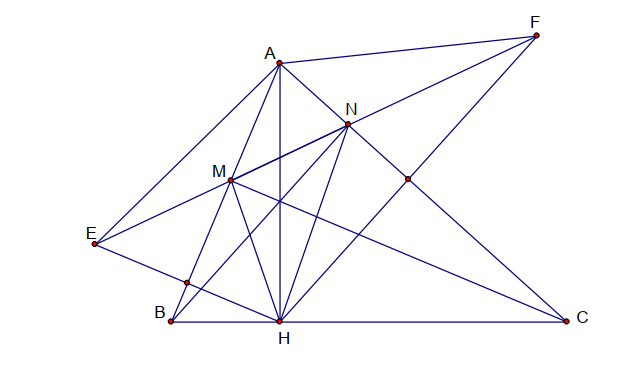
\includegraphics[width=0.7\textwidth]{1-4-lg.png}
    \begin{enumerate}
        \item Vì $\mathrm{AB}$ là trung trực của $\mathrm{EH}$ nên ta có: $\mathrm{AE}=\mathrm{AH}$ (1) \\[10pt]
        Vì $\mathrm{AC}$ là trung trực của $\mathrm{HF}$ nên ta có: $\mathrm{AH}=\mathrm{AF}$ (2) \\[10pt]
        Từ (1) và $(2)$ suy ra: $\mathrm{AE}=\mathrm{AF}$
        \item Vì $\mathrm{M} \in \mathrm{AB}$ nên $\mathrm{MB}$ là phân giác $E M H \Rightarrow \mathrm{MB}$ là phân giác ngoài góc $\mathrm{M}$ của tam giác $\mathrm{MNH}$ \\[10pt]
        Vì $\mathrm{~N} \in \mathrm{AC}$ nên $\mathrm{NC}$ là phân giác $F N H \Rightarrow \mathrm{NC}$ là phân giác ngoài góc $\mathrm{N}$ của tam giác MNH \\[10pt]
        Do $\mathrm{MB}$; $\mathrm{NC}$ cắt nhau tại $\mathrm{A}$ nên $\mathrm{HA}$ là phân giác trong góc $\mathrm{H}$ của tam giác $\mathrm{HMN}$ hay HA là phân giác của $M H N$.
        \item Ta có $\mathrm{AH} \perp \mathrm{BC}$ (gt) mà $\mathrm{HM}$ là phân giác $M H N \Rightarrow \mathrm{HB}$ là phân giác ngoài góc $\mathrm{H}$ của tam giác $\mathrm{HMN}$ \\[10pt]
        $M B$ là phân giác ngoài góc $M$ của tam giác $\mathrm{HMN}(\mathrm{cmt}) \Rightarrow \mathrm{NB}$ là phân giác trong góc $\mathrm{N}$ của tam giác $\mathrm{HMN}$ \\[10pt]
        $\Rightarrow \mathrm{BN} \perp \mathrm{AC}$ ( Hai đường phân giác của hai góc kề bù thì vuông góc với nhau). $\Rightarrow$ $\mathrm{BN} / / \mathrm{HF}$ ( cùng vuông góc với $\mathrm{AC}$ )
        Chứng minh tương tự ta có: $\mathrm{EH} / / \mathrm{CM}$
    \end{enumerate}
}
\end{bt}
	\section{Đề số 2}

\begin{bt} 
    \begin{enumerate}[a.]
        \item Thực hiện phép tính: $\mathrm{A}=\frac{2^{12} \cdot 3^5-4^6 \cdot 9^2}{2^2 \cdot 3^6+8^4 \cdot 3^5}-\frac{5^{10} .7^3-25^5 .49^2}{125.7^3+5^9 \cdot 14^3}$
        \item Tính giá trị biểu thức: $\quad B=1.2 .3+2.3 .4+3.4 .5+4.5 .6+\ldots+17.18 .19$
        \item Tìm một số tự nhiên có 3 chữ số, biết rằng nếu tăng chữ số hàng trăm thêm $\mathrm{n}$ đơn vị đồng thời giảm chữ số hàng chục và giảm chữ số hàng đơn vị đi n đơn vị thì được một số có 3 chữ số gấp n lần số có 3 chữ số ban đầu.
    \end{enumerate}
\loigiai{} 
\end{bt}

\begin{bt}
    \begin{enumerate}[a.]
        \item Tìm các số $x, y, z$ biết rằng: $\quad 3 x=4 y, 5 y=6 z$ và $x y z=30$.
        \item Tìm $x$ biết:
    $$
    \left|\mathrm{x}-\frac{1}{2}\right|+\frac{3}{4}=\left|-1,6+\frac{3}{5}\right|
    $$
    \end{enumerate}
\loigiai{} 
\end{bt}

\begin{bt}
    \begin{enumerate}[1.]
        \item Cho hàm số $\mathrm{y}=\mathrm{f}(\mathrm{x})=(\mathrm{m}-1) \mathrm{x}$
           \begin{enumerate}[a.]
            \item Tìm m biết: $f(2)-f(-1)=7$.
            \item Cho $m=5$. Tìm $x$ biết $f(3-2 x)=20$
           \end{enumerate}
        \item Cho các đơn thức $\mathrm{A}=-\frac{1}{2} \mathrm{x}^2 \mathrm{yz}^2, \mathrm{~B}=-\frac{3}{4} \mathrm{xy}^2 \mathrm{z}^2, \mathrm{C}=\mathrm{x}^3 \mathrm{y}$\\
        Chứng minh rằng các đơn thức $\mathrm{A}, \mathrm{B}, \mathrm{C}$ không thể cùng nhận giá trị âm.
    \end{enumerate}
\loigiai{} 
\end{bt}

\begin{bt}
    Cho $\triangle \mathrm{ABC}$ nhọn có góc $\mathrm{A}$ bằng $60^{\circ}$. Phân giác $\mathrm{ABC}$ cắt $\mathrm{AC}$ tại $\mathrm{D}$, phân giác $\mathrm{ACB}$ cắt $A B$ tại E. BD cắt $C E$ tại I.
    \begin{enumerate}[a.]
    \item Tính số đo góc BIC.
    \item Trên cạnh $\mathrm{BC}$ lấy điểm $\mathrm{F}$ sao cho $\mathrm{BF}=\mathrm{BE}$. Chứng minh $\Delta \mathrm{CID}=\Delta \mathrm{CIF}$.
    \item Trên tia IF lấy điểm $\mathrm{M}$ sao cho $\mathrm{IM}=\mathrm{IB}+\mathrm{IC}$. Chứng minh $\triangle \mathrm{BCM}$ là tam giác đều.
    \end{enumerate}
\loigiai{}
\end{bt}

\begin{bt}
    Tìm số tự nhiên $\mathrm{n}$ thỏa mãn điều kiện: $\quad 2 \cdot 2^2+3 \cdot 2^3+4 \cdot 2^4+\ldots+\mathrm{n} \cdot 2^{\mathrm{n}}=2^{\mathrm{n}+11}$
\loigiai{}
\end{bt}
	\onehalfspacing
\section{Đề số 3}
\graphicspath{{./img/}}
\begin{bt} 
    Cho $\mathrm{x}, \mathrm{y}, \mathrm{z}$ là các số khác 0 và $\mathrm{x}^2=\mathrm{yz}, \mathrm{y}^2=\mathrm{xz}, \mathrm{z}^2=\mathrm{xy}$.\linebreak[2]
    Chứng minh rằng: $\mathrm{x}=\mathrm{y}=\mathrm{z}$.
\loigiai{
    Vì $\mathrm{x}, \mathrm{y}$, $\mathrm{z}$ là các số khác 0 và $\mathrm{x}^2=\mathrm{yz}, \mathrm{y}^2=\mathrm{xz}, \mathrm{z}^2=\mathrm{xy}$ \\[5px]
     $\Rightarrow \frac{x}{y}=\frac{z}{x} ; \frac{y}{z}=\frac{x}{y} ; \frac{z}{x}=\frac{y}{z}$\\[5px] 
     $\Rightarrow \frac{x}{y}=\frac{y}{z}=\frac{z}{x}$\\[5px] 
     Áp dụng tính chất dãy tỉ số bằng nhau $\Rightarrow \frac{x}{y}=\frac{y}{z}=\frac{z}{x}=\frac{x+y+z}{y+z+x}=1 \Rightarrow x=y=z$
} 
\end{bt}

\begin{bt}
    \hfill
    \begin{enumerate}[a.]
        \item Tìm $x$ biết: $5^x+5^{x+2}=650$
        \item Tìm số hữu tỷ $x, y$ biết: $(3 x-33)^{2008}+|y-7|^{2009} \leq 0$
    $$
    \left|\mathrm{x}-\frac{1}{2}\right|+\frac{3}{4}=\left|-1,6+\frac{3}{5}\right|
    $$
    \end{enumerate}
\loigiai{
    \begin{enumerate}
        \item $
            5^x+5^{x+2}=650 \\[5px]
            \Leftrightarrow 5^x\left(1+5^2\right)=650 \\[5px]
            \Leftrightarrow 5^x .26=650 \\[5px]
            \Leftrightarrow \quad 5^x=25 \\[5px]
            \Leftrightarrow \quad 5^x=5^2 \\[5px]
            \Rightarrow x=2
            $
        \item $
            \text {Ta có }(3 \mathrm{x}-33)^{2008} \geq 0 \\[5px]
            |y-7|^{2009} \geq 0 \\[5px]
            \text { Suy ra }(3 \mathrm{x}-33)^{2008}+|y-7|^{2009} \geq 0 \\[5px]
            \text { Mà } \quad(3 \mathrm{x}-33)^{2008}+|y-7|^{2009} \leq 0 \text { (Theo đề bài ) } \\[5px]
            \text { Nên }(3 \mathrm{x}-33)^{2008}+|y-7|^{2009}=0 \\[5px]
            \Leftrightarrow(3 \mathrm{x}-33)^{2008}=0 \text { và }|y-7|^{2009}=0 \\[5px]
            \Leftrightarrow \mathrm{x}=11 \text { và } \mathrm{y}=7
            $
    \end{enumerate}
} 
\end{bt}

\begin{bt}
    Cho hàm số : $\mathrm{f}(\mathrm{x})=\mathrm{a} .\mathrm{x}^2+\mathrm{b} . \mathrm{x}+\mathrm{c}$ với $\mathrm{a}, \mathrm{b}, \mathrm{c}, \mathrm{d} \in \mathrm{Z}$

    Biết $f(1) \vdots 3 ; f(0) \vdots 3 ; f(-1) \vdots 3$. Chứng minh rằng $\mathrm{a}, \mathrm{b}, \mathrm{c}$ đều chia hết cho 3
\loigiai{
    Ta có: $\mathrm{f}(0)=\mathrm{c} ; \mathrm{f}(1)=\mathrm{a}+\mathrm{b}+\mathrm{c} ; \mathrm{f}(-1)=\mathrm{a}-\mathrm{b}+\mathrm{c}$
$$
\begin{aligned}
& \text { +) } f(0) \vdots 3 \Rightarrow c \vdots 3 \\[5px]
& \text { +) } f(1) \vdots 3 \Rightarrow a+b+c \vdots 3 \Rightarrow a+b \vdots 3(1) \\[5px]
& \text { +) } f(-1) \vdots 3 \Rightarrow a-b+c \vdots 3 \Rightarrow a-b \vdots 3(2)
\end{aligned}
$$
Từ (1) và (2) Suy ra $(\mathrm{a}+\mathrm{b})+(\mathrm{a}-\mathrm{b}) \vdots 3 \Rightarrow 2 a \vdots 3 \Rightarrow a \vdots 3$ vì $(2 ; 3)=1 \Rightarrow b \vdots 3$\\[5px]
Vậy a , b , c đều chia hết cho 3
} 
\end{bt}

\begin{bt}
    Cho tam giác $\mathrm{ABC}, \mathrm{AD}$ là tia phân giác của góc $\mathrm{A}$ và $B>C$.
    \begin{enumerate}[a.]
    \item Chứng minh rằng $A D C-A D B=B-C$.
    \item Vẽ đường thẳng $\mathrm{AH}$ vuông góc $\mathrm{BC}$ tại $\mathrm{H}$. Tính $A D B$ và $H A D$ khi biết $B-C=40^{\circ}$
    \item Vẽ đường thẳng chứa tia phân giác ngoài của góc đỉnh $\mathrm{A}$, nó cắt đường thẳng $\mathrm{BC}$
    tại E. 
    
    Chứng minh rằng $A E B=H A D=\frac{B-C}{2}$
    \end{enumerate}
\loigiai{
    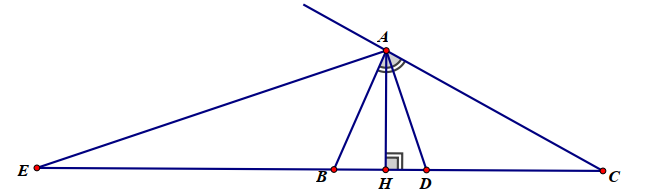
\includegraphics[width=0.7\textwidth]{3-4-lg.png}
    \begin{enumerate}
        \item $A D C=B+B A D \quad($ góc ngoài $\triangle \mathrm{ABD})(1)$\\[5px]
        $A D B=C+C A D$ ( góc ngoài $\triangle \mathrm{ADC})(2)$
        Mà $\mathrm{AD}$ là phân giác góc $\mathrm{BAD}$ nên $B A D=D A C(3)$\\[5px]
        Từ $(1),(2)$ và (3) suy ra đpcm
        \item
        Ta có:
        $$
        \begin{aligned}
        & A D C-A D B=B-C=40^{\circ} \\[5px]
        & A D C+A D B=180^{\circ} \\[5px]
        & \Rightarrow A D C=\frac{180^{\circ}+40^{\circ}}{2}=110^{\circ} ; A D B=70^{\circ} \\[5px]
        & \Rightarrow A H D=20^{\circ}
        \end{aligned}
        $$
        \item
        Ta có $\mathrm{AD}, \mathrm{AE}$ là hai tia phân giác của hai góc kê bù đỉnh $\mathrm{A}$ nên $\mathrm{AD} \perp \mathrm{AE}$\\[5px]
        Xét $\triangle \mathrm{AED} \quad$ ta có: $A E B+A D E=90^{\circ}$ (4)\\[5px]
        Xét $\triangle \mathrm{AHD}$ ta có: $H A D+A D E=90^{\circ}$ (5)\\[5px]
        Mặt khác\\[5px]
        $A D B=C+D A C=C+\frac{A}{2}$ \\[5px]
        $A+B+C=180^{\circ}$ \\[5px]
        $\Rightarrow \frac{A}{2}=90^{\circ}-\frac{B+C}{2}$ \\[5px]
        $A D B=C+90^{\circ}-\frac{B+C}{2}$ \\[5px]
        $\quad=\frac{C-B}{2}+90^{\circ}$ \\[5px]
        $\frac{\mathrm{B}-C}{2}+A D B=90^{\circ}(6)$\\[5px]
        Từ (4), (5) và (6) suy ra đpcm
    \end{enumerate}
}
\end{bt}

\begin{bt}
    \hfill
    \begin{enumerate}[a.]
        \item  Cho $S=1-\frac{1}{2}+\frac{1}{3}-\frac{1}{4}+\ldots+\frac{1}{2011}-\frac{1}{2012}+\frac{1}{2013}$ và $P=\frac{1}{1007}+\frac{1}{1008}+\ldots+\frac{1}{2012}+\frac{1}{2013}$.
        
        Tính $(S-P)^{2013}$.
        \item Cho $\mathrm{A}=\frac{\sqrt{x}+1}{\sqrt{x}-3}$
        
        Tìm $\mathrm{x} \in \mathrm{Z}$ để $\mathrm{A}$ có giá trị là một số nguyên.
    \end{enumerate}
\loigiai{
    \begin{enumerate}
        \item Ta có: \\[5px]
        $$
\begin{aligned}
& P=\frac{1}{1007}+\frac{1}{1008}+\ldots+\frac{1}{2012}+\frac{1}{2013} \\[5px]
& =\left(1+\frac{1}{2}+\frac{1}{3}+\ldots+\frac{1}{1006}+\frac{1}{1007}+\frac{1}{1008}+\ldots+\frac{1}{2012}+\frac{1}{2013}\right)-\left(1+\frac{1}{2}+\frac{1}{3}+\ldots+\frac{1}{1006}\right) \\[5px]
& =\left(1+\frac{1}{2}+\frac{1}{3}+\ldots+\frac{1}{1006}+\frac{1}{1007}+\frac{1}{1008}+\ldots+\frac{1}{2012}+\frac{1}{2013}\right)-2\left(\frac{1}{2}+\frac{1}{4}+\frac{1}{6}+\ldots+\frac{1}{2012}\right) \\[5px]
& =1-\frac{1}{2}+\frac{1}{3}-\frac{1}{4}+\ldots \ldots-\frac{1}{2012}+\frac{1}{2013}=S .
\end{aligned}
$$
Do đó $(S-P)^{2013}=0$
\item
Tìm $x \in z$ đề $A \in Z$
$$
\mathrm{A}=\frac{\sqrt{x}+1}{\sqrt{x}-3}=1+\frac{4}{\sqrt{x}-3} \quad(\mathrm{dk} \quad \mathrm{x} \geq 0, \mathrm{x} \neq 9)
$$
A nguyên khi $\frac{4}{\sqrt{x}-3}$ nguyên $\Rightarrow \sqrt{x}-3$ là Ư (4)
$$
\text{Ư}(4)=\{-4 ;-2 ;-1 ; 1 ; 2 ; 4\}
$$
Các giá trị của $x$ là : $1 ; 4 ; 16 ; 25 ; 49$.
    \end{enumerate}
}
\end{bt}
	\section{Đề số 4}

\begin{bt} 
   \hfill
   \begin{enumerate}[a.]
    \item Thực hiện phép tính: $\mathrm{A}=\left[\left(\frac{2}{193}-\frac{3}{386}\right) \cdot \frac{193}{17}+\frac{33}{34}\right]:\left[\left(\frac{7}{1931}+\frac{11}{3862}\right) \cdot \frac{1931}{25}+\frac{9}{2}\right]$.
    \item Rút gọn :    
    $$
    \mathrm{B}=(-5)^0+(-5)^1+(-5)^2+(-5)^3+\ldots+(-5)^{2016}+(-5)^{2017}
    $$
   \end{enumerate}
\loigiai{} 
\end{bt}

\begin{bt}
    \hfill
    \begin{enumerate}[a.]
        \item Tìm a, b, c biết $\quad \frac{12 a-15 b}{7}=\frac{20 c-12 a}{9}=\frac{15 b-20 c}{11}$ và $a+b+c=48$.
        \item Một công trường dự định phân chia số đất cho ba đội I, II, III tỉ lệ với 7; 6; 5 . Nhưng sau đó vì số người của các đội thay đổi nên đã chia lại tỉ lệ với $6 ; 5 ; 4$. Như vậy có một đội làm nhiều hơn so với dự định là $6 \mathrm{m}^3$ đất. Tính tổng số đất đã phân chia cho các đội.
    \end{enumerate}
\loigiai{} 
\end{bt}

\begin{bt}
   \hfill
   \begin{enumerate}[a.]
    \item Tìm giá trị nhỏ nhất của biểu thức: $C=\frac{|x-2017|+2018}{|x-2017|+2019}$.
    \item Chứng tỏ rằng $\mathrm{S}=\frac{3}{4}+\frac{8}{9}+\frac{15}{16}+\ldots+\frac{\mathrm{n}^2-1}{\mathrm{n}^2}$ không là số tự nhiên với mọi $\mathrm{n} \in \mathrm{N}, \mathrm{n}>$2.
    \item Tìm tất cả các cặp số nguyên $x$, $y$ sao cho: $x-2 x y+y=0$.
   \end{enumerate}
\loigiai{} 
\end{bt}

\begin{bt}
    Cho tam giác cân $A B C, A B=A C$. Trên cạnh $B C$ lấy điểm $D$, trên tia đối của $C B$ lấy điểm $\mathrm{E}$ sao cho $\mathrm{BD}=\mathrm{CE}$. Các đường thẳng vuông góc với $\mathrm{BC}$ kẻ từ $\mathrm{D}$ và $\mathrm{E}$ cắt $\mathrm{AB}$ và $A C$ lân lượt ở $M$ và $N$. Chứng minh rằng: 
    \begin{enumerate}[a.]
    \item $\mathrm{DM}=\mathrm{EN}$.
    \item Đường thẳng $\mathrm{BC}$ cắt $\mathrm{MN}$ tại điểm $\mathrm{I}$ là trung điểm của $\mathrm{MN}$.
    \item Đường thẳng vuông góc với $\mathrm{MN}$ tại I luôn luôn đi qua một điểm cố định khi $\mathrm{D}$ thay đổi trên cạnh BC.
    \end{enumerate}
\loigiai{}
\end{bt}

\begin{bt}
    \hfill
    Trong hình bên, đường thẳng $\mathrm{OA}$ là đồ thị của hàm số $\mathrm{y}=\mathrm{f}(\mathrm{x})=\mathrm{ax}$.
    \begin{enumerate}[a.]
        \item  Tính tỉ số $\frac{\mathrm{y}_0-2}{\mathrm{x}_0-4}$.
        \item Giả sử $x_0=5$. Tính diện tích tam giác $\mathrm{OBC}$
    \end{enumerate}
\loigiai{}
\end{bt}
	\onehalfspacing
\section{Đề số 5}

\begin{bt} 
	\hfill
	\begin{enumerate}[a.]
		\item Tìm $x, y$ biết: $\frac{4+\mathrm{x}}{7+\mathrm{y}}=\frac{4}{7}$ và $\mathrm{x}+\mathrm{y}=22$
		\item Cho $\frac{x}{3}=\frac{y}{4}$ và $\frac{y}{5}=\frac{z}{6}$. Tính $M=\frac{2 x+3 y+4 z}{3 x+4 y+5 z}$
	\end{enumerate}
	\loigiai{} 
\end{bt}

\begin{bt}
	Thực hiện tính:
	\begin{enumerate}[a.]
		\item $S=2^{2010}-2^{2009}-2^{2008} \ldots-2-1$
		\item $\mathrm{P}=1+\frac{1}{2}(1+2)+\frac{1}{3}(1+2+3)+\frac{1}{4}(1+2+3+4)+\ldots+\frac{1}{16}(1+2+3+\ldots+16)$
	\end{enumerate}
	\loigiai{} 
\end{bt}

\begin{bt}
	Tìm x biết:
	\begin{enumerate}[a.]
		\item 
		 $\frac{1}{4} \cdot \frac{2}{6} \cdot \frac{3}{8} \cdot \frac{4}{10} \cdot \frac{5}{12} \ldots \frac{30}{62} \cdot \frac{31}{64}=2^{\mathrm{x}}$
		\item $\frac{4^5+4^5+4^5+4^5}{3^5+3^5+3^5} \cdot \frac{6^5+6^5+6^5+6^5+6^5+6^5}{2^5+2^5}=2^x$
	\end{enumerate}
	\loigiai{} 
\end{bt}

\begin{bt}
	Cho tam giác $A B C$ có $B<90^{\circ}$ và $B=2 C$. Kẻ đường cao $A H$. Trên tia đối của tia $B A$ lấy điểm $\mathrm{E}$ sao cho $\mathrm{BE}=\mathrm{BH}$. Đường thẳng $\mathrm{HE}$ cắt $\mathrm{AC}$ tại $\mathrm{D}$. 
	\begin{enumerate}[a.]
		\item Chứng minh $\mathrm{BEH}=\mathrm{ACB}$
		\item Chứng $\operatorname{minh} \mathrm{DH}=\mathrm{DC}=\mathrm{DA}$.
		\item Lấy $\mathrm{B}^{\prime}$ sao cho $\mathrm{H}$ là trung điểm của $\mathrm{BB}^{\prime}$. Chứng minh tam giác $\mathrm{AB}^{\prime} \mathrm{C}$ cân.
		\item Chứng minh $\mathrm{AE}=\mathrm{HC}$.
	\end{enumerate}
	\loigiai{}
\end{bt}
	\onehalfspacing
\section{Đề số 6}
\graphicspath{{./img/}}
\begin{bt} 
	Tính hợp lý các biểu thức sau:
	\begin{enumerate}[a.]
		\item $27 \frac{1}{4} \cdot \frac{5}{8}-13 \frac{1}{4} \cdot \frac{5}{8}$
		\item $2\left|\frac{1}{2}-\frac{3}{4}\right|+\sqrt{\frac{4}{9}}$
		\item $\frac{2^2 \cdot 10+2^3 \cdot 6}{2^2 \cdot 15-2^4}$
	\end{enumerate}
	\loigiai{
		\begin{enumerate}
			\item $27 \frac{1}{4} \cdot \frac{5}{8}-13 \frac{1}{4} \cdot \frac{5}{8}=\frac{5}{8}\left(27 \frac{1}{4}-13 \frac{1}{4}\right)=14 \cdot \frac{5}{8}=\frac{35}{4}$
			\item $2\left|\frac{1}{2}-\frac{3}{4}\right|+\sqrt{\frac{4}{9}}=2\left|\frac{1}{4}\right|+\frac{2}{3}=\frac{1}{2}+\frac{2}{3}=\frac{7}{6}$
			\item $\frac{2^2 \cdot 10+2^3 \cdot 6}{2^2 \cdot 15-2^4}=\frac{2^3 \cdot 5+2^3 \cdot 6}{2^2 \cdot 15-2^4}=\frac{2^3(5+6)}{2^2\left(15-2^2\right)}=\frac{2 \cdot 11}{11}=2$ 
		\end{enumerate}
	} 
\end{bt}

\begin{bt}
	Tìm x biết:
	\begin{enumerate}[a.]
		\item $3(x-2)+\frac{2}{5}=4$
		\item $\left|x+\frac{1}{3}\right|-5=7$
		\item $(2 x-1)^7=(2 x-1)^5$
	\end{enumerate}
	\loigiai{
		\begin{enumerate}
			\item $3(x-2)+\frac{2}{5}=4\\[5px] \Leftrightarrow 3(x-2)=4-\frac{2}{5}\\[5px] \Leftrightarrow 3(x-2)=\frac{18}{5}\\[5px] \Leftrightarrow x-2=\frac{6}{5} \Leftrightarrow x=\frac{16}{5}$
			\item $\left|x+\frac{1}{3}\right|-5=7\\[5px] \Leftrightarrow\left|x+\frac{1}{3}\right|=12\\[5px] \Leftrightarrow\left[\begin{array}{c}x+\frac{1}{3}=12 \\[5px] x+\frac{1}{3}=-12\end{array} \Leftrightarrow\left[\begin{array}{c}x=\frac{35}{3} \\[5px] x=-\frac{37}{3}\end{array}\right.\right.$
			\item $(2 x-1)^7=(2 x-1)^5\\[5px] \Leftrightarrow(2 x-1)^5\left((2 x-1)^2-1\right)=0\\[5px] \Leftrightarrow\left[\begin{array}{l}2 x-1=0 \\[5px] {\left[\begin{array}{l}2 x-1=1 \\[5px] 2 x-1=-1\end{array} \Leftrightarrow\left[\begin{array}{l}x=\frac{1}{2} \\[5px] x=1 \\[5px] x=0\end{array}\right.\right.}\end{array}\right.$
		\end{enumerate}
	} 
\end{bt}

\begin{bt}
	Ba đội cùng chuyển một khối lượng gạch như nhau. Thời gian để đội thứ nhất, đội 
	thứ hai và đội thứ ba làm xong công việc lần lượt là 2 giờ, 3 giờ, 4 giờ. Tính số 
	người tham gia làm việc của mỗi đội, biết rằng số người của đội thứ ba ít hơn số 
	người của đội thứ hai là 5 người.
	\loigiai{
		Gọi số người tham gia làm việc của đội thứ nhất, đội thứ hai, đội thứ ba lân lượt là $\mathrm{x} ; \mathrm{y} ; \mathrm{z}$ (giờ).\\[5px]
ĐK: $x ; y ; z>0$\\[5px]
Cùng một khối lượng công việc, số người tham gia và thời gian làm việc tỷ lệ lệ nghịch.\\[5px]
Theo bài ra ta có: $2 \mathrm{x}=3 \mathrm{y}=4 \mathrm{z}$ và $\mathrm{y}-\mathrm{z}=5$
$$
\begin{aligned}
& \frac{y}{\frac{1}{3}}=\frac{z}{\frac{1}{4}}=\frac{y-z}{\frac{1}{3}-\frac{1}{4}}=\frac{5}{\frac{1}{12}}=60 \\[5px]
& \mathrm{y}=20, \mathrm{z}=15, \mathrm{x}=30 \text { (thoả mãn điều kiện bài toán) }
\end{aligned}
$$
Vậy số người tham gia làm việc của đội thứ nhất, đội thứ hai, đội thứ ba lân lượt là 30 người, 20 người, 15 người.
	} 
\end{bt}

\begin{bt}
	Cho tam giác $\mathrm{ABC}$ vuông tại $\mathrm{A}$ với $\frac{A B}{A C}=\frac{3}{4}$ và $\mathrm{BC}=15 \mathrm{~cm}$. Tia phân giác góc $\mathrm{C}$ cắt $A B$ tại $D$. Kẻ $D E \perp B C(E \in B C)$.
	\begin{enumerate}[a.]
		\item Chứng minh $\mathrm{AC}=\mathrm{CE}$.
		\item Tính độ dài $\mathrm{AB} ; \mathrm{AC}$.
		\item Trên tia $\mathrm{AB}$ lấy điểm $\mathrm{F}$ sao cho $\mathrm{AF}=\mathrm{AC}$. Kẻ tia $\mathrm{Fx} \perp \mathrm{FA}$ cắt tia $\mathrm{DE}$ tại $\mathrm{M}$. Tính $D C M$
	\end{enumerate}
	\loigiai{
		$$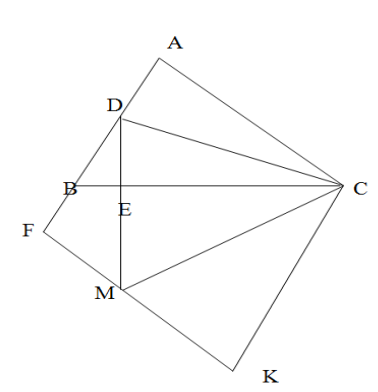
\includegraphics[width=0.45\textwidth]{6-4-lg.png}$$
		\begin{enumerate}
			\item $\mathrm{C} / \mathrm{m}$ được $\triangle A C D=\triangle E C D$ ( cạnh huyền- góc nhọn)\\[5px]
			$\Rightarrow \mathrm{AC}=\mathrm{CE}$ (hai cạnh tưong ứng)
			\item$ \frac{A B}{A C}=\frac{3}{4}(g t) \Leftrightarrow \frac{A B}{3}=\frac{A C}{4} \\[5px]
			 \Leftrightarrow \frac{A B^2}{9}=\frac{A C^2}{16}=\frac{A B^2+A C^2}{9+16}=\frac{B C^2}{25}=\frac{15^2}{25}=9 \\[5px]
			A B^2=9.9=81 \Rightarrow A B=9 \mathrm{~cm} \\[5px]
			A C^2=9.16=144 \Rightarrow A C=12 \mathrm{~cm}
			$
			\item Kẻ $\mathrm{Cy} \perp \mathrm{Fx}$ cắt nhau tại $\mathrm{K}$\\[5px]
			Ta thấy $\mathrm{AC}=\mathrm{AF}=\mathrm{FK}=\mathrm{CK}=\mathrm{CE}$ và $A C K=90^{\circ}$\\[5px]
			C/M được $\triangle C E M=\Delta C K M$ ( cạnh huyên- cạnh góc vuông)\\[5px]
			$\Rightarrow E C M=K C M$ (hai góc tương ứng)\\[5px]
			$
			D C M=D C E+E C M=\frac{1}{2} A C K=\frac{1}{2} \cdot 90^{\circ}=45^{\circ}
			$
		\end{enumerate}
	}
\end{bt}

\begin{bt}
	
	Tìm giá trị lớn nhất của biêu thức: $\mathrm{A}=|x|-|x-2|$
	\loigiai{
		Xét các trường hợp:
		\begin{enumerate}[+]
			\item TH1: $ x \geq 2 \Rightarrow A=x-(x-2)=2$ 
			\item TH2: $ 0 \leq x<2 \Rightarrow A=x+x-2=2 x-2<2$
			\item TH3: $ x<0 \Rightarrow A=-x+x-2=-2<2$
		\end{enumerate}
		$\Rightarrow$ Với mọi giá trị của $\mathrm{x}$ thì $\mathrm{A} \leq 2$\\[5px]
Vậy giá trị lớn nhất của $\mathrm{A}$ bằng 2 khi $\mathrm{x} \geq 2$
	}
\end{bt}
	\onehalfspacing
\section{Đề số 7}
\graphicspath{{./img/}}
\begin{bt} 
	\hfill
	\begin{enumerate}[1.]
		\item Tính $M=\left(\frac{0,4-\frac{2}{9}+\frac{2}{11}}{1,4-\frac{7}{9}+\frac{7}{11}}-\frac{\frac{1}{3}-0,25+\frac{1}{5}}{1 \frac{1}{6}-0,875+0,7}\right): \frac{2012}{2013}$
		\item Tìm $x$, biết: $\left|x^2+\right| x-1||=x^2+2$.
	\end{enumerate}
	\loigiai{
		\begin{enumerate}
			\item Ta có:\\
			$
			M=\left(\frac{0,4-\frac{2}{9}+\frac{2}{11}}{1,4-\frac{7}{9}+\frac{7}{11}}-\frac{\frac{1}{3}-0,25+\frac{1}{5}}{1 \frac{1}{6}-0,875+0,7}\right): \frac{2012}{2013}\\
			=\left(\frac{\frac{2}{5}-\frac{2}{9}+\frac{2}{11}}{\frac{7}{5}-\frac{7}{9}+\frac{7}{11}}-\frac{\frac{1}{3}-\frac{1}{4}+\frac{1}{5}}{\frac{7}{6}-\frac{7}{8}+\frac{7}{10}}\right): \frac{2012}{2013}\\
			=\left(\frac{2\left(\frac{1}{5}-\frac{1}{9}+\frac{1}{11}\right)}{7\left(\frac{1}{5}-\frac{1}{9}+\frac{1}{11}\right)}-\frac{\left(\frac{1}{3}-\frac{1}{4}+\frac{1}{5}\right)}{\frac{7}{2}\left(\frac{1}{3}-\frac{1}{4}+\frac{1}{5}\right)}\right): \frac{2012}{2013}\\ 
			=\left(\frac{2}{7}-\frac{2}{7}\right): \frac{2012}{2013}=0\\
 			$
			KL: .....
			\item  Vì  $x^2+|x-1|>0 \text { nên }(1)=>x^2+|x-1|=x^2+2 \text { hay }|x-1|=2$
			\begin{enumerate}[+]
				\item Nếu $x \geq 1$ thì $\left({ }^*\right)=>x-1=2 \Rightarrow x=3$
				\item Nếu $x<1$ thì $\left(^*\right)=>x-1=-2 \Rightarrow x=-1$
			\end{enumerate}
			KL: .....
		\end{enumerate}
	} 
\end{bt}

\begin{bt}
	\hfill
	\begin{enumerate}[1.]
		\item Cho $a, b, c$ là ba số thực khác 0 , thoả mãn điều kiện:
		$$
		\frac{a+b-c}{c}=\frac{b+c-a}{a}=\frac{c+a-b}{b} \text {. }
		$$
		Hãy tính giá trị của biểu thức $B=\left(1+\frac{b}{a}\right)\left(1+\frac{a}{c}\right)\left(1+\frac{c}{b}\right)$.
		\item Ba lớp 7A, 7B, 7C cùng mua một số gói tăm từ thiện, lúc đầu số gói tăm dự định chia cho ba lớp tỉ lệ với 5:6:7 nhưng sau đó chia theo tỉ lệ 4:5:6 nên có một lớp nhận nhiều hơn dự định 4 gói. Tính tổng số gói tăm mà ba lớp đã mua.
	\end{enumerate}
	\loigiai{
		\begin{enumerate}
			\item \begin{enumerate}[+]
				\item Nếu $a+b+c \neq 0$\\
				Theo tính chất dãy tỉ số bằng nhau, ta có:\\
				$
				\frac{\mathrm{a}+\mathrm{b}-\mathrm{c}}{\mathrm{c}}=\frac{\mathrm{b}+\mathrm{c}-\mathrm{a}}{\mathrm{a}}=\frac{\mathrm{c}+\mathrm{a}-\mathrm{b}}{\mathrm{b}}=\frac{\mathrm{a}+\mathrm{b}-\mathrm{c}+\mathrm{b}+\mathrm{c}-\mathrm{a}+\mathrm{c}+\mathrm{a}-\mathrm{b}}{\mathrm{a}+\mathrm{b}+\mathrm{c}}=1 \\
				\text { mà } \frac{a+b-c}{c}+1=\frac{b+c-a}{a}+1=\frac{c+a-b}{b}+1=2 \\
				\Rightarrow \frac{a+b}{c}=\frac{b+c}{a}=\frac{c+a}{b}=2 \\
				\text { Vậy B }=\left(1+\frac{b}{a}\right)\left(1+\frac{a}{c}\right)\left(1+\frac{c}{b}\right)=\left(\frac{b+a}{a}\right)\left(\frac{c+a}{c}\right)\left(\frac{b+c}{b}\right)=8$ 
				\item Nếu $\mathrm{a}+\mathrm{b}+\mathrm{c}=0 \text { thì } \mathrm{a}+\mathrm{b}=-\mathrm{c}, \mathrm{b}+\mathrm{c}=-\mathrm{a}, \mathrm{c}+\mathrm{a}=-\mathrm{b}.\\
				\text { Vậy } B=\left(1+\frac{b}{a}\right)\left(1+\frac{a}{c}\right)\left(1+\frac{c}{b}\right)=\left(\frac{b+a}{a}\right)\left(\frac{c+a}{c}\right)\left(\frac{b+c}{b}\right)=\frac{-c}{a} \cdot \frac{-b}{c} \cdot \frac{-a}{b}=-1
				$
			\end{enumerate}
			\item Gọi tổng số gói tăm 3 lớp cùng mua là $x$ ( $x$ là số tự nhiên khác 0 )\\
			Số gói tăm dự định chia chia cho 3 lớp 7A, 7B, 7C lúc đầu lần lượt là: $a, b, c$\\
			Ta có: $\frac{a}{5}=\frac{b}{6}=\frac{c}{7}=\frac{a+b+c}{18}=\frac{x}{18} \Rightarrow a=\frac{5 x}{18} ; b=\frac{6 x}{18}=\frac{x}{3} ; c=\frac{7 x}{18}$ (1)\\
			Số gói tăm sau đó chia cho 3 lớp lần lượt là a', $\mathrm{b}^{\prime}, \mathrm{c}^{\prime}$, ta có:
			$$
			\frac{a^{\prime}}{4}=\frac{b^{\prime}}{5}=\frac{c^{\prime}}{6}=\frac{a^{\prime}+b^{\prime}+c^{\prime}}{15}=\frac{x}{15} \Rightarrow a^{\prime}=\frac{4 x}{15} ; b^{\prime}=\frac{5 x}{15}=\frac{x}{3} ; c^{\prime}=\frac{6 x}{15} (2)
			$$
			So sánh (1) và (2) ta có: $\mathrm{a}>\mathrm{a}^{\prime} ; \mathrm{b}=\mathrm{b}^{\prime} ; \mathrm{c}<\mathrm{c}^{\prime}$ nên lớp 7C nhận nhiều hơn lúc đầu\\
			 Vậy: $\mathrm{c}^{\prime}-\mathrm{c}=4$ hay $\frac{6 x}{15}-\frac{7 x}{18}=4 \Rightarrow \frac{x}{90}=4 \Rightarrow x=360$\\
			Vậy số gói tăm 3 lớp đã mua là 360 gói.
		\end{enumerate}
	} 
\end{bt}

\begin{bt}
	\hfill
	\begin{enumerate}[1.]
		\item Tìm giá trị nhỏ nhất của biểu thức $\mathrm{A}=|2 x-2|+|2 x-2013|$ với $x$ là số nguyên.
		\item Tìm nghiệm nguyên dương của phương trình $x+y+z=x y z$.
	\end{enumerate}
	\loigiai{
		\begin{enumerate}
			\item Ta có: \\
			$ A=|2 x-2|+|2 x-2013|=|2 x-2|+|2013-2 x| 
			\geq|2 x-2+2013-2 x|=2011$\\ 
			Dấu "=" xảy ra khi $(2 x-2)(2013-2 x) \geq 0\\ \Leftrightarrow 1 \leq x \leq \frac{2013}{2}$\\
            Do đó giá trị nhỏ nhất của A là 2011 khi $1 \leq x \leq \frac{2013}{2}$\\
			\item Vì $x, y, z$ nguyên dương nên ta giả sử $1 \leq x \leq y \leq z$\\
			Theo bài ra $1=\frac{1}{y z}+\frac{1}{y x}+\frac{1}{z x} \leq \frac{1}{x^2}+\frac{1}{x^2}+\frac{1}{x^2}=\frac{3}{x^2} \Rightarrow x^2 \leq 3 \Leftrightarrow x=1$\\
			Thay vào đầu bài ta có $1+y+z=y z \Rightarrow \mathrm{y}-\mathrm{yz}+1+\mathrm{z}=0$
			$$
			\begin{aligned}
			& \Rightarrow \mathrm{y}(1-\mathrm{z})-(1-\mathrm{z})+2=0 \\
			& \Rightarrow (\mathrm{y}-1)(\mathrm{z}-1)=2
			\end{aligned}
			$$
			TH1: $\mathrm{y}-1=1 \Rightarrow \mathrm{y}=2$ và $\mathrm{z}-1=2 \Rightarrow \mathrm{z}=3$\\
			TH2: $y-1=2 \Rightarrow y=3$ và $z-1=1 \Rightarrow z=2$\\
			Vậy có hai cặp nghiệm nguyên thỏa mãn $(1,2,3) ;(1,3,2)$
		\end{enumerate}
	} 
\end{bt}

\begin{bt}
	Cho $x A y=60^{\circ}$ có tia phân giác $\mathrm{Az}$. Từ điểm $\mathrm{B}$ trên $\mathrm{Ax}$ kẻ $\mathrm{BH}$ vuông góc với $\mathrm{Ay}$ tại $\mathrm{H}$, kẻ $\mathrm{BK}$ vuông góc với $\mathrm{Az}$ và $\mathrm{Bt}$ song song với $\mathrm{Ay}, \mathrm{Bt}$ cắt $\mathrm{Az}$ tại $\mathrm{C}$. Từ $\mathrm{C}$ kẻ $\mathrm{CM}$ vuông góc với Ay tại $M$. Chứng minh :
	\begin{enumerate}[a.]
		\item K là trung điểm của $A C$.
		\item $\triangle \mathrm{KMC}$ là tam giác đều.
		\item Cho $B K=2 \mathrm{~cm}$. Tính các cạnh $\triangle \mathrm{AKM}$.
	\end{enumerate}
	\loigiai{
		$$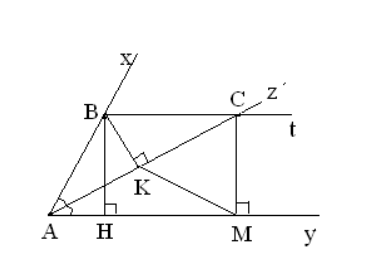
\includegraphics[width=0.45\textwidth]{7-4-lg.png}$$
		\begin{enumerate}
			\item $\triangle \mathrm{ABC}$ cân tại $\mathrm{B}$ do $C A B=A C B(=M A C)$ và $\mathrm{BK}$ là đường cao $\Rightarrow \mathrm{BK}$ là đường trung tuyến
			$\Rightarrow \mathrm{K}$ là trung điểm của $\mathrm{AC}$
			\item $\Delta \mathrm{ABH}=\Delta \mathrm{BAK}($ cạnh huyền + góc nhọn $)$\\
			$\Rightarrow \mathrm{BH}=\mathrm{AK}($ hai cạnh t.ư $)$ mà $\mathrm{AK}=\frac{1}{2} \mathrm{AC}$\\
			$\Rightarrow \mathrm{BH}=\frac{1}{2} \mathrm{AC}$\\
			Ta có : $\mathrm{BH}=\mathrm{CM}(\mathrm{t} / \mathrm{c}$ cặp đoạn chắn $)$ mà $\mathrm{CK}=\mathrm{BH}=\frac{1}{2} \mathrm{AC} \Rightarrow \mathrm{CM}=\mathrm{CK}\\ \Rightarrow \Delta \mathrm{MKC}$ là tam giác cân (1)\\
			Mặt khác: $M C B=90^{\circ}$ và $A C B=30^{\circ}$
			$
			\Rightarrow M C K=60^{\circ}(2)
			$\\ Từ (1) và (2) $\Rightarrow \Delta \Delta \mathrm{MKC}$ là tam giác đều
			\item Vì $\Delta \mathrm{ABK}$ vuông tại $\mathrm{K}$ mà góc $\mathrm{KAB}=30^{\circ} \Rightarrow \mathrm{AB}=2 \mathrm{BK}=2.2=4 \mathrm{~cm}$\\
			Vì $\triangle \mathrm{ABK}$ vuông tại $\mathrm{K}$ nên theo Pitago ta có:
			$$
			\mathrm{AK}=\sqrt{A B^2-B K^2}=\sqrt{16-4}=\sqrt{12}
			$$
			Mà $\mathrm{KC}=\frac{1}{2} \mathrm{AC} \Rightarrow \mathrm{KC}=\mathrm{AK}=\sqrt{12}$\\
			$\Delta \mathrm{KCM}$ đều $\Rightarrow \mathrm{KC}=\mathrm{KM}=\sqrt{12}$\\
			Theo phần b:\\ $\mathrm{AB}=\mathrm{BC}=4$\\
			$\mathrm{AH}=\mathrm{BK}=2$\\
			$\mathrm{HM}=\mathrm{BC}$ ( $\mathrm{HBCM}$ là hình chữ nhật $)$\\
			$\Rightarrow \mathrm{AM}=\mathrm{AH}+\mathrm{HM}=6$
			
		\end{enumerate}
	}
\end{bt}

\begin{bt}
	Cho ba số dương $0 \leq \mathrm{a} \leq \mathrm{b} \leq \mathrm{c} \leq 1$ chứng minh rằng: $\frac{a}{b c+1}+\frac{b}{a c+1}+\frac{c}{a b+1} \leq 2$
	\loigiai{
		Vì $0 \leq a \leq b \leq c \leq 1$ nên:\\
$(a-1)(b-1) \geq 0 \Leftrightarrow a b+1 \geq a+b \Leftrightarrow \frac{1}{a b+1} \leq \frac{1}{a+b} \Leftrightarrow \frac{c}{a b+1} \leq \frac{c}{a+b}$ (1)\\
Tương tự: $\frac{a}{b c+1} \leq \frac{a}{b+c}$
(2) ; $\frac{b}{a c+1} \leq \frac{b}{a+c}$ (3)\\
Do đó: $\frac{a}{b c+1}+\frac{b}{a c+1}+\frac{c}{a b+1} \leq \frac{a}{b+c}+\frac{b}{a+c}+\frac{c}{a+b}$
(4)\\
Mà $\frac{a}{b+c}+\frac{b}{a+c}+\frac{c}{a+b} \leq \frac{2 a}{a+b+c}+\frac{2 b}{a+b+c}+\frac{2 c}{a+b+c}=\frac{2(a+b+c)}{a+b+c}=2$ (5)\\
Từ (4) và (5) suy ra: $\frac{a}{b c+1}+\frac{b}{a c+1}+\frac{c}{a b+1} \leq 2 \quad$ (đpcm)
	}
\end{bt}
	\onehalfspacing
\section{Đề số 8}
\graphicspath{{./img/}}
\begin{bt} 
	\hfill
	\begin{enumerate}[a.]
		\item So sánh hai số: $(-5)^{39}$ và $(-2)^{91}$
		\item Chứng minh rằng: Số $\mathrm{A}=11^{\mathrm{n}+2}+12^{2 \mathrm{n}+1}$ chia hết cho 133 , với mọi $\mathrm{n} \in \mathrm{N}$
	\end{enumerate}
	\loigiai{
		\begin{enumerate}
			\item Ta có: $$(-5)^{39}=-5^{39}=-\left(5^3\right)^{13}=-125^{13}$$
			$$
			(-2)^{91}=-2^{91}=-\left(2^7\right)^{13}=-128^{13}
			$$
			Ta thấy: $125^{13}<128^{13} \Rightarrow-125^{13}>-128^{13} \Rightarrow(-5)^{39}>(-2)^{91}$
			\item Ta có: $\mathrm{A}=11^{\mathrm{n}+2}+12^{2 \mathrm{n}+1}=11^2 \cdot 11^{\mathrm{n}}+12 \cdot\left(12^2\right)^{\mathrm{n}}=121 \cdot 11^{\mathrm{n}}+12 \cdot 144^{\mathrm{n}}$ $=(133-12) \cdot 11^{\mathrm{n}}+12 \cdot 144^{\mathrm{n}}=133 \cdot 11^{\mathrm{n}}-12 \cdot 11^{\mathrm{n}}+12 \cdot 144^{\mathrm{n}}$\\[5px] $=133.11^{\mathrm{n}}+12 \cdot\left(144^{\mathrm{n}}-11^{\mathrm{n}}\right)$\\[5px]
			Ta thấy: $133.11^{\text {n}} \vdots 133$
			$$
\left(144^{\mathrm{n}}-11^{\mathrm{n}}\right) \vdots(144-11)=133 \Rightarrow 12 \cdot\left(144^{\mathrm{n}}-11^{\mathrm{n}}\right) \vdots 133
$$
Do đó suy ra: $133.11^{\mathrm{n}}+12 .\left(144^{\mathrm{n}}-11^{\mathrm{n}}\right)$ chia hết cho 133\\[5px]
Vậy: số $\mathrm{A}=11^{\mathrm{n}+2}+12^{2 \mathrm{n}+1}$ chia hết cho 133 , với mọi $\mathrm{n} \in \mathrm{N}$
		\end{enumerate}
	} 
\end{bt}

\begin{bt}
	\hfill
	\begin{enumerate}[a.]
		\item Tìm tất cả các cặp số $(x ; y)$ thỏa mãn: $(2 x-y+7)^{2012}+|x-3|^{2013} \leq 0$
		\item Tìm số tự nhiên $\mathrm{n}$ và chữ số $\mathrm{a}$ biết rằng: $1+2+3+\ldots+n=\overline{a a a}$
	\end{enumerate}
	\loigiai{
		\begin{enumerate}
			\item Ta có: 2012 là số tự nhiên chẵn $\Rightarrow(2 x-y+7)^{2012} \geq 0$ và $|x-3| \geq 0 \\[5px] \Rightarrow|x-3|^{2013} \geq 0$\\[5px]
			Do đó, từ $(2 x-y+7)^{2012}+|x-3|^{2013} \leq 0$\\[5px]
			suy ra: $(2 \mathrm{x}-\mathrm{y}+7)^{2012}=0$ và $|x-3|^{2013}=0$\\[5px]
			$\Rightarrow 2 \mathrm{x}-\mathrm{y}+7=0(1)$ và $\mathrm{x}-3=0(2)$\\[5px]
			Từ (2) $\Rightarrow x=3$\\[5px]
			Từ (1) $\Rightarrow \mathrm{y}=2 \mathrm{x}+7=2.3+7=13$\\[5px]
			Vậy cặp số $(x ; y)$ cần tìm là $(3 ; 13)$
			\item Ta có: $1+2+3+\ldots+n=\frac{n(n+1)}{2}$ và $\overline{a a a}=a .111=a .3 .37$\\[5px]
			Do đó, từ $1+2+3+\ldots+n=\overline{a a a} \\[5px] \Rightarrow n(n+1)=2 \cdot 3 \cdot 37 . a$ \\[5px] $\Rightarrow \mathrm{n}(\mathrm{n}+1)$ chia hết cho số nguyên tố 37\\[5px]
			$\Rightarrow \mathrm{n}$ hoặc $\mathrm{n}+1$ chia hết cho 37 (1)\\[5px]
			Mặt khác: $\frac{n(n+1)}{2}=\overline{a a a} \leq 999\\[5px] \Rightarrow \mathrm{n}(\mathrm{n}+1) \leq 1998 \Rightarrow \mathrm{n}<45$ (2)\\[5px]
			Từ (1) và (2) suy ra hoặc $n=37$, hoặc $n+1=37$\\[5px]
			- Với $\mathrm{n}=37$ thì $\overline{a a a}=\frac{37.38}{2}=703$ (không thỏa)\\[5px]
			- Với $\mathrm{n}+1=37$ thì $\overline{a a a}=\frac{36.37}{2}=666$ (thỏa mãn)\\[5px]
			Vậy $n=36$ và $a=6$.
		\end{enumerate}
	} 
\end{bt}

\begin{bt}
	Ba lớp 7 ở trường K có tất cả 147 học sinh. Nếu đưa $\frac{1}{3}$ số học sinh của lớp $7 \mathrm{~A}_1, \frac{1}{4}$ số học sinh của lớp $7 \mathrm{~A}_2$ và $\frac{1}{5}$ số học sinh của lớp $7 \mathrm{~A}_3$ đi thi học sinh giỏi cấp huyện thì số học sinh còn lại của ba lớp bằng nhau. Tính tổng số học sinh của mỗi lớp 7 ở trường K.
	\loigiai{
		Gọi tổng số học sinh của $7 \mathrm{~A}_1, 7 \mathrm{~A}_2, 7 \mathrm{~A}_3$ lần lượt là $\mathrm{a}, \mathrm{b}, \mathrm{c}\left(\mathrm{a}, \mathrm{b}, \mathrm{c} \in \mathrm{N}^*\right)$\\[5px]
        Theo bài ra ta có : $\mathrm{a}-\frac{1}{3} \mathrm{a}=\mathrm{b}-\frac{1}{4} \mathrm{~b}=\mathrm{c}-\frac{1}{5} \mathrm{c}\left({ }^*\right)$ và $\mathrm{a}+\mathrm{b}+\mathrm{c}=147$ \\[5px] Từ $\left({ }^*\right) \Rightarrow \frac{2 a}{3}=\frac{3 b}{4}=\frac{4 c}{5} \Rightarrow \frac{12 a}{18}=\frac{12 b}{16}=\frac{12 c}{15}\\[5px] \Rightarrow \frac{a}{18}=\frac{b}{16}=\frac{c}{15}$\\[5px]
        Áp dụng tính chất dãy tỷ số bằng nhau ta có :
$$
\frac{a}{18}=\frac{b}{16}=\frac{c}{15}=\frac{a+b+c}{18+16+15}=\frac{147}{49}=3 .
$$
Suy ra: $a=54, b=48, c=45$\\[5px]
Vậy tổng số học sinh của $7 \mathrm{~A}_1, 7 \mathrm{~A}_2$, $7 \mathrm{~A}_3$ lần lượt là 54,48 và 45 .
	} 
\end{bt}

\begin{bt}
	Cho tam giác $\mathrm{ABC}$ có $\hat{A}=3 \hat{B}=6 \hat{C}$.
	\begin{enumerate}[a.]
		\item Tính số đo các góc của tam giác $\mathrm{ABC}$.
		\item Kẻ $\mathrm{AD}$ vuông góc với $\mathrm{BC}$ (D thuộc $\mathrm{BC}$ ). Chứng minh: $\mathrm{AD}<\mathrm{BD}<\mathrm{CD}$.
	\end{enumerate}
	\loigiai{
		$$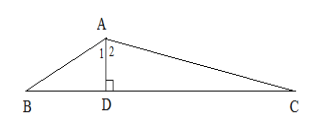
\includegraphics[width=0.55\textwidth]{8-4-lg.png}$$
		\begin{enumerate}
			\item Từ $\hat{A}=3 \hat{B}=6 \hat{C} \Rightarrow \frac{\hat{A}}{6}=\frac{\hat{B}}{2}=\frac{\hat{C}}{1}=\frac{\hat{A}+\hat{B}+\hat{C}}{6+2+1}=\frac{180^{\circ}}{9}=20^{\circ}$\\[5px] 
			$
			\begin{aligned}
				\Rightarrow \hat{A} & =6.20^{\circ}=120^{\circ} \\[5px]
				\hat{B} & =2.20^{\circ}=40^{\circ} \\[5px]
				\hat{C} & =1.20^{\circ}=20^{\circ}
				\end{aligned}
			$
			$\text { Vậy: } \hat{A}=120^{\circ} ; \hat{B}=40^{\circ} ; \hat{C}=20^{\circ}$
		    \item - Trong $\triangle \mathrm{ACD}$ có\\[5px]
			$
			\begin{aligned}
			A \hat{D} C=90^{\circ} ; \hat{C}=20^{\circ} & \Rightarrow \hat{A}_2=70^{\circ} \\[5px]
			& \Rightarrow \hat{A}_1=50^{\circ}
			\end{aligned}
			$\\[5px]
			- Xét $\triangle \mathrm{ADB}$ có $\hat{B}=40^{\circ}<\hat{A}_1=50^{\circ} \Rightarrow A D<B D$ (1)\\[5px]
			- Xét $\triangle \mathrm{ABC}$ có $\left.\hat{B}=40^{\circ}>\hat{C}=20^{\circ} \Rightarrow A B<A C \Rightarrow A B^2<A C^2{ }^*\right)$\\[5px]
			- Áp dụng định lý Pytago cho hai tam giác vuông $\mathrm{ADB}$ và $\mathrm{ADC}$ có: $\mathrm{AB}^2=\mathrm{AD}^2+\mathrm{BD}^2$ và $\mathrm{AC}^2=\mathrm{AD}^2+\mathrm{CD}^2$\\[5px]
			Do đó, từ $\left(^*\right) \Rightarrow \mathrm{AD}^2+\mathrm{BD}^2<\mathrm{AD}^2+\mathrm{CD}^2$
			$\\[5px]
			\Rightarrow \mathrm{BD}^2<\mathrm{CD}^2 \Rightarrow \mathrm{BD}<\mathrm{CD} \text { (2) }
			$\\[5px]
			Từ (1) và $(2) \Rightarrow \mathrm{AD}<\mathrm{BD}<\mathrm{CD}$
		\end{enumerate}
	}
\end{bt}

\begin{bt}
	Cho tam giác $A B C$ cân ở $A$. Trên cạnh $A B$ lấy điểm $M$, trên tia đối của tia CA lấy điểm $\mathrm{N}$ sao cho $\mathrm{AM}+\mathrm{AN}=2 \mathrm{AB}$.
	\begin{enumerate}[a.]
		\item Chứng minh rằng: $\mathrm{BM}=\mathrm{CN}$
		\item Chứng minh rằng: $\mathrm{BC}$ đi qua trung điểm của đoạn thẳng $\mathrm{MN}$.
		\item Đường trung trực của $\mathrm{MN}$ và tia phân giác của góc $\mathrm{BAC}$ cắt nhau tại $\mathrm{K}$. Chứng minh rằng: $\mathrm{KC} \perp \mathrm{AC}$.
	\end{enumerate}
	\loigiai{
		$$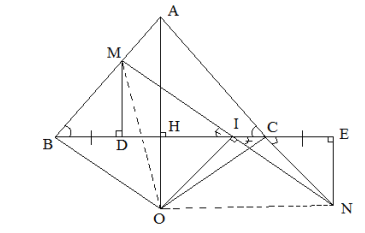
\includegraphics[width=0.55\textwidth]{4-4-lg.png}$$
		\begin{enumerate}
			\item Theo giả thiết, ta có:\\[5px]
			$
			\begin{aligned}
			& 2 \mathrm{AB}=\mathrm{AB}+\mathrm{AB}=\mathrm{AB}+\mathrm{AM}+\mathrm{BM} \\[5px]
			& \mathrm{AM}+\mathrm{AN}=\mathrm{AM}+\mathrm{AC}+\mathrm{CN} \\[5px]
			& \Delta \mathrm{ABC} \text { cân ở } \mathrm{A} \Rightarrow \mathrm{AB}=\mathrm{AC} \\[5px]
			& \text { Do đó, từ } \mathrm{AM}+\mathrm{AN}=2 \mathrm{AB} \\[5px]
			& \Rightarrow \mathrm{BM}=\mathrm{CN}
			\end{aligned}
			$
			\item Qua M kẽ $M E / / A C(E \in B C)$
			$\triangle \mathrm{ABC}$ cân ở $\mathrm{A} \Rightarrow \triangle \mathrm{BME}$ cân ở $\mathrm{M} \Rightarrow \mathrm{EM}=\mathrm{BM}=\mathrm{CN}$ $\Rightarrow \Delta \mathrm{MEI}=\Delta \mathrm{NCI}(\mathrm{g}-\mathrm{c}-\mathrm{g}) \Rightarrow \mathrm{IM}=\mathrm{IN}$\\[5px]
			Vậy: BC đi qua trung điểm của MN.
			\item $+\mathrm{K}$ thuộc đường trung trực của $\mathrm{MN} \Rightarrow \mathrm{KM}=\mathrm{KN}$ (1)\\[5px]
			$+\triangle \mathrm{ABK}=\Delta \mathrm{ACK}(\mathrm{c}-\mathrm{g}-\mathrm{c}) \Rightarrow \mathrm{KB}=\mathrm{KC} \text{ (2) } ; A \hat{B K}=A \hat{C} K\left(^*\right)$\\[5px]
			+ Kết quả câu c/m câu a $\mathrm{BM}=\mathrm{CN}$ (3)\\[5px]
			+ Từ (1), (2) và (3) $\Rightarrow \Delta \mathrm{BMK}=\Delta \mathrm{CNK}(\mathrm{c}-\mathrm{c}-\mathrm{c}) \Rightarrow A \hat{B} K=N \hat{C K} \quad\left({ }^{* *}\right)$\\[5px]
			+ Từ $\left({ }^*\right)$ và $\left({ }^{* *}\right) \Rightarrow A \hat{C} K=N \hat{C} K=\frac{180^{\circ}}{2}=90^{\circ} \Rightarrow \mathrm{KC} \perp \mathrm{AN}$
		\end{enumerate}
	}
\end{bt}
	\onehalfspacing
\section{Đề số 9}
\graphicspath{{./img/}}
\begin{bt}
	\hfill
	\begin{enumerate}[1.]
		\item Tính giá trị các biểu thức sau:
		\begin{enumerate}[a.]
			\item $\mathrm{A}=\left(\frac{-3}{7}+\frac{4}{11}\right): \frac{7}{11}+\left(\frac{-4}{7}+\frac{7}{11}\right): \frac{7}{11}$
			\item $B=\frac{2^{12} \cdot 3^5-4^6 \cdot 9^2}{\left(2^2 \cdot 3\right)^6+8^4 \cdot 3^5}$
		\end{enumerate}
		\item Cho $\frac{x}{3}=\frac{y}{5}$. Tính giá trị biểu thức: $C=\frac{5 x^2+3 y^2}{10 x^2-3 y^2}$
	\end{enumerate}
	\loigiai{
		\begin{enumerate}[1.]
			\item \begin{enumerate}
				\item $
				A=\left(\frac{-3}{7}+\frac{4}{11}\right): \frac{7}{11}+\left(\frac{-4}{7}+\frac{7}{11}\right): \frac{7}{11}=\left(\frac{-3}{7}+\frac{4}{11}\right) \cdot \frac{11}{7}+\left(\frac{-4}{7}+\frac{7}{11}\right) \cdot \frac{11}{7} \\[5px]
				A=\frac{11}{7}\left[\left(\frac{-3}{7}+\frac{4}{11}\right)+\left(\frac{-4}{7}+\frac{7}{11}\right)\right]= \frac{11}{7}\left[\left(\frac{-3}{7}+\frac{-4}{7}\right)+\left(\frac{4}{11}+\frac{7}{11}\right)\right]\\[5px]=\frac{11}{7}[(-1)+1]=\frac{11}{7} \cdot 0=0
				$
				\item $
				\mathrm{B} =\frac{2^{12} \cdot 3^5-4^6 \cdot 9^2}{\left(2^2 \cdot 3\right)^6+8^4 \cdot 3^5}=\frac{2^{12} \cdot 3^5-\left(2^2\right)^6 \cdot\left(3^2\right)^2}{2^{12} \cdot 3^6+\left(2^3\right)^4 \cdot 3^5}\\[5px]=\frac{2^{12} \cdot 3^5-2^{12} \cdot 3^4}{2^{12} \cdot 3^6+2^{12} \cdot 3^5}=\frac{2^{12} \cdot 3^4(3-1)}{2^{12} \cdot 3^5(3+1)} \\[5px]
				\mathrm{B} =\frac{2^{12} \cdot 3^4 \cdot 2}{2^{12} \cdot 3^5 \cdot 4}=\frac{1}{6}$
			\end{enumerate}
			\item  Đặt $\frac{x}{3}=\frac{y}{5}=\mathrm{k} \Leftrightarrow\left\{\begin{array}{l}x=3 \mathrm{k} \\[5px] \mathrm{y}=5 \mathrm{k}\end{array}\right.$. Khi đó:
			$$
			C=\frac{5 \mathrm{x}^2+3 \mathrm{y}^2}{10 \mathrm{x}^2-3 \mathrm{y}^2}=\frac{5(3 \mathrm{k})^2+3(5 \mathrm{k})^2}{10(3 \mathrm{k})^2-3(5 \mathrm{k})^2}=\frac{45 \mathrm{k}^2+75 \mathrm{k}^2}{90 \mathrm{k}^2-75 \mathrm{k}^2}=\frac{120 \mathrm{k}^2}{15 \mathrm{k}^2}=8
			$$
		\end{enumerate}
	} 
\end{bt}

\begin{bt}
	\hfill
	\begin{enumerate}[1.]
		\item Tìm các số $x, y, z$, biết:
		\begin{enumerate}[a.]
			\item $\frac{x}{2}=\frac{y}{3} ; \frac{y}{5}=\frac{z}{7}$ và $x+y+z=92$
			\item $(x-1)^{2018}+(2 y-1)^{2018}+|x+2 y-z|^{2019}=0$
		\end{enumerate}
		\item Tìm $x, y$ nguyên biết: $x y+3 x-y=6$
	\end{enumerate}
	\loigiai{
		\begin{enumerate}[1.]
			\item \begin{enumerate}
			\item Ta có: $\left\{\begin{array}{l}\frac{\mathrm{x}}{2}=\frac{\mathrm{y}}{3} \\[5px] \frac{\mathrm{y}}{5}=\frac{\mathrm{z}}{7}\end{array} \Leftrightarrow\left\{\begin{array}{l}\frac{\mathrm{x}}{10}=\frac{\mathrm{y}}{15} \\[5px] \frac{\mathrm{y}}{15}=\frac{\mathrm{z}}{21}\end{array} \Leftrightarrow \frac{\mathrm{x}}{10}=\frac{\mathrm{y}}{15}=\frac{\mathrm{z}}{21}\right.\right.$\\[5px]
			Áp dụng tính chất dãy tỉ số bằng nhau và $x+y+z=92$, ta được:\\[5px]
			$
		     \frac{x}{10}=\frac{y}{15}=\frac{z}{21}=\frac{x+y+z}{10+15+21}=\frac{92}{46}=2 \\[5px]
			\Rightarrow\left\{\begin{array}{l}
			\frac{x}{10}=2 \\[5px]
			\frac{y}{15}=2 \Leftrightarrow\left\{\begin{array}{l}
			x=20 \\[5px]
			y=30 \\[5px]
			z=42\\[5px]
			\end{array}\right. \\[5px]
			\frac{z}{21}=2
			\end{array}\right.
			$
			\item Ta có: \\[5px]
			$
				(\mathrm{x}-1)^{2016} \geq 0 \quad \forall \mathrm{x} \\[5px]
				(2 \mathrm{y}-1)^{2016} \geq 0 \quad \forall \mathrm{y} \\[5px]
				|\mathrm{x}+2 \mathrm{y}-\mathrm{z}|^{2017} \geq 0 \quad \forall \mathrm{x}, \mathrm{y}, \mathrm{z}\\[5px]
				 \Rightarrow(x-1)^{2016}+(2 y-1)^{2016}+|x+2 y-z|^{2017} \geq 0 \quad \forall x, y, z \\[5px]
				\text { Mà }(x-1)^{2016}+(2 y-1)^{2016}+|x+2 y-z|^{2017}=0\\[5px]
				\text { nên dấu "=" xảy ra } \Leftrightarrow\left\{\begin{array} { l } 
					{ ( \mathrm { x } - 1 ) ^ { 2 0 1 6 } = 0 } \\[5px]
					{ ( 2 \mathrm { y } - 1 ) ^ { 2 0 1 6 } = 0 } \\[5px]
					{ | \mathrm { x } + 2 \mathrm { y } - \mathrm { z } | ^ { 2 0 1 7 } = 0 }
					\end{array}\\[5px]
					 \Leftrightarrow \left\{\begin{array} { l } 
					{ \mathrm { x } = 1 } \\[5px]
					{ \mathrm { y } = \frac { 1 } { 2 } } \\[5px]
					{ 1 + 2 \cdot \frac { 1 } { 2 } - \mathrm { z } = 0 }
					\end{array}\\[5px] 
					\Leftrightarrow \left\{\begin{array}{l}
					\mathrm{x}=1 \\[5px]
					\mathrm{y}=\frac{1}{2} \\[5px]
					\mathrm{z}=2
					\end{array}\right.\right.\right.
				$
		    \end{enumerate}
			\item Ta có: $x y+3 x-y=6 \Leftrightarrow x(y+3)-(y+3)=6-3$\\[5px]
			$
			\Leftrightarrow(x-1)(y+3)=3=1.3=3.1=(-1)(-3)=(-3)(-1)
			$\\[5px]
			Ta có bảng sau:\\[5px]
			$$\begin{array}{|c|c|c|c|c|}
				\hline \mathrm{x}-1 & 1 & 3 & -1 & -3 \\[5px]
				\hline \mathrm{y}+3 & 3 & 1 & -3 & -1 \\[5px]
				\hline \mathrm{x} & 2 & 4 & 0 & -2 \\[5px]
				\hline \mathrm{y} & 0 & -2 & -6 & -4 \\[5px]
				\hline
				\end{array}$$
				\text { Vậy: }(x ; y)=(2 ; 0)=(4 ;-2)=(0 ; 6)=(-2 ;-4)
	    \end{enumerate}
	} 
\end{bt}

\begin{bt}
	\hfill
	\begin{enumerate}[1.] 
		\item Tìm đa thức $\mathrm{A}$ biết: $A-\left(3 x y-4 y^2\right)=x^2-7 x y+8 y^2$
		\item Cho hàm số $y=f(x)=a x+2$ có đồ thị đi qua điểm $A\left(a-1 ; a^2+a\right)$.
		\begin{enumerate}[a.]
			\item Tìm a
			\item Với a vừa tìm được, tìm giá trị của $x$ thỏa mãn: $f(2 x-1)=f(1-2 x)$
		\end{enumerate}
	\end{enumerate}
	\loigiai{
		\begin{enumerate}[1.]
			\item Ta có: $A-\left(3 x y-4 y^2\right)=x^2-7 x y+8 y^2$\\[5px]
			$
			\begin{aligned}
			& A=x^2-7 x y+8 y^2+\left(3 x y-4 y^2\right) \\[5px]
			& A=x^2-4 x y+4 y^2
			\end{aligned}
			$
			\item \begin{enumerate}
				\item Vì đồ thị hàm số $\mathrm{y}=\mathrm{f}(\mathrm{x})=\mathrm{ax}+2$ đi qua điểm $\mathrm{A}\left(\mathrm{a}-1 ; \mathrm{a}^2+\mathrm{a}\right)$ nên: $a^2+a=a(a-1)+2 \Leftrightarrow a^2+a=a^2-a+2 \Leftrightarrow 2 a=2 \Leftrightarrow a=1$
				\item Với $a=1$ thì $y=f(x)=x+2$\\[5px]
				Ta có: $\mathrm{f}(2 \mathrm{x}-1)=\mathrm{f}(1-2 \mathrm{x}) \Leftrightarrow(2 \mathrm{x}-1)+2=(1-2 \mathrm{x})+2 \Leftrightarrow 4 \mathrm{x}=2 \Leftrightarrow \mathrm{x}=\frac{1}{2}$
			\end{enumerate}
		\end{enumerate}
	} 
\end{bt}

\begin{bt}
	Cho tam giác $A B C$ vuông tại $A$. Vẽ về phía ngoài tam giác $A B C$ các tam giác đều $A B D$ và $A C E$. Gọi $\mathrm{I}$ là giao điểm $B E$ và $C D$. Chứng minh rằng:
	\begin{enumerate}[a.]
		\item $B E=C D$
		\item $\triangle \mathrm{BDE}$ là tam giác cân
		\item $\mathrm{EIC}=60^{\circ}$ và IA là tia phân giác của DIE
	\end{enumerate}
	\loigiai{
		GT: $\triangle \mathrm{ABC}, \mathrm{A}=90^{\circ}, \Delta \mathrm{ABD}$ và $\triangle \mathrm{ACE}$ đều,
		$\mathrm{I}=\mathrm{BE} \cap \mathrm{CD}$\\[5px] 
		KL:\\[5px] 
		\begin{enumerate}
			\item  $\mathrm{BE}=\mathrm{CD}$
			\item $\triangle \mathrm{BDE}$ là tam giác cân
			\item $\mathrm{EIC}=60^{\circ}$ và $\mathrm{IA}$ là tia phân giác của DIE
		\end{enumerate}
		$$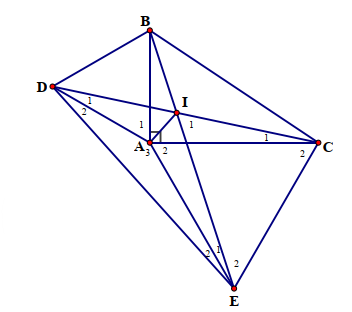
\includegraphics[width=0.55\textwidth]{9-4-lg.png}$$
		\begin{enumerate}
			\item $\text { Ta có: }\left\{\begin{array}{l}
				\mathrm{DAC}=\mathrm{A}_1+90^{\circ}=60^{\circ}+90^{\circ}=150^{\circ} \\[5px]
				\mathrm{BAE}=\mathrm{A}_2+90^{\circ}=60^{\circ}+90^{\circ}=150^{\circ}
				\end{array}\\[5px] \Rightarrow \mathrm{DAC}=\mathrm{BAE}\right.$\\[5px]
				Xét $\triangle \mathrm{DAC}$ và $\triangle \mathrm{BAE}$ có:\\[5px]
                $
                \mathrm{DA} =\mathrm{BA}(\mathrm{GT}) \\[5px]
                \mathrm{DAC} =\mathrm{BAE}(\mathrm{CM} \text { trên) } \\[5px]
                \mathrm{AC} =\mathrm{AE}(\mathrm{GT}) \\[5px]
                \Rightarrow \Delta \mathrm{DAC} =\Delta \mathrm{BAE}(\mathrm{c}-\mathrm{g}-\mathrm{c}) \Rightarrow \mathrm{BE}=\mathrm{CD} \text { (Hai cạnh tương ứng) }
                $
				\item Ta có:  $\mathrm{A}_3+\mathrm{A}_1+\mathrm{BAC}+\mathrm{A}_2=360^{\circ}$\\[5px]
				$ \Leftrightarrow A_3+60^{\circ}+90^{\circ}+60^{\circ}=360^{\circ} \\[5px]
				 \Leftrightarrow A_3=150^{\circ} \\[5px]
				 \Rightarrow A_3=D A C=150^{\circ}$\\[5px]
				 Xét $\triangle \mathrm{DAE}$ và $\triangle \mathrm{BAE}$ có:\\[5px]
				 $
				 \mathrm{DA}=\mathrm{BA}(\mathrm{GT}) \\[5px]
				 \mathrm{A}_3=\mathrm{DAC}(\mathrm{CM} \text { trên })$\\[5px]
				 AE: Cạnh chung\\[5px]
				 $\Rightarrow \triangle \mathrm{DAE}=\triangle \mathrm{BAE}(\mathrm{c}-\mathrm{g}-\mathrm{c}) \\[5px]\Rightarrow \mathrm{DE}=\mathrm{BE}$ (Hai cạnh tương ứng)\\[5px]
				 $\Rightarrow \triangle B D E$ là tam giác cân tại $E$
				 \item Ta có: $\Delta \mathrm{DAC}=\Delta \mathrm{BAE}(\mathrm{CM}$ câu $\mathrm{a}) \Rightarrow \mathrm{E}_1=\mathrm{C}_1$ (Hai góc tương ứng)
				 Lại có: $\hat{\mathrm{I}}_1+\mathrm{E}_2+\mathrm{ICE}=180^{\circ}$ (Tổng 3 góc trong $\triangle \mathrm{ICE}$ )\\[5px]
				 $
				 \Leftrightarrow \hat{\mathrm{I}}_1+\left(\mathrm{AEC}-\mathrm{E}_1\right)+\left(\mathrm{C}_1+\mathrm{C}_2\right)=180^{\circ} \\[5px]
				 \Leftrightarrow \hat{\mathrm{I}}_1+60^{\circ}-\mathrm{E}_1+\mathrm{C}_1+60^{\circ}=180^{\circ} \\[5px]
				 \Leftrightarrow \hat{\mathrm{I}}_1+120^{\circ}=180^{\circ}\left(\text{Vì } \mathrm{E}_1=\mathrm{C}_1\right)$\\[5px] 
				 $\Leftrightarrow \hat{\mathrm{I}}_1=60^{\circ}$\\[5px]
				 Vì $\triangle \mathrm{DAE}=\triangle \mathrm{BAE}\left(\mathrm{Cm}\right.$ câu b) $\Rightarrow \mathrm{E}_1=\mathrm{E}_2$ (Hai góc tương ứng)\\[5px] $\Rightarrow \mathrm{EA}$ là tia phân giác của DEI (1)\\[5px]
				 $
				 \text{Vì }\left\{\begin{array}{l}
				 \triangle \mathrm{DAC}=\Delta \mathrm{BAE} \\[5px]
				 \triangle \mathrm{DAE}=\Delta \mathrm{BAE}
				 \end{array} \Rightarrow \triangle \mathrm{DAC}=\triangle \mathrm{DAE} \Rightarrow \mathrm{D}_1=\mathrm{D}_2 \text { (Hai góc tương ứng) }\\[5px] \Rightarrow \mathrm{DA}\right. \text { là }
				 $
				 tia phân giác của EDC (2)\\[5px]
				 Từ (1) và (2) $\Rightarrow \mathrm{A}$ là giao điểm của 2 tia phân giác trong $\triangle \mathrm{DIE}\\[5px] \Rightarrow \mathrm{IA}$ là đường phân giác thứ ba trong $\triangle$ DIE hay IA là tia phân giác của DIE
		\end{enumerate}
	}
\end{bt}

\begin{bt}
	\hfill
	\begin{enumerate}[1.] 
		\item Tìm số hữu tỉ $x$, sao cho tổng của số đó với nghịch đảo của nó có giá trị là một số nguyên.
		\item Cho các số a,b,c không âm thỏa mãn: $a+3 c=2016 ; a+2 b=2017$. Tìm giá trị lớn nhất của biểu thức $P=a+b+c$.
	\end{enumerate}
	\loigiai{
		\begin{enumerate}
			\item Gọi $x=\frac{m}{n}(m, n \in Z, n \neq 0,(m, n)=1)$. Khi đó:\\[5px]
			$
			\mathrm{x}+\frac{1}{\mathrm{x}}=\frac{\mathrm{m}}{\mathrm{n}}+\frac{\mathrm{n}}{\mathrm{m}}=\frac{\mathrm{m}^2+\mathrm{n}^2}{\mathrm{mn}}(1)
			$\\[5px]
			Để $x+\frac{1}{x}$ nguyên thì $\mathrm{m}^2+n^2: \mathrm{mn}$\\[5px]
			$
			\begin{gathered}
			\Rightarrow \mathrm{m}^2+\mathrm{n}^2 \vdots \mathrm{m} \\[5px]
			\Rightarrow \quad \mathrm{n}^2: \mathrm{m}\left(\text{vì } \mathrm{m^2} \vdots \mathrm{m}\right) \\[5px]
			\Rightarrow \quad \mathrm{n} \vdots \mathrm{m} \\[5px]
			\text { Mà }(\mathrm{m}, \mathrm{n})=1 \text { nên } \mathrm{m}=1 \text { hoặc } \mathrm{m}=-1
			\end{gathered}
			$
			\begin{enumerate}[*]
				\item Với m = 1:\\[5px] 
				Từ (1), ta có: $\mathrm{x}+\frac{1}{\mathrm{x}}=\frac{1^2+\mathrm{n}^2}{1 \cdot \mathrm{n}}=\frac{1+\mathrm{n}^2}{\mathrm{n}}$. Để $\mathrm{x}+\frac{1}{\mathrm{x}}$ nguyên thì $1+\mathrm{n}^2 \vdots \mathrm{n} \Rightarrow 1 \vdots \mathrm{n}$ hay $\mathrm{n}= \pm$1
				\item Với m = -1:\\[5px]
				Từ (1), ta có: $\mathrm{x}+\frac{1}{\mathrm{x}}=\frac{(-1)^2+\mathrm{n}^2}{(-1) \cdot \mathrm{n}}=\frac{1+\mathrm{n}^2}{-\mathrm{n}}$. Để $\mathrm{x}+\frac{1}{\mathrm{x}}$ nguyên thì $1+\mathrm{n}^2:(-\mathrm{n}) \Rightarrow 1 \vdots(-\mathrm{n})$ hay $n= \pm 1$\\[5px]
                Khi đó $x=\frac{\mathrm{m}}{\mathrm{n}}=\frac{1}{1}=\frac{1}{-1}=\frac{-1}{1}=\frac{-1}{-1}$ hay $\mathrm{x}= \pm 1$
			\end{enumerate}
			\item Ta có: $\mathrm{a}+3 \mathrm{c}=2016$ (1) và $\mathrm{a}+2 \mathrm{~b}=2017$ (2)\\[5px]
			Từ (1) $\Rightarrow \mathrm{a}=2016-3 \mathrm{c}$\\[5px]
			Lấy (2) - (1) ta được: $2 \mathrm{~b}-3 \mathrm{c}=1 \Leftrightarrow \mathrm{b}=\frac{1+3 \mathrm{c}}{2}$.\\[5px]
			Khi đó:\\[5px]
			$
P=a+b+c=(2016-3 c)+\frac{1+3 c}{2}+c=\left(2016+\frac{1}{2}\right)+\frac{-6 c+3 c+2 c}{2}=2016 \frac{1}{2}-\frac{c}{2} .
$\\[5px]
Vì a, b, c không âm nên $P=2016 \frac{1}{2}-\frac{c}{2} \leq 2016 \frac{1}{2}, MaxP=2016 = \frac{1}{2}\\[5px] \Leftrightarrow \mathrm{c}=0$
		\end{enumerate}
	}
\end{bt}
	\onehalfspacing
\section{Đề số 10}
\graphicspath{{./img/}}
\begin{bt} 
	Tính giá trị của biểu thức
	\begin{enumerate}[a.]
		\item $A=\frac{4^5 \cdot 9^4-2 \cdot 6^9}{2^{10} \cdot 3^8+6^8 \cdot 20}$
		\item $\mathrm{B}=1+3+3^2+3^3+\ldots+3^{2015}-\frac{3^{2016}}{2}$
	\end{enumerate}
	\loigiai{
		\begin{enumerate}
			\item A=$\frac{2^{10} \cdot 3^8-2^{10} \cdot 3^9}{2^{10} \cdot 3^8+2^{10} \cdot 3^8 \cdot 5}=\frac{2^{10} \cdot 3^8(1-3)}{2^{10} \cdot 3^8(1+5)}=-\frac{1}{3}$
			\item Đặt $M=1+3+3^2+\ldots+3^{2015}$\\
			Ta có $3 \mathrm{M}=3+3^2+3^3+\ldots+3^{2016}$\\ $3 \mathrm{M}-\mathrm{M}=3^{2016}-1 \Rightarrow \mathrm{M}=\frac{3^{2016}}{2}-\frac{1}{2}$\\
			Khi đó $\mathrm{B}=\frac{3^{2016}}{2}-\frac{1}{2}-\frac{3^{2016}}{2}=-\frac{1}{2}$\\
		\end{enumerate}
	} 
\end{bt}

\begin{bt}
	\hfill
	\begin{enumerate}[a.]
		\item Tìm $x$ biết: $\frac{15}{28}-\left|x-\frac{3}{14}\right|=-\frac{5}{12}$
		\item Tìm $x$, y nguyên biết: $25-y^2=4(x-2016)^2$
	\end{enumerate}
	\loigiai{
		\begin{enumerate}
			\item $\left|x-\frac{3}{14}\right|=\frac{15}{28}+\frac{5}{12} \Leftrightarrow\left|x-\frac{3}{14}\right|=\frac{80}{84}$\\
			$
			x-\frac{3}{14}=\frac{80}{84} \text { hoặc } x-\frac{3}{14}=-\frac{80}{84} \\
			x=\frac{3}{14}+\frac{80}{84} x=\frac{3}{14}-\frac{80}{84} \\
			x=\frac{7}{6} x=\frac{31}{42}
			$\\
			$\text { Vậy } x=\frac{7}{6} ; \quad x=\frac{31}{42}$
			\item Ta có $4(x-2016)^2 \geq 0$ với mọi $x$ nên $25-y^2 \geq 0 \Rightarrow y^2 \leq 25$\\
			Mà $4(x-2016)^2$ là số chính phương chẵn $\Rightarrow 25-y^2$ chẵn\\
			$\Rightarrow \mathrm{y}$ lẻ.\\
			$\mathrm{y}^2$ là số chính phương lẻ, $\mathrm{y}^2 \leq 25 \Rightarrow \mathrm{y}^2 \in\{1 ; 9 ; 25\}$\\
			+ Nếu $y^2=25 \Rightarrow 4(x-2016)^2=0 \Rightarrow x=2016$\\
			+ Nếu $y^2=9 \Rightarrow 4(x-2016)^2=16 \Rightarrow x=2016$\\
			$\Rightarrow(x-2016)^2=4$\\
			$x-2016=2$ hoặc $x-2016=-2$\\
			$x=2018$ hoặc $x=2014$\\
			+ Nếu $y^2=1 \Rightarrow 4(x-2016)^2=24$ không phải là số chính phương (loại )\\
			Vậy với $y= \pm 3$ thì $x=2018 ; x=2014$\\
			Với $y= \pm 5$ thì $x=2016$.\\
		\end{enumerate}
	} 
\end{bt}

\begin{bt}
	\hfill
	\begin{enumerate}[a.]
		\item Cho đa thức: $f(x)=a x^2+b x+c$.
		Biết $13 \mathrm{a}+\mathrm{b}+2 \mathrm{c}=0$.\\
		Chứng minh $\mathrm{f}(-2) \cdot \mathrm{f}(3) \leq 0$
		\item Cho các số thực $x, y, z \neq 0$ thỏa mãn: $\frac{x y}{x+y}=\frac{y z}{y+z}=\frac{x z}{x+z}$\\
		Tính giá trị cuả biểu thức: $\mathrm{M}=\frac{\mathrm{x}^2+\mathrm{y}^2+\mathrm{z}^2}{\mathrm{xy}+\mathrm{yz}+\mathrm{xz}}$.
	\end{enumerate}
	\loigiai{
		\begin{enumerate}
			\item Ta có $f(3)=9 a+3 b+c$ ; $f(-2)=4 a-2 b+c$ \\
			$f(3)+f(-2)=13 a+b+2 c=0$ => $f(3)=-f(-2)$ \\
			$\Rightarrow f(3) \cdot f(-2)=-f(3)^2 \leq 0$
			\item Vì $\mathrm{x}, \mathrm{y}, \mathrm{z} \neq 0$ nên theo bài ra ta có: \\
			$\frac{x+y}{x \cdot y}=\frac{y+z}{y \cdot z}=\frac{x+z}{x \cdot z}$ \\
			$\Rightarrow \frac{1}{x}=\frac{1}{y}=\frac{1}{z} \\
			\Rightarrow \mathrm{x}=\mathrm{y}=\mathrm{z}$.\\
			Thay $\mathrm{x}=\mathrm{y}=\mathrm{z}$ vào $\mathrm{M}$ ta được $\mathrm{M}=1$.
		\end{enumerate}
	} 
\end{bt}

\begin{bt}
	Cho tam giác $\mathrm{ABC}$ vuông ở $\mathrm{A}$, có phân giác $\mathrm{BD}, \mathrm{CE}$ cắt nhau ở $\mathrm{I}$. Gọi $\mathrm{M}, \mathrm{N}$ lân lượt là hình chiếu của $D, E$ trên $B C$
	\begin{enumerate}[a.]
		\item Chứng minh tam giác $\mathrm{ABM}$ cân.
		\item Chứng minh $\mathrm{MN}=\mathrm{AB}+\mathrm{AC}-\mathrm{BC}$
		\item Tính góc MAN.
		\item Gọi $G, K$ lân lượt là giao điểm của $B D$ và $A N ; C E$ và $A M$. Tia $A I$ cắt $G K$ ở $H$. Tính góc AHG.
	\end{enumerate}
	\loigiai{
		$$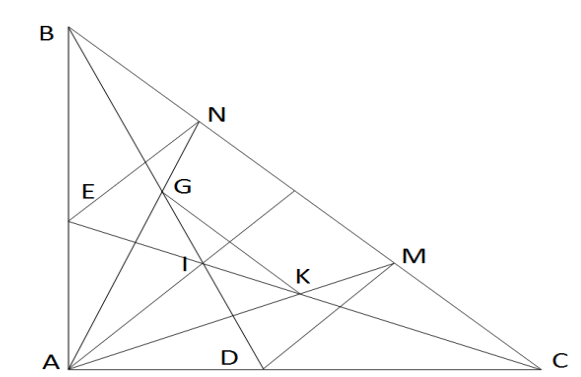
\includegraphics[width=0.55\textwidth]{10-4-lg.png}$$
		\begin{enumerate}
			\item $\triangle A B D=\triangle M B D($ cạnh huyền - góc nhọn $)\\
			=>\mathrm{AB}=\mathrm{AM}=>\triangle A M B$ cân ở B.
			\item Ta có $\triangle A E C=\triangle N E C=>\mathrm{CN}=\mathrm{CA} \\
			\mathrm{Khi} \text { đó } \mathrm{AB}+\mathrm{AC}=\mathrm{BM}+\mathrm{CN}=\mathrm{BM}+\mathrm{MC}+\mathrm{MN}=\mathrm{BC}+\mathrm{MN}
			\\ \quad \Rightarrow \mathrm{MN}=\mathrm{AB}+\mathrm{AC}-\mathrm{BC}$
			\item Từ $\triangle A M B$ cân ở $\mathrm{M} \Rightarrow A M B=\frac{180^{\circ}-A B C}{2}=90^{\circ}-\frac{A B C}{2}$\\
			Từ $\triangle A N C$ cân ở $\mathrm{N} \Rightarrow A N B=\frac{180^{\circ}-A C B}{2}=90^{\circ}-\frac{A C B}{2}$\\
			Trong $\triangle A M N$ có $M A N=180^{\circ}-A M B-A N C$\\
			$=180^{\circ}-\left(90^{\circ}-\frac{A B C}{2}\right)-\left(90^{\circ}-\frac{A C B}{2}\right)$\\
			$=\frac{A B C}{2}+\frac{A C B}{2}=\frac{90^{\circ}}{2}=45^{\circ}$
			(Vì $\triangle A B C$ vuông tại A nên $A B C+A C B=90^{\circ}$ )\\
			Vậy $M A N=45^{\circ}$
			\item Vì $\triangle A M B$ cân ở $\mathrm{B}$ nên đường phân giác $\mathrm{BD}$ đồng thời là đường cao $\Rightarrow B D \perp A M$ hay $G I \perp A K$\\
			$\triangle A N C$ cân ở $\mathrm{C} \Rightarrow$ đường phân giác $\mathrm{CE}$ đồng thời là đường cao $\Rightarrow C E \perp A N$ hay $K I \perp A G$\\ Trong $\triangle A K G$ có 2 đường cao xuất phát từ $\mathrm{G}, \mathrm{K}$ cắt nhau ở $\mathrm{I} \Rightarrow \mathrm{I}$ là trực tâm của $\triangle A K G$.\\ 
			$A I \perp G K$ ở $\mathrm{H} \Rightarrow A H G=90^{\circ}$
		\end{enumerate}
	}
\end{bt}

	\onehalfspacing
\section{Đề số 11}

\begin{bt} 
    \hfill
	\begin{enumerate}[a.]
		\item Tính giá trị của biểu thức: $A=\frac{4}{9}:\left(\frac{1}{15}-\frac{2}{3}\right)+\frac{4}{9}:\left(\frac{1}{11}-\frac{5}{22}\right)$
        \item Tìm $x$, biết: $\left(-1 \frac{3}{5}+x\right): \frac{12}{13}=2 \frac{1}{6}$
        \item Tính giá trị của biểu thức $M=21 x^2 y+4 x y^2$ với $x$, $y$ thoả mãn:
        $$
        (x-2)^4+(2 y-1)^{2014} \leq 0
        $$
	\end{enumerate}
	\loigiai{} 
\end{bt}

\begin{bt}
	\hfill
	\begin{enumerate}[a.]
		\item Tìm các số $\mathrm{x}, \mathrm{y}, \mathrm{z}$ biết: $\frac{x}{3}=\frac{y}{4} ; \quad \frac{y}{6}=\frac{z}{8} \quad$ và $2 x+y-z=-14$.
        \item Tìm $x$, biết: $(x-2)\left(x+\frac{2}{3}\right)>0$.
        \item Tìm số nguyên $x$, biết rằng: $\frac{3}{7} \cdot 15 \frac{1}{3}+\frac{3}{7} \cdot 5 \frac{2}{5} \leq x \leq\left(3 \frac{1}{2}: 7-6 \frac{1}{2}\right) \cdot\left(-2 \frac{1}{3}\right)$
	\end{enumerate}
	\loigiai{} 
\end{bt}

\begin{bt}
	\hfill
	\begin{enumerate}[a.]
		\item Tính giá trị của biểu thức $\mathrm{M}=4 \mathrm{x}+4 \mathrm{y}+21 \mathrm{xy}(\mathrm{x}+\mathrm{y})+7\left(\mathrm{x}^3 \mathrm{y}^2+\mathrm{x}^2 \mathrm{y}^3\right)+2014$, biết $\mathrm{x}+\mathrm{y}=0$.
        \item Cho đa thức $p(x)=a x^3+b x^2+c x+d$, với $a, b, c, d$ là các hệ số nguyên. Biết rằng, $\mathrm{p}(\mathrm{x}) \vdots 5$ với mọi $\mathrm{x}$ nguyên. Chứng minh rằng $\mathrm{a}, \mathrm{b}, \mathrm{c}, \mathrm{d}$ đều chia hết cho 5 .
        \item Cho $A=1+\frac{1}{2}+\frac{1}{3}+\frac{1}{4}+\ldots+\frac{1}{4026}, B=1+\frac{1}{3}+\frac{1}{5}+\frac{1}{7}+\ldots+\frac{1}{4025}$. So sánh $\frac{A}{B}$ với $1 \frac{2013}{2014}$.
	\end{enumerate}
	\loigiai{} 
\end{bt}

\begin{bt}
	Cho tam giác $A B C$ cân tại $A$. Trên cạnh $B C$ lấy điểm $D$ ( $D$ khác $B, C$ ). Trên tia đối của tia $C B$, lấy điểm $\mathrm{E}$ sao cho $\mathrm{CE}=\mathrm{BD}$. Đường vuông góc với $\mathrm{BC}$ kẻ từ $\mathrm{D}$ cắt $\mathrm{BA}$ tại $\mathrm{M}$. Đường vuông góc với $\mathrm{BC}$ kẻ từ $\mathrm{E}$ cắt tia $\mathrm{AC}$ tại $\mathrm{N}$. $\mathrm{MN}$ cắt $\mathrm{BC}$ tại $\mathrm{I}$.
	\begin{enumerate}[a.]
		\item Chứng minh rằng: $\mathrm{DM}=\mathrm{EN}$.
        \item Chứng minh rằng $\mathrm{IM}=\mathrm{IN} ; \mathrm{BC}<\mathrm{MN}$.
        \item Gọi $\mathrm{O}$ là giao của đường phân giác góc $\mathrm{A}$ và đường thẳng vuông góc với $\mathrm{MN}$ tại $\mathrm{I}$. Chứng minh rằng: $\triangle B M O=\triangle C N O$. Từ đó suy ra điểm $\mathrm{O}$ cố định.
	\end{enumerate}
	\loigiai{}
\end{bt}

\begin{bt}
Cho tam giác $\mathrm{ABC}$ cân tại $\mathrm{A}$. Trên đường trung tuyến $\mathrm{BD}$ lấy điểm $\mathrm{E}$ sao cho $D A E=A B D$ (E nằm giữa $\mathrm{B}$ và $\mathrm{D}$ ). Chứng minh rằng $D A E=E C B$.
\loigiai{}
\end{bt}
	
\section{Đề số 12}
\graphicspath{{./img/}}
\begin{bt} 
    \hfill
	\begin{enumerate}[a.]
		\item Tìm $x$ biết: $\quad \frac{1}{2016}: 2015 x=-\frac{1}{2015}$.
        \item Tìm các giá trị nguyên của $n$ để phân số $\mathrm{M}=\frac{3 n-1}{n-1}$ có giá trị là số nguyên.
        \item Tính giá trị của biểu thức: $N=x y^2 z^3+x^2 y^3 z^4+x^3 y^4 z^5+\ldots+x^{2014} y^{2015} z^{2016}$ tại: $\mathrm{x}=-1 ; \mathrm{y}=-1 ; \mathrm{z}=-1$
	\end{enumerate}
	\loigiai{
		\begin{enumerate}
			\item $\frac{1}{2016}: 2015 x=-\frac{1}{2015} \\
				  \frac{1}{2016.2015} x=\frac{-1}{2015} \\
				  x=\frac{-1}{2015}: \frac{1}{2016.2015}=-2016 \\
				  \text {Vậy } x=-2016$
			\item $\mathrm{M}=\frac{3 n-1}{n-1}$ có giá trị là số nguyên $\Rightarrow 3 n-1 \vdots n-1$\\
			$\Rightarrow 3(n-1)+2 \vdots n-1 \Rightarrow 2 \vdots n-1 \Rightarrow n-1 \in U^{\prime}(2)=\{-1 ; 1 ;-2 ; 2\}$\\
			Ta có bảng:\\ 
			\begin{table}[h]
				\begin{tabular}{lllll}
				\multicolumn{1}{l|}{n-1} & -1 & 1 & -2 & 2 \\ \hline
				\multicolumn{1}{l|}{n}   & 0  & 2 & -1 & 3 \\
				\end{tabular}
				\end{table}
				\\
			Thử lại ta có $n \in\{0 ; 2 ;-1 ; 3\}$ thì $\mathrm{M}$ nhận giá trị nguyên.
			\item Ta có : $\mathrm{N}=\mathrm{xyz} \cdot \mathrm{yz}^2+\mathrm{x}^2 \mathrm{y}^2 \mathrm{z}^2 \cdot \mathrm{yz}^2+\mathrm{x}^3 \mathrm{y}^3 \mathrm{z}^3 \cdot \mathrm{yz}^2+\ldots+\mathrm{x}^{2014} \mathrm{y}^{2014} \mathrm{z}^{2014} \cdot \mathrm{yz}^2$\\ Thay $\mathrm{y}=1 ; \mathrm{z}=-1$ ta được:\\
			$N =-x y z-x^2 y^2 z^2-x^3 y^3 z^3-\ldots-x^{2014} y^{2014} z^{2014} \\
	        =-(x y z)-(x y z)^2-(x y z)^3-\ldots-(x y z)^{2014} .$\\
			Thay $x y z=-1$ được:\\
			$\mathrm{N}=1-1+1-1+\ldots+1-1=0 \\
			\text {Vậy } \mathrm{N}=0 .$
		\end{enumerate}
	} 
\end{bt}

\begin{bt}
	\hfill
	\begin{enumerate}[a.]
		\item Cho dãy tỉ số bằng nhau $\frac{2 b z-3 c y}{a}=\frac{3 c x-a z}{2 b}=\frac{a y-2 b x}{3 c}$. Chứng minh: $\frac{x}{a}=\frac{y}{2 b}=\frac{z}{3 c}$
        \item Tìm tất cả các số tự nhiên $m, n$ sao cho : $2^m+2015=|n-2016|+n-2016$.
	\end{enumerate}
	\loigiai{
		\begin{enumerate}
			\item
				$\frac{2 b z-3 c y}{a}=\frac{3 c x-a z}{2 b}=\frac{a y-2 b x}{3 c} \\
				\Leftrightarrow \frac{2 a b z-3 a c y}{a^2}=\frac{6 b c x-2 a b z}{4 b^2}=\frac{3 a c y-6 b c x}{9 c^2} \\
				= \frac{2 a b z-3 a c y+6 b c x-2 a b z+3 a c y-6 b c x}{a^2+4 b^2+9 c^2}=0 \\
				\Rightarrow 2 b z-3 c y=0 \Rightarrow \frac{z}{3 c}=\frac{y}{2 b}(1) \\
				\Rightarrow 3 c x-a z=0 \Rightarrow \frac{x}{a}=\frac{z}{3 c}(2) ; \text { Từ (1) và (2) suy ra: } \frac{x}{a}=\frac{y}{2 b}=\frac{z}{3 c}$
			\item Nhận xét:\\
			$\text {-Với } x \geq 0 \text { thì }|x|+x=2 x \\
			\text {-Với } x<0 \text { thì }|x|+x=0 \text {. }$\\
			Do đó $|\mathrm{x}|+\mathrm{x}$ luôn là số chẵn với $\forall \mathrm{x} \in \mathrm{Z}$.\\
			Áp dụng nhận xét trên thì $|n-2016|+\mathrm{n}-2016$ là số chẵn với $\mathrm{n}-2016 \in \mathrm{Z}$.\\
            Suy ra $2^{\mathrm{m}}+2015$ là số chẵn $\Rightarrow 2^{\mathrm{m}}$ lẻ $\Leftrightarrow \mathrm{m}=0$.\\
            Khi đó $|\mathrm{n}-2016|+\mathrm{n}-2016=2016$\\
            + Nếu $\mathrm{n}<2016$, ta có - $(\mathrm{n}-2016)+\mathrm{n}-2016=2016 \Leftrightarrow 0=2016$ (loại)\\
            + Nếu $n \geq 2016$, ta có $2(n-2016)=2016 \Leftrightarrow n-2016=1008 \Leftrightarrow n=3024$ (thỏa mãn)\\
            Vậy $(m ; n)=(0 ; 3024)$
		\end{enumerate}
	} 
\end{bt}

\begin{bt}
	\hfill
	\begin{enumerate}[a.]
		\item Tìm giá trị nhỏ nhất của biểu thức $\mathrm{P}=|x-2015|+|x-2016|+|x-2017|$.
        \item Cho bốn số nguyên dương khác nhau thỏa mãn tổng của hai số bất kì chia hết cho 2 và tổng của ba số bất kì chia hết cho 3 . Tính giá trị nhỏ nhất của tổng bốn số này ?
	\end{enumerate}
	\loigiai{
		\begin{enumerate}
			\item $\mathrm{P}=|x-2015|+|2016-x|+|x-2017|=(|x-2015|+|2017-x|)+|x-2016|$\\
			Ta có: $|x-2015|+|2017-x| \geq|x-2015+2017-x|=2$. Dấu "=" xảy ra khi: $2015 \leq x \leq 2017$ (1)\\
			Lai có: $|x-2016| \geq 0$.\\ 
			Dấu "=" xảy ra khi $\mathrm{x}=2016$ (2).\\
			Từ (1) và (2) ta có $\mathrm{minP}=2$. Dấu " $=$ " xảy ra khi $x=2016$
			\item Nhận xét : Bốn số phải có cùng số dư khi chia cho 2 và 3 . Để có tổng nhỏ nhất, mỗi trong hai số dư này là 1 .\\
			Từ đó ta có các số $1,7,13$ và 19 . Tổng của chúng là : $1+7+13+19=40$.
		\end{enumerate}
	}
\end{bt}

\begin{bt}
    Cho tam giác $\mathrm{ABC}$ cân tại $\mathrm{A}, \mathrm{BH}$ vuông góc $\mathrm{AC}$ tại $\mathrm{H}$. Trên cạnh $\mathrm{BC}$ lấy điểm $M$ bất kì ( khác $B$ và $C$ ). Gọi $D, E, F$ là chân đường vuông góc hạ từ $M$ đến $A B, A C$, $\mathrm{BH}$.
    \begin{enumerate}
        \item Chứng $\operatorname{minh} \triangle \mathrm{DBM}=\triangle \mathrm{FMB}$.
        \item Chứng minh khi $\mathrm{M}$ chạy trên cạnh $\mathrm{BC}$ thì tổng $\mathrm{MD}+\mathrm{ME}$ có giá trị không đổi.
        \item Trên tia đối của tia $C A$ lấy điểm $\mathrm{K}$ sao cho $\mathrm{CK}=\mathrm{EH}$. Chứng minh $\mathrm{BC}$ đi qua trung điểm của DK.
    \end{enumerate}
\loigiai{
	$$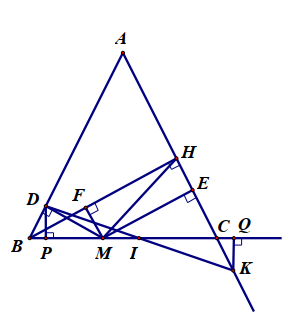
\includegraphics[width=0.4\textwidth]{12-4-lg.png}$$
	\begin{enumerate}
		\item $\text {Chứng minh được } \Delta \mathrm{DBM}=\Delta \mathrm{FMB} \text { (ch-gn) }$
		\item Theo câu a ta có: $\Delta \mathrm{DBM}=\Delta \mathrm{FMB}($ ch-gn $) \Rightarrow \mathrm{MD}=\mathrm{BF}$ (2 cạnh tương ứng)\\
		+) Chứng minh: $\Delta \mathrm{MFH}=\Delta \mathrm{HEM} \Rightarrow \mathrm{ME}=\mathrm{FH}$ (2 cạnh tương ứng)
		$(2)$\\
		Từ (1) và (2) suy ra: $\mathrm{MD}+\mathrm{ME}=\mathrm{BF}+\mathrm{FH}=\mathrm{BH}$\\
		BH không đổi $\Rightarrow \mathrm{MD}+\mathrm{ME}$ không đổi (đpcm)
		\item Vẽ $D P \perp B C$ tại $P, K Q \perp B C$ tại $Q$, gọi I là giao điểm của $D K$ và $B C$\\
		+) Chứng minh : $\mathrm{BD}=\mathrm{FM}=\mathrm{EH}=\mathrm{CK}$\\
		+) Chứng minh : $\triangle \mathrm{BDP}=\triangle \mathrm{CKQ}$ (ch-gn) $\Rightarrow \mathrm{DP}=\mathrm{KQ}$ (cạnh tương ứng)\\
		$+)$ Chứng minh: $\mathrm{IDP}=\mathrm{IKQ} \Rightarrow \Delta \mathrm{DPI}=\Delta \mathrm{KQI}(\mathrm{g}-\mathrm{c}-\mathrm{g}) \Rightarrow \mathrm{ID}=\mathrm{IK}$(đpcm)\\
	\end{enumerate}
}
\end{bt}

\begin{bt}
   Có sáu túi lân lượt chứa $18,19,21,23,25$ và $34$ bóng. Một túi chỉ chứa bóng đỏ trong khi năm túi kia chỉ chứa bóng xanh. Bạn Toán lấy ba túi, bạn Học lấy hai túi. Túi còn lại chứa bóng đỏ. Biết lúc này bạn Toán có số bóng xanh gấp đôi số bóng xanh của bạn Học. Tìm số bóng đỏ trong túi còn lại.
\loigiai{
	Tông số bóng trong 6 túi là : $18+19+21+23+25+34=140$
    Vì số bóng của Toán gấp hai lần số bóng của học nên tổng số bóng của hai bạn là bội của 3 . Ta có : 140 chia 3 bằng 46 dư 2. Do đó số bóng đỏ cũng là số chia 3 dư 2 .\\
    Trong sáu số đã cho chỉ có 23 chia 3 dư 2, đó chính là số bóng đỏ trong túi còn lại. Từ đó ta tìm được số bóng của Toán là : $18+21=39$. Số bóng của học là : $19+25+34=78$.
}
\end{bt}
	\onehalfspacing
\section{Đề số 13}
\graphicspath{{./img/}}
\begin{bt} 
    \hfill
	\begin{enumerate}[a.]
		\item $\left|x+\frac{1}{5}\right|-4=-2$
        \item $2 x-\frac{1}{5}=\frac{6}{5} x-\frac{1}{2}$
        \item $(x-3)^{x+2}-(x-3)^{x+8}=0$
	\end{enumerate}
	\loigiai{
        \begin{enumerate}
            \item Ta có:\\
            $\left|x+\frac{1}{5}\right|-4=-2 \Leftrightarrow\left|x+\frac{1}{5}\right|=2 \Leftrightarrow {\left[\begin{array} { l } 
            { x + \frac { 1 } { 5 } = 2 } \\
            { x + \frac { 1 } { 5 } = - 2 }
            \end{array} \Leftrightarrow \left[\begin{array}{l}
            x=\frac{9}{5} \\
            x=-\frac{11}{5}
            \end{array}\right.\right.} \\
            \text {Vậy với } x=\frac{9}{5} \text { hoặc } x=-\frac{11}{5} \text { thì }\left|x+\frac{1}{5}\right|-4=-2$
            \item Ta có:
            $
            2 x-\frac{1}{5}=\frac{6}{5} x-\frac{1}{2} \Leftrightarrow \frac{4}{5} x=-\frac{3}{10} \Rightarrow x=-\frac{3}{8}
            $
            \item Ta có: $(x-3)^{x+2}-(x-3)^{x+8}=0 \Leftrightarrow(x-3)^{x+2}\left[1-(x-3)^6\right]=0$
            $\\
            \Leftrightarrow\left[\begin{array} { l } 
            { x - 3 = 0 } \\
            { ( x - 3 ) ^ { 6 } = 1 }
            \end{array} \Leftrightarrow \left[\begin{array}{l}
            x=3 \\
            x=4 \\
            x=2
            \end{array}\right.\right.
            $
        \end{enumerate}
    } 
\end{bt}

\begin{bt}
	Tìm $x, y, z$ biết $\frac{x}{2}=\frac{y}{3}=\frac{z}{4}$ và $x^2+y^2+z^2=116$
	\loigiai{
            $\frac{x}{2}=\frac{y}{3}=\frac{z}{4} \Rightarrow \frac{x^2}{4}=\frac{y^2}{9}=\frac{z^2}{16}=\frac{x^2+y^2+z^2}{4+9+16}=\frac{116}{29}=4 \\[10pt]
            \Rightarrow \frac{x^2}{4}=\frac{y^2}{9}=\frac{z^2}{16}=4 \Rightarrow \frac{x}{2}=\frac{y}{3}=\frac{z}{4}= \pm 2 \\[10pt]
            \text {Vậy }(x ; y ; z)=(4 ; 6 ; 8) \text { hoặc }(x ; y ; z)=(-4 ;-6 ;-8)$
    } 
\end{bt}

\begin{bt}
	Trong vòng bán kết giải bóng đá của trường THCS Phù Đổng có 4 đội thi đấu, gọi $\mathrm{A}$ là tập hợp các cầu thủ; B là tập hợp các số áo thi đấu. Quy tắc mỗi cầu thủ ứng với số áo của họ có phải là một hàm số không? Vì sao?
	\loigiai{
        Quy tắc mỗi cầu thủ ứng với số áo của họ không là một hàm số vì đại lượng cầu thủ không phải là các giá trị bằng số. (trả lời đúng giải thích sai không có điểm)
    }
\end{bt}

\begin{bt}
    Tính giá trị của đa thức $\mathrm{P}=x^3+x^2 y-2 x^2-x y-y^2+3 y+x+2017$ với
    $
    x+y=2
    $
\loigiai{
        $P=x^3+x^2 y-2 x^2-x y-y^2+3 y+x+2017 \\[7pt]
        =x^2(x+y)-2 x^2-y(x+y)+3 y+x+2017 \\[7pt]
        =2 x^2-2 x^2-2 y+3 y+x+2017=x+y+2017=2019 \\[7pt]
        \text {Vậy với } x+y=2 \text { thì } P=2019\\[7pt]
        \text { Hoặc nhóm để xuất hiện } \mathrm{x}+\mathrm{y} \text { - } 2$
}
\end{bt}

\begin{bt}
    Cho : $\frac{3 x-2 y}{4}=\frac{2 z-4 x}{3}=\frac{4 y-3 z}{2}$. Chứng minh: $\frac{x}{2}=\frac{y}{3}=\frac{z}{4}$
\loigiai{
        $\frac{3 x-2 y}{4}=\frac{2 z-4 x}{3}=\frac{4 y-3 z}{2} \\[7pt]
        \Rightarrow \frac{12 x-8 y}{16}=\frac{6 z-12 x}{9}=\frac{8 y-6 z}{4}=\frac{12 x-8 y+6 z-12 x+8 y-6 z}{16+9+4}=0 \\[7pt]
        \Rightarrow 12 x=8 y=6 z \Rightarrow \frac{12 x}{24}=\frac{8 y}{24}=\frac{6 z}{24} \\[7pt]
        \Rightarrow \frac{x}{2}=\frac{y}{3}=\frac{z}{4}$
}
\end{bt}

\begin{bt}
    Tìm các số tự nhiên $\mathrm{x}$, $y$ thỏa mãn: $2 \mathrm{x}^2+3 \mathrm{y}^2=77$  
\loigiai{
    $2 x^2+3 y^2=77 \Rightarrow 3 y^2=77-2 y^2 \leq 77 \Rightarrow y^2 \leq 77 / 3 \Rightarrow y^2 \leq 25$\\[6pt]
    Mà $2 x^2$ chẵn; 77 lẻ $\Rightarrow 3 y^2$ lẻ $\Rightarrow y^2$ lẻ $\Rightarrow y^2 \in\{1 ; 9 ; 25\}$\\[6pt]
    $+y^2=1 \Rightarrow 2 x^2=77-3=74 \Rightarrow x^2=37 \Rightarrow \text { không có số tự nhiên } \mathrm{x} \\[6pt]
    +y^2=9 \Rightarrow 2 x^2=77-27=50 \Rightarrow x^2=25 \Rightarrow x=5 \text { và } y=3 \\[6pt]
    +y^2=25 \Rightarrow 2 x^2=77-75=2 \Rightarrow x^2=1 \Rightarrow x=1 \text { và } y=5$\\[6pt]
    Vậy số tự nhiên $x$, $y$ thỏa mãn $2 x^2+3 y^2=77$ là $(x ; y)=(5 ; 3) ;(1 ; 5)$\\[6pt]
    Học sinh lân lượt thư chọn các số tụ nhiên $x$ (hoặc y) từ $0,1,2, \ldots$ để có được KQ sẽ không được điểm vì không thể hiện được năng lực tu duy số học.
}
\end{bt}

\begin{bt}
    Cho $\triangle \mathrm{ABC}$, tia phân giác của góc $\mathrm{A}$ cắt $\mathrm{BC}$ tại $\mathrm{D}$. Biết $\mathrm{ADB}=85^{\circ}$
    \begin{enumerate}
        \item Tính: $\mathrm{B}-\mathrm{C}$
        \item Tính các góc của $\triangle \mathrm{ABC}$ nếu $4 . B=5 . C$
    \end{enumerate}
\loigiai{
    $$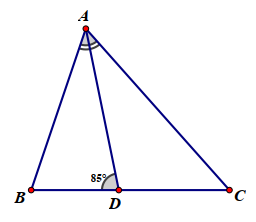
\includegraphics[width=0.4\textwidth]{13-4-lg.png}$$
    \begin{enumerate}
        \item Xét $\triangle \mathrm{ADC}$ có $\mathrm{ADB}$ là góc ngoài tại $\mathrm{D}$\\[5pt]
        $\Rightarrow \mathrm{ADB}=\mathrm{C}+\mathrm{DAC}=85^{\circ}$\\[5pt]
        Xét $\triangle \mathrm{ADB}$ có $\mathrm{ADC}$ là góc ngoài tại $\mathrm{D}$
        $\Rightarrow \mathrm{ADC}=\mathrm{B}+\mathrm{BAD}=180^{\circ}-85^{\circ}=95^{\circ}$\\[5pt]
        Mà $\mathrm{DAC}=\mathrm{BAD}(\mathrm{Vi} \mathrm{AD}$ là tia phân giác của góc $\mathrm{A})$\\[5pt] 
        $\Rightarrow$ Từ $(1)$ và $(2) \Rightarrow \mathrm{B}-\mathrm{C}=95^{\circ}-85^{\circ}=10^{\circ}$
        \item Vì $\mathrm{B}-\mathrm{C}=10^{\circ}$ mà $4 \cdot \mathrm{B}=5 \cdot \mathrm{C} \Rightarrow \frac{\mathrm{B}}{5}=\frac{\mathrm{C}}{4}=\frac{\mathrm{B}-\mathrm{C}}{5-4}=10^{\circ}$\\[5pt] 
        $\Rightarrow B=50^{\circ}$ và $C=40^{\circ} \Rightarrow A=90^{\circ}$
    \end{enumerate}
}
\end{bt}

\begin{bt}
    Cho $\triangle \mathrm{ABC}$ có ba góc nhọn, trung tuyến $\mathrm{AM}$. Trên nửa mặt phẳng bờ $\mathrm{AB}$ chứa điểm $\mathrm{C}$, vẽ đoạn thẳng $\mathrm{AE}$ vuông góc và bằng $\mathrm{AB}$. Trên nửa mặt phẳng bờ $\mathrm{AC}$ chứa điểm $B$, vẽ đoạn thẳng $A D$ vuông góc và bằng $A C$.

\begin{enumerate}
    \item Chứng minh: $\mathrm{BD}=\mathrm{CE}$
    \item Trên tia đối của tia MA lấy $\mathrm{N}$ sao cho $\mathrm{MN}=\mathrm{MA}$. Chứng minh: $\triangle \mathrm{ADE}=\Delta \mathrm{CAN}$.
    \item Gọi I là giao điểm của $\mathrm{DE}$ và $\mathrm{AM}$. Chứng minh: $\frac{\mathrm{AD}^2+\mathrm{IE}^2}{\mathrm{DI}^2+\mathrm{AE}^2}=1$
\end{enumerate}
\loigiai{
    $$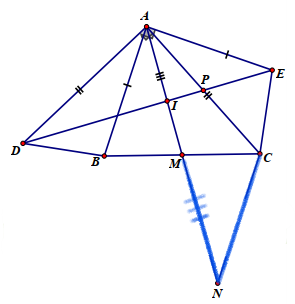
\includegraphics[width=0.4\textwidth]{13-5-lg.png}$$
    \begin{enumerate}
        \item Xét $\triangle \mathrm{ABD}$ và $\triangle \mathrm{ACE}$ có:\\[5pt]
        $\mathrm{AD}=\mathrm{AC}(\mathrm{gt}) \\[5pt]
        \mathrm{AE}=\mathrm{AB}(\mathrm{gt})$ \\[5pt]
        $\mathrm{BAD}=\mathrm{CAE}$ (Cùng phụ với $\mathrm{BAC}$ )\\[5pt] 
        $\Rightarrow \triangle \mathrm{ABD}=\triangle \mathrm{AEC} \text { (c.g.c) } \\[5pt]
        \Rightarrow \mathrm{BD}=\mathrm{CE} \text { (Hai cạnh tương ứng) }$
        \item Xét $\triangle \mathrm{ABM}$ và $\triangle \mathrm{NCM}$ có $\mathrm{AM}=\mathrm{MN}$ (gt); $\mathrm{BM}=\mathrm{CM}$ (gt) $\mathrm{AMB}=\mathrm{AMC}$
        (đối đỉnh)\\[5pt]
        $\Rightarrow \triangle \mathrm{ABM}=\Delta \mathrm{NCM}$ (c.g.c)\\[5pt] 
        $\Rightarrow \mathrm{AB}=\mathrm{CN}$ (hai cạnh tương ứng), $A B M=N C M$ (Hai góc tương ứng)\\[4pt]
        Ta có $\mathrm{ACN}=\mathrm{ACB}+\mathrm{BCN}=\mathrm{ACB}+\mathrm{ABC}=180^{\circ}-\mathrm{BAC}$\\[4pt]
        Lại có $\mathrm{DAE}=\mathrm{DAC}+\mathrm{BAE}-\mathrm{BAC}=180^{\circ}-\mathrm{BAC}$\\[5pt]
        $\Rightarrow \mathrm{DAE}=\mathrm{ACN}$\\[4pt]
        Xét $\triangle \mathrm{ADE}$ và $\triangle \mathrm{ACN}$ có $\mathrm{CN}=\mathrm{AE}$ (cùng bằng $\mathrm{AB}$ )\\[5pt]
        $\mathrm{AC}=\mathrm{AD}(\mathrm{gt})$
        $\mathrm{DAE}=\mathrm{ACN} (\mathrm{cmt}) \\[4pt]
        \Rightarrow \triangle \mathrm{ADE}=\triangle \mathrm{CAN} \text { (c.g.c) }$
        \item  $\text{Vì } \triangle \mathrm{ADE}=\Delta \mathrm{CAN}(\mathrm{cmt}) \Rightarrow \mathrm{NAC}=\mathrm{ADE}$ (Hai góc tương ứng)\\[5pt]
        Gọi $P$ là giao điểm của $\mathrm{DE}$ và $\mathrm{AC}$\\[5pt]
        Xét $\triangle \mathrm{ADP}$ vuông tại $\mathrm{A} \Rightarrow \mathrm{ADE}+\mathrm{APD}=90^{\circ} \Rightarrow \mathrm{NAC}+\mathrm{APD}=90^{\circ}$ $\Rightarrow \mathrm{AI} \perp \mathrm{DE}$\\[5pt]
        Xét $\triangle \mathrm{ADI}$ vuông tại I. Theo ĐL Pytago ta có $\mathrm{AD}^2=\mathrm{DI}^2+\mathrm{AI}^2 \Rightarrow \mathrm{AI}^2=\mathrm{AD}^2-\mathrm{DI}^2$\\[5pt] Xét $\triangle \mathrm{AIE}$ vuông tại I. Theo ĐL Pytago ta có $\mathrm{AE}^2=\mathrm{AI}^2+\mathrm{IE}^2 \Rightarrow \mathrm{AI}^2=\mathrm{AE}^2-\mathrm{IE}^2$\\[5pt] $\Rightarrow \mathrm{AD}^2-\mathrm{DI}^2=\mathrm{AE}^2-\mathrm{IE}^2 \Rightarrow \mathrm{AD}^2+\mathrm{IE}^2=\mathrm{DI}^2+\mathrm{AE}^2 \Rightarrow \frac{\mathrm{AD}^2+\mathrm{IE}^2}{\mathrm{DI}^2+\mathrm{AE}^2}=1$(đpcm)
    \end{enumerate}
}
\end{bt}
	\onehalfspacing
\section{Đề số 14}

\begin{bt} 
    \hfill
	\begin{enumerate}[a.]
		\item Cho biểu thức: $\mathrm{P}=\mathrm{x}-4 \mathrm{xy}+\mathrm{y}$. Tính giá trị của $\mathrm{P}$ với $|x|=1,5 ; \mathrm{y}=-0,75$
        \item Rút gọn biểu thức: $\mathrm{A}=\frac{2^{12} \cdot 3^5-4^6 \cdot 81}{\left(2^2 \cdot 3\right)^6+8^4 \cdot 3^5}$
	\end{enumerate}
	\loigiai{} 
\end{bt}

\begin{bt}
	\hfill
	\begin{enumerate}[a.]
		\item Tìm $x, y, z$, biết:
        $$
        2 x=3 y ; 4 y=5 z \text { và } x+y+z=11
        $$
        \item Tìm $x$, biết: $|x+1|+|x+2|+|x+3|=4 x$
	\end{enumerate}
	\loigiai{} 
\end{bt}

\begin{bt}
	Cho hàm số: $\mathrm{y}=\mathrm{f}(\mathrm{x})=-4 \mathrm{x}^3+\mathrm{x}$
	\begin{enumerate}[a.]
		\item Tính $f(0), f(-0,5)$
        \item Chứng minh: $f(-a)=-f(a)$.
	\end{enumerate}
	\loigiai{}
\end{bt}

\begin{bt}
    Tìm cặp số nguyên $(x ; y)$ biết: $\quad x+y=x \cdot y$
\loigiai{}
\end{bt}

\begin{bt}
    Câu 5(6 điêm): Cho $\triangle \mathrm{ABC}$ có góc $\mathrm{A}$ nhỏ hơn $90^{\circ}$. Vẽ ra ngoài tam giác $\mathrm{ABC}$ các tam giác vuông cân tại $\mathrm{A}$ là $\triangle \mathrm{ABM}$ và $\triangle \mathrm{ACN}$.
    \begin{enumerate} 
        \item Chứng minh rằng: $\triangle \mathrm{AMC}=\triangle \mathrm{ABN}$;
        \item Chứng minh: $\mathrm{BN} \perp \mathrm{CM}$;
        \item Kẻ $\mathrm{AH} \perp \mathrm{BC}(\mathrm{H} \in \mathrm{BC})$. Chứng minh $\mathrm{AH}$ đi qua trung điểm của $\mathrm{MN}$.
    \end{enumerate}
\loigiai{}
\end{bt}

\begin{bt}
    Cho ba số $\mathrm{a}, \mathrm{b}, \mathrm{c}$ thõa mãn: $0 \leq a \leq b+1 \leq c+2$ và $\mathrm{a}+\mathrm{b}+\mathrm{c}=1$. Tìm giá trị nhỏ nhất của c.
\loigiai{}
\end{bt}
	\onehalfspacing
\section{Đề số 15}
\graphicspath{{./img/}}
\begin{bt} 
    \hfill
	\begin{enumerate}[a.]
		\item Thực hiện phép tính:
        $$
        \mathrm{A}=\frac{9 \cdot 6^9 \cdot 120-4^6 \cdot 9^6}{8^4 \cdot 3^{13}-6^{12}} ; \quad \mathrm{B}=\frac{10}{7 \cdot 12}+\frac{10}{12 \cdot 17}+\frac{10}{17 \cdot 22}+\ldots+\frac{10}{2012 \cdot 2017}+\frac{10}{2017 \cdot 2022}
        $$
        \item Cho a, b, c là ba số thực khác 0 , thoả mãn : $\frac{a+b-c}{c}=\frac{b+c-a}{a}=\frac{a+c-b}{b}$.
        Hãy tính giá trị của biểu thức $B=\left(1+\frac{b}{a}\right) \cdot\left(1+\frac{a}{c}\right) \cdot\left(1+\frac{c}{b}\right)$.
        \item Tính giá trị của đa thức $f(x)=x^5-2018 x^4+2016 x^3+2018 x^2-2016 x-2017$ tại $x=2017$
	\end{enumerate}
	\loigiai{
        \begin{enumerate}
            \item $A=\frac{9 \cdot 6^9 \cdot 120-4^6 \cdot 9^6}{8^4 \cdot 3^{12}-6^{12}}=\frac{3^2 \cdot 2^9 \cdot 3^9 \cdot 2^3 \cdot 3 \cdot 5-2^{12} \cdot 3^{12}}{2^{12} \cdot 3^{13}-2^{12} \cdot 3^{12}} \triangleleft \\[5pt]
            =\frac{3^{12} \cdot 2^{12} \cdot 5-2^{12} \cdot 3^{12}}{2^{12} \cdot 3^{12}(3-1)}=\frac{3^{12} \cdot 2^{12}(5-1)}{2^{12} \cdot 3^{12} \cdot 2} \\[5pt]
            =\frac{5-1}{2}=2 \\[5pt]
            \text { Vậy } A=2 \\[5pt]
            B=\frac{10}{7 \cdot 12}+\frac{10}{12 \cdot 17}+\frac{10}{17 \cdot 22}+\ldots+\frac{10}{2012 \cdot 2017}+\frac{10}{2017 \cdot 2022} \\[5pt]
            =2 \cdot\left(\frac{5}{7 \cdot 12}+\frac{5}{12 \cdot 17}+\frac{5}{17 \cdot 22}+\ldots .+\frac{5}{2012 \cdot 2017}+\frac{5}{2017 \cdot 2022}\right) \\[5pt]
            =2\left(\frac{1}{7}-\frac{1}{12}+\frac{1}{12}-\frac{1}{17}+\frac{1}{17}-\frac{1}{22}+\ldots .+\frac{1}{2012}-\frac{1}{2017}+\frac{1}{2017}-\frac{1}{2022}\right) \\[5pt]
            =2\left(\frac{1}{7}-\frac{1}{2022}\right)=2 \cdot \frac{2022-7}{2022 \cdot 7}=\frac{2015}{7077} \\[5pt]
            \text { Vậy } B=\frac{2015}{7077}$
            \item +) Nếu a $+b+c \neq 0$\\[5pt]
            Theo tính chất dãy tỉ số bằng nhau, ta có:\\[5pt]
            $\frac{a+b-c}{c}=\frac{b+c-a}{a}=\frac{c+a-b}{b}=\frac{a+b-c+b+c-a+c+a-b}{a+b+c}=1 \\[5pt]
            \text { mà } \frac{a+b-c}{c}+1=\frac{b+c-a}{a}+1=\frac{c+a-b}{b}+1=2 \\[5pt]
            \Rightarrow \frac{a+b}{c}=\frac{b+c}{a}=\frac{c+a}{b}=2 \\[5pt]
            \text { Vậy B }=\left(1+\frac{b}{a}\right)\left(1+\frac{a}{c}\right)\left(1+\frac{c}{b}\right)=\left(\frac{b+a}{a}\right)\left(\frac{c+a}{c}\right)\left(\frac{b+c}{b}\right)=8$\\[5pt]
            +) Nếu $a+b+c=0$\\[5pt]
            Theo tính chất dãy tỉ số bằng nhau, ta có:\\[5pt]
            $\frac{a+b-c}{c}=\frac{b+c-a}{a}=\frac{c+a-b}{b}=\frac{a+b-c+b+c-a+c+a-b}{a+b+c}=0\\[5pt]
            \text { mà } \frac{a+b-c}{c}+1=\frac{b+c-a}{a}+1=\frac{c+a-b}{b}+1=1 \\[5pt]
            \Rightarrow \frac{a+b}{c}=\frac{b+c}{a}=\frac{c+a}{b}=1 \\[5pt]
            \text { Vậy B }=\left(1+\frac{b}{a}\right)\left(1+\frac{a}{c}\right)\left(1+\frac{c}{b}\right)=\left(\frac{b+a}{a}\right)\left(\frac{c+a}{c}\right)\left(\frac{b+c}{b}\right)=1$
            \item Tính giá trị của đa thức:\\[5pt]
            $f(x)=x^5-2018 x^4+2016 x^3+2018 x^2-2016 x-2017$ tại $\mathrm{x}=2017$\\[5pt]
            Ta có $x=2017 \Rightarrow\left\{\begin{array}{l}2018=x+1 \\[5pt] 2016=x-1\end{array}\right.$.\\[5pt] 
            Khi đó ta có:\\[5pt]
            $f(2017) =x^5-(x+1) x^4+(x-1) x^3+(x+1) x^2-(x-1) x-x \\[5pt]
            =x^5-x^5-x^4+x^4-x^3+x^3+x^2-x^2+x-x
            = 0$\\[5pt]
            Vậy $f(2017)=0$
        \end{enumerate}
    } 
\end{bt}

\begin{bt}
    \hfill
    \begin{enumerate}
        \item Cho $\frac{3 x-2 y}{4}=\frac{2 z-4 x}{3}=\frac{4 y-3 z}{2}$. Chứng minh rằng : $\frac{x}{2}=\frac{y}{3}=\frac{z}{4}$.
        \item Tìm $x, y, z$ biết: $\quad\left|x-\frac{1}{2}\right|+\left|y+\frac{2}{3}\right|+\left|x^2+x z\right|=0$
    \end{enumerate}
    \loigiai{
    \begin{enumerate}
        \item Theo bài ra ta có: $\frac{3 x-2 y}{4}=\frac{2 z-4 x}{3}=\frac{4 y-3 z}{2}$\\[5pt]
        Áp dụng tính chất của dãy tỉ số bằng nhau ta có:\\[5pt]
        $\Rightarrow \frac{12 x-8 y}{16}=\frac{6 z-12 x}{9}=\frac{8 y-6 z}{4}=\frac{12 x-8 y+6 z-12 x+8 y-6 z}{16+9+4}=0 \\[5pt]
        \Rightarrow\left\{\begin{array} { l } 
        { 1 2 x - 8 y = 0 } \\
        { 8 y - 6 z = 0 }
        \end{array} \Rightarrow \left\{\begin{array}{l}
        12 x=8 y \\
        8 y=6 z
        \end{array} \Rightarrow 12 x=8 y=6 z\right.\right.\\[5pt]
        \Rightarrow \frac{12 x}{24}=\frac{8 y}{24}=\frac{6 z}{24}\\[8pt] \Leftrightarrow \frac{x}{2}=\frac{y}{3}=\frac{z}{4}(\mathrm{dpcm})$
        \item Áp dụng tính chất $|A| \geq 0$\\[5pt]
        $
        \Rightarrow\left\{\begin{array} { l } 
        { | x - \frac { 1 } { 2 } | = 0 } \\
        { | y + \frac { 2 } { 3 } | = 0 } \\
        { | x ^ { 2 } + x z | = 0 }
        \end{array} \Rightarrow \left\{\begin{array} { l } 
        { x - \frac { 1 } { 2 } = 0 } \\
        { y + \frac { 2 } { 3 } = 0 } \\
        { x ( x + z ) = 0 }
        \end{array} \Rightarrow \left\{\begin{array}{l}
        x=\frac{1}{2} \\
        y=-\frac{2}{3} \\
        z=-x=-\frac{1}{2}
        \end{array}\right.\right.\right.
        $\\[5pt]
        Vậy $\mathrm{x}=\frac{1}{2} ; \mathrm{y}=-\frac{2}{3} ; \mathrm{z}=-\frac{1}{2}$
    \end{enumerate}
        }
\end{bt}

\begin{bt}
	\hfill
	\begin{enumerate}[a.]
		\item Tìm các cặp số tự nhiên $(\mathrm{x} ; \mathrm{y})$ sao cho: $49-\mathrm{y}^2=12(\mathrm{x}-2001)^2$
        \item Cho $\left|2019 x_1-2018 y_1\right|+\left|2019 x_2-2018 y_2\right|+\ldots+\left|2019 x_{2018}-2018 y_{2018}\right| \leq 0$. Chứng minh
        $$
        \frac{x_1+x_2+x_3+\ldots+x_{2018}}{y_1+y_2+y_3+\ldots+y_{2018}}=\frac{2018}{2019} \text {. }
        $$
        \item Một cửa hàng có ba cuộn vải, tổng chiều dài ba cuộn vải đó là $186 \mathrm{~m}$, giá tiền mỗi mét vải của ba cuộn là như nhau. Sau khi bán được một ngày cửa hàng còn lại $\frac{2}{3}$ cuộn thứ nhất, $\frac{1}{3}$ cuộn thứ hai, $\frac{3}{5}$ cuộn thứ ba. Số tiền bán được của ba cuộn thứ nhất, thứ hai, thứ ba lần lượt tỉ lệ với $2 ; 3 ; 2$. Tính xem trong ngày đó cửa hàng đã bán được bao nhiêu mét vải mỗi cuộn.
	\end{enumerate}
	\loigiai{
        \begin{enumerate}
            \item Xét đẳng thức: $49-y^2=12(x-2001)^2$.\\[5pt]
            Vế phải là mộ số chẵn không âm nên y là một số lẻ và không lớn hơn 7.\\[5pt]
            Khi $\mathrm{y}=1 \Rightarrow \mathrm{x}=2003$ và $\mathrm{x}=1999$\\[5pt]
            Khi $y=3$ không có giá trị $x \in N$\\[5pt]
            Khi $y=5$ không có giá trị $x \in \mathrm{N}$\\[5pt]
            Khi $\mathrm{y}=7 \Rightarrow \mathrm{x}=2011$\\[5pt]
            Vậy các cặp (x; y) cần tìm là $(2003 ; 1) ;(1999 ; 1)$; (2001; 7)
            \item Ta có:\\[5pt]
            $\left|2019 x_1-2018 y_1\right| \geq 0 \\[5pt]
            \left|2019 x_2-2018 y_2\right| \geq 0 \\[5pt]
            \ldots \\[5pt]
            \left|2019 x_{2018}-2018 y_{2018}\right| \geq 0 \\[5pt]
            \Rightarrow\left(2017 x_1-2016 y_1\right)^2+\left(2017 x_2-2016 y_2\right)^2+\ldots+\left(2017 x_{2016}-2016 y_{2016}\right)^2 \geq 0$\\[5pt]
            Theo bài ra ta có:\\[5pt]
            $\left|2019 x_1-2018 y_1\right|+\left|2019 x_2-2018 y_2\right|+\ldots+\left|2019 x_{2018}-2018 y_{2018}\right| \leq 0$\\[5pt]
            Suy ra:\\[5pt]
            $\left\{\begin{array}{c}
            \left|2019 x_1-2018 y_1\right|=0 \\
            \left|2019 x_2-2018 y_2\right|=0 \\
            \vdots \\
            \left|2019 x_{2018}-2018 y_{2018}\right|=0
            \end{array}\right. \\
            \Rightarrow\left\{\begin{array}{c}
            2019 x_1=2018 y_1 \\
            2019 x_2=2018 y_2 \\
            \vdots \\
            2019 x_{2018}=2018 y_{18}
            \end{array}\\[5pt] \Rightarrow \frac{x_1}{y_1}=\frac{x_2}{y_2}=\ldots=\frac{x_{2018}}{y_{2018}}=\frac{2018}{2019}\right. \\[5pt]$
            Áp dụng tính chất của dãy tỉ số bằng nhau ta được:\\[5pt]
            $\frac{x_1}{y_1}=\frac{x_2}{y_2}=\ldots=\frac{x_{2018}}{y_{2018}}=\frac{x_1+x_2+\ldots+x_{2018}}{y_1+y_2+\ldots+y_{2018}} \\[5pt]
            \text {Từ (1) và (2) suy ra } \frac{x_1+x_2+x_3+\ldots+x_{2018}}{y_1+y_2+y_3+\ldots+y_{2018}}=\frac{2018}{2019}$(đpcm)
            \item Gọi chiều dài cuộn vải thứ nhât, thứ hai, thứ ba lần lượt là $x, y, z(m)$ ĐK: $0<x, y, z<186$\\[5pt]
            +) Tổng chiều dài ba cuộn vải đó là $186 \mathrm{~m} \Rightarrow \mathrm{x}+\mathrm{y}+\mathrm{z}=186$\\[5pt]
            +) Sau khi bán được một ngày cửa hàng còn lại $\frac{2}{3}$ cuộn thứ nhất, $\frac{1}{3}$ cuộn thứ hai, $\frac{3}{5}$ cuộn thứ ba\\[5pt]
            Trong ngày đó cửa hàng đã bán được số mét vải ở cuộn thứ nhất, thứ hai, thứ ba lần lượt là $\frac{x}{3}, \frac{2 y}{3}, \frac{2 z}{5}$ (mét)\\[5pt]
            +) Số tiền bán được của ba cuộn thứ nhất, thứ hai, thứ ba lần lượt tỉ lệ với 2; $3 ; 2$ và giá tiền mỗi mét vải của ba cuộn như nhau.\\[5pt]
            $\Rightarrow$ Số mét vải bán được của ba cuộn thứ nhất, thứ hai, thứ ba lần lượt tỉ lệ với 2; 3; 2\\[5pt]
            $\Rightarrow \frac{x}{3}: \frac{2 y}{3}: \frac{2 z}{5}=2: 3: 2 \Rightarrow \frac{2 x}{12}=\frac{2 y}{9}=\frac{2 z}{10}$\\[5pt]
            Áp dụng tính chất của dãy tỉ số bằng nhau ta được:\\[5pt] $\frac{x}{12}=\frac{y}{9}=\frac{z}{10}=\frac{x+y+z}{12+9+10}=\frac{186}{31}=6$\\[5pt]
            $\Rightarrow\left\{\begin{array}{l}
            x=72 \\
            y=54 \\
            z=60
            \end{array}\right. \text { (Thỏa mãn điều kiện) }$\\[5pt]
            Vậy trong ngày đó cửa hàng đã bán số mét vải ở cuộn thứ nhất, thứ hai, thứ ba lần lượt là : 24; 36; 24 (mét).
        \end{enumerate}
    } 
\end{bt}

\begin{bt}
	Cho tam giác $A B C, M$ là trung điểm của $B C$. Trên tia đối của của tia MA lấy điểm $\mathrm{E}$ sao cho $\mathrm{ME}=\mathrm{MA}$. Chứng minh rằng:
	\begin{enumerate}[a.]
		\item $\mathrm{AC}=\mathrm{EB}$ và $\mathrm{AC} / / \mathrm{BE}$
        \item Gọi I là một điểm trên $\mathrm{AC} ; \mathrm{K}$ là một điểm trên $\mathrm{EB}$ sao cho $\mathrm{AI}=\mathrm{EK}$. Chứng minh ba điểm I, M $\mathrm{K}$ thẳng hàng
        \item Từ E kẻ $E H \perp B C(H \in B C)$. Biết $H B E=50^{\circ} ; M E B=25^{\circ}$. Tính $H E M$ và $B M E$
    \end{enumerate}
	\loigiai{
        $$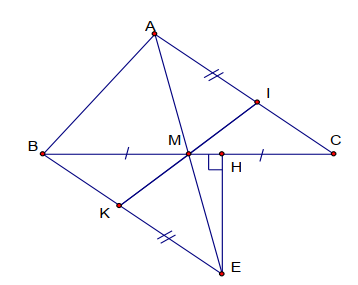
\includegraphics[width=0.5\textwidth]{15-4-lg.png}$$
        \begin{enumerate}
            \item Xét $\triangle A M C$ và $\triangle E M B$ có :
            $\mathrm{AM}=\mathrm{EM} \quad(\mathrm{gt}) \\[5pt]
            A M C=E M B \quad \text { (đối đỉnh }) \\[5pt]
            \mathrm{BM}=\mathrm{MC} \quad(\mathrm{gt}) \\[5pt]
            \text { Nên : } \triangle A M C=\Delta E M B \text { (c.g.c }) \\[5pt]
            \Rightarrow \mathrm{AC}=\mathrm{EB} \\[5pt]
            \text { Vì } \triangle A M C=\triangle E M B \\[5pt]\Rightarrow M A C=M E B$\\[5pt]
            Mà $M A C$ và $M E B$ là 2 góc có vị trí so le trong \\[5pt]Suy ra $\mathrm{AC} / / \mathrm{BE}$.
            \item Xét $\triangle A M I$ và $\triangle E M K$ có:\\[5pt]
            $\mathrm{AM}=\mathrm{EM}(\mathrm{gt}) \\[5pt]
            M A I=M E K \text { (vì } \triangle A M C=\triangle E M B) \\[5pt]
            \mathrm{AI}=\mathrm{EK} \text { (gt }) \\[5pt]
            \text { Nên } \triangle A M I=\Delta E M K(\text { c.g.c ) } \\[5pt]
            \text { Suy ra } A M I=E M K \\[5pt]
            \text { Mà } A M I+I M E=180^{\circ} \text { ( tính chất hai góc kề bù ) } \\[5pt]
            \Rightarrow \mathrm{EMK}+I M E=180^{\circ} \\[5pt]
            \Rightarrow \text { Ba điểm } \mathrm{I} ; \mathrm{M} ; \mathrm{K} \text { thẳng hàng }(\text { đpcm })$
            \item Trong tam giác vuông BHE ($H=90^{\circ}$) có $H B E=50^{\circ}$\\[5pt]
            $\Rightarrow H B E=90^{\circ}-H B E=90^{\circ}-50^{\circ}=40^{\circ} \\[5pt]
            \Rightarrow H E M=H E B-M E B=40^{\circ}-25^{\circ}=15^{\circ}$\\[5pt]
            $B M E$ là góc ngoài tại đỉnh $\mathrm{M}$ của $\triangle H E M$\\[5pt]
            Nên $B M E=H E M+M H E=15^{\circ}+90^{\circ}=105^{\circ}$
            ( định lý góc ngoài của tam giác)
        \end{enumerate}
    }
\end{bt}

\begin{bt}
    Tìm các số tự nhiên $x, y, z \neq 0$ thoả mãn điều kiện: $x+y+z=x y z$
\loigiai{
    Không mất tính tổng quát của bài toán giả sử $\mathrm{x} \leq \mathrm{y} \leq \mathrm{z}$\\[5pt]
    Vì $\mathrm{x}, \mathrm{y}$, $\mathrm{z}$ là các số tự nhiên khác $0 \Rightarrow 1 \leq \mathrm{x} \leq \mathrm{y} \leq \mathrm{z}$\\[5pt] 
    Ta có $\mathrm{x}+\mathrm{y}+\mathrm{z}=\mathrm{xyz} \quad(*)$\\[5pt]
    $\Rightarrow \frac{1}{y z}+\frac{1}{x z}+\frac{1}{x y}=1 \\[5pt]
    \Rightarrow 1 \leq \frac{1}{x^2}+\frac{1}{x^2}+\frac{1}{x^2}=\frac{3}{x^2} \\[8pt]
    \Rightarrow x^2 \leq 3 \Rightarrow x=1$\\[5pt]
    Thay vào $\left({ }^*\right)$ ta được:\\[5pt]
    $1+\mathrm{y}+\mathrm{z}=\mathrm{yz} \\[5pt]
    \Rightarrow (\mathrm{y}-1)(\mathrm{z}-1)=2 \\[5pt]
    \Rightarrow \left\{\begin{array} { l } 
    { \mathrm { y } - 1 = 1 } \\
    { \mathrm { z } - 1 = 2 }
    \end{array} \Rightarrow \left\{\begin{array}{l}
    \mathrm{y}=2 \\
    \mathrm{z}=3
    \end{array}\right.\right. \\[5pt]
    \Rightarrow (\mathrm{x}, \mathrm{y}, \mathrm{z})=(1 ; 2 ; 3)$\\[5pt]
    Vì vai trò của $\mathrm{x}, \mathrm{y}, \mathrm{z}$ như nhau nên các bộ số $(x, y, z)$ thoả mãn bài toán là :
    $$(1 ; 2 ; 3) ;(1 ; 3 ; 2) ;(2 ; 1 ; 3) ;(2 ; 3 ; 1) ;(3 ; 1 ; 2) ;(3 ; 2 ; 1)$$
}
\end{bt}


	\onehalfspacing
\section{Đề số 16}

\begin{bt} 
    \hfill
	\begin{enumerate}[a.]
		\item Tính: $A=1 \frac{13}{15} \cdot(0,5)^2 \cdot 3+\left(\frac{8}{15}-1 \frac{19}{60}\right): 1 \frac{23}{24}$
        \item So sánh: $16^{20}$ và $2^{100}$
	\end{enumerate}
	\loigiai{} 
\end{bt}

\begin{bt}
	\hfill
	\begin{enumerate}[a.]
		\item Tìm $x$ biết: $|2 x-7|+\frac{1}{2}=1 \frac{1}{2}$
        \item Tìm số tự nhiên $\mathrm{n}$ biết: $3^{-1} \cdot 3^n+4 \cdot 3^n=13.3^5$
	\end{enumerate}
	\loigiai{} 
\end{bt}

\begin{bt}
	\hfill
	\begin{enumerate}[a.]
		\item Cho dãy tỉ số bằng nhau: $\frac{2 a+b+c+d}{a}=\frac{a+2 b+c+d}{b}=\frac{a+b+2 c+d}{c}=\frac{a+b+c+2 d}{d}$ Tính giá trị biểu thức $\mathrm{Q}$, biết $\mathrm{Q}=\frac{a+b}{c+d}+\frac{b+c}{d+a}+\frac{c+d}{a+b}+\frac{d+a}{b+c}$
        \item Cho biểu thức $M=\frac{x}{x+y+z}+\frac{y}{x+y+t}+\frac{z}{y+z+t}+\frac{t}{x+z+t}$ với $x, y, z, t$ là các số tự nhiên khác 0 . Chứng minh $M^{10}<1025$.
    \end{enumerate}
	\loigiai{}
\end{bt}

\begin{bt}
    \hfil
    \begin{enumerate}[1.]
        \item Cho tam giác $A B C$ vuông cân tại $A$. Gọi $M$ là trung điểm $B C, D$ là điểm thuộc đoạn $\mathrm{BM}$ ( $\mathrm{D}$ khác $\mathrm{B}$ và $\mathrm{M})$. Kẻ các đường thẳng $\mathrm{BH}, \mathrm{CI}$ lần lượt vuông góc với đường thẳng $\mathrm{AD}$ tại $\mathrm{H}$ và $\mathrm{I}$. Chứng minh rằng:
        \begin{enumerate}
            \item $\mathrm{BAM}=\mathrm{ACM}$ và $\mathrm{BH}=\mathrm{AI}$.
            \item Tam giác MHI vuông cân.
        \end{enumerate}   
        \item Cho tam giác $\mathrm{ABC}$ có góc $\hat{\mathrm{A}}=90^{\circ}$. Kẻ $\mathrm{AH}$ vuông góc với $\mathrm{BC}$ (H thuộc $\mathrm{BC}$ ). Tia phân giác của góc $\mathrm{HAC}$ cắt cạnh $\mathrm{BC}$ ở điểm $\mathrm{D}$ và tia phân giác của góc $\mathrm{HAB}$ cắt cạnh $\mathrm{BC}$ ở $\mathrm{E}$. Chứng minh rằng $\mathrm{AB}+\mathrm{AC}=\mathrm{BC}+\mathrm{DE}$.
    \end{enumerate}
\loigiai{}
\end{bt}

\begin{bt}
    Cho $\mathrm{x}, \mathrm{y}, \mathrm{z}$ là 3 số thực tùy ý thỏa mãn $\mathrm{x}+\mathrm{y}+\mathrm{z}=0$ và $-1 \leq x \leq 1,-1 \leq y \leq 1$, $-1 \leq z \leq 1$. Chứng minh rằng đa thức $x^2+y^4+z^6$ có giá trị không lớn hơn 2 .
\loigiai{}
\end{bt}


	\onehalfspacing
\section{Đề số 17}
\graphicspath{{./img/}}
\begin{bt} 
    Tính giá trị biểu thức:
$$
\mathrm{A}=\frac{(a+b)(-x-y)-(a-y)(b-x)}{a b x y(x y+a y+a b+b y)} \text { Với } a=\frac{1}{3} ; b=-2 ; x=\frac{3}{2} ; y=1
$$
	\loigiai{} 
\end{bt}

\begin{bt}
	Chứng minh rằng: Nếu $0<a_1<a_2<\ldots<a_9$ thì: $\frac{a_1+a_2+\ldots .+a_9}{a_3+a_6+a_9}<3$
	\loigiai{} 
\end{bt}

\begin{bt}
	Có 3 mảnh đất hình chữ nhật: $A$; $B$ và $C$. Các diện tích của $A$ và $B$ tỉ lệ với 4 và 5 , các diện tích của $B$ và $C$ tỉ lệ với 7 và $8 ; A$ và $B$ có cùng chiều dài và tổng các chiều rộng của chúng là $27 \mathrm{~m}$. B và $C$ có cùng chiều rộng. Chiều dài của mảnh đất $C$ là $24 \mathrm{~m}$. Hãy tính diện tích của mỗi mảnh đất đó.
	\loigiai{}
\end{bt}

\begin{bt}
    Cho 2 biểu thức:
$$
\mathrm{A}=\frac{4 x-7}{x-2} ; \quad \mathrm{B}=\frac{3 x^2-9 x+2}{x-3}
$$
    \begin{enumerate}[a.]
        \item Tìm giá trị nguyên của $x$ để mỗi biểu thức có giá trị nguyên
        \item Tìm giá trị nguyên của $x$ để cả hai biểu thức cùng có giá trị nguyên.
    \end{enumerate}
\loigiai{}
\end{bt}

\begin{bt}
    Cho tam giác cân $\mathrm{ABC}, \mathrm{AB}=\mathrm{AC}$. Trên tia đối của các tia $\mathrm{BC}$ và $\mathrm{CB}$ lấy theo thứ tự hai điểm $\mathrm{D}$ và $\mathrm{E}$ sao cho $\mathrm{BD}=\mathrm{CE}$
    \begin{enumerate}[a.]
        \item Chứng minh tam giác $\mathrm{ADE}$ là tam giác cân.
        \item Gọi $\mathrm{M}$ là trung điểm của $\mathrm{BC}$. Chứng minh $\mathrm{AM}$ là tia phân giác của góc $\mathrm{DAE}$
        \item Từ $\mathrm{B}$ và $\mathrm{C}$ vẽ $\mathrm{BH}$ và $\mathrm{CK}$ theo thứ tự vuông góc với $\mathrm{AD}$ và $\mathrm{AE}$. Chứng minh $\mathrm{BH}=\mathrm{CK}$
        \item Chứng minh 3 đường thẳng $\mathrm{AM} ; \mathrm{BH} ; \mathrm{CK}$ gặp nhau tại 1 điểm.
    \end{enumerate}
\loigiai{}
\end{bt}


	\onehalfspacing
\section{Đề số 18}
\graphicspath{{./img/}}
\begin{bt} 
    \hfil
    \begin{enumerate}[a.]
        \item So sánh: $\sqrt{17}+\sqrt{26}+1$ và $\sqrt{99}$.
        \item Chứng minh: $\frac{1}{\sqrt{1}}+\frac{1}{\sqrt{2}}+\frac{1}{\sqrt{3}}+\ldots .+\frac{1}{\sqrt{99}}+\frac{1}{\sqrt{100}}>10$.
        \item Cho $S=1-\frac{1}{2}+\frac{1}{3}-\frac{1}{4}+\ldots+\frac{1}{2013}-\frac{1}{2014}+\frac{1}{2015}$ và
        $$
        P=\frac{1}{1008}+\frac{1}{1009}+\frac{1}{1010}+\ldots+\frac{1}{2014}+\frac{1}{2015} \text {. }
        $$
        Tính $(S-P)^{2016}$.
    \end{enumerate}
\loigiai{}
\end{bt}

\begin{bt}
    \hfill
	\begin{enumerate}[a.]
        \item Một số nguyên tố $\mathrm{p}$ chia cho 42 có số dư $\mathrm{r}$ là hợp số. Tìm hợp số $\mathrm{r}$.
        \item Tìm số tự nhiên $\overline{a b}$ sao cho $\overline{a b}^2=(a+b)^3$
    \end{enumerate}
	\loigiai{} 
\end{bt}

\begin{bt}
    \hfill
	\begin{enumerate}[a.]
        \item Cho $\mathrm{x} ; \mathrm{y} ; \mathrm{z} \neq 0$ và $\mathrm{x}-\mathrm{y}-\mathrm{z}=0$. Tính giá trị biểu thức $B=\left(1-\frac{z}{x}\right)\left(1-\frac{x}{y}\right)\left(1+\frac{y}{z}\right)$
        \item Cho $\frac{3 x-2 y}{4}=\frac{2 z-4 x}{3}=\frac{4 y-3 z}{2}$. Chứng minh rằng: $\frac{x}{2}=\frac{y}{3}=\frac{z}{4}$
         Cho biểu thức $M=\frac{5-x}{x-2}$. Tìm x nguyên để $\mathrm{M}$ có giá trị nhỏ nhất.
    \end{enumerate}
	\loigiai{}
\end{bt}

\begin{bt}
   Cho $x A y=60^{\circ}$ vẽ tia phân giác $\mathrm{Az}$ của góc đó. Từ một điểm $\mathrm{B}$ trên tia $\mathrm{Ax}$ vẽ đường thẳng song song với $\mathrm{Ay}$ cắt $\mathrm{Az}$ tại $\mathrm{C}$. Kẻ $\mathrm{BH} \perp \mathrm{Ay}$ tại $\mathrm{H}, \mathrm{CM} \perp \mathrm{Ay}$ tại $\mathrm{M}, \mathrm{BK} \perp$ AC tại K. Chứng minh:
    \begin{enumerate}[a.]
        \item $\mathrm{KC}=\mathrm{KA}$
        \item $\mathrm{BH}=\frac{A C}{2}$
        \item $\triangle \mathrm{KMC}$ đều.
    \end{enumerate}
\loigiai{}
\end{bt}

\begin{bt}
   Cho $\Delta \mathrm{ABC}$ có $B=2 \cdot C<90^{\circ}$. Vẽ $\mathrm{AH}$ vuông góc với $\mathrm{BC}$ tại $\mathrm{H}$. Trên tia $\mathrm{AB}$ lấy điểm $\mathrm{D}$ sao cho $\mathrm{AD}=\mathrm{HC}$. Chứng minh rằng đường thẳng $\mathrm{DH}$ đi qua trung điểm của đoạn thẳng $\mathrm{AC}$.
\loigiai{}
\end{bt}


	\onehalfspacing
\section{Đề số 19}
\graphicspath{{./img/}}
\begin{bt} 
    \hfil
    \begin{enumerate}[a.]
        \item Tính giá trị biểu thức $A=\left(2 \frac{1}{3}+3,5\right):\left(-4 \frac{1}{6}+3 \frac{1}{7}\right)+7,5$
        \item Rút gọn biểu thức: $\quad B=\frac{2 \cdot 8^4 \cdot 27^2+4 \cdot 6^9}{2^7 \cdot 6^7+2^7 \cdot 40 \cdot 9^4}$
        \item Tìm đa thức $M$ biết rằng: $M+\left(5 x^2-2 x y\right)=6 x^2+9 x y-y^2$.
        Tính giá trị của M khi $x$, $y$ thỏa mãn $(2 x-5)^{2012}+(3 y+4)^{2014} \leq 0$.
    \end{enumerate}
\loigiai{}
\end{bt}

\begin{bt}
    \hfill
	\begin{enumerate}[a.]
        \item $\operatorname{Tim} x: \frac{1}{2}-\left|x+\frac{1}{5}\right|=\frac{1}{3}$
        \item Tìm $\mathrm{x}, \mathrm{y}, \mathrm{z}$ biết: $2 x=3 y ; 4 y=5 z$ và $x+y+z=11$
        \item Tìm $x$, biết : $(x+2)^{n+1}=(x+2)^{n+11}$ (Với $\mathrm{n}$ là số tự nhiên)
    \end{enumerate}
	\loigiai{} 
\end{bt}

\begin{bt}
    \hfill
	\begin{enumerate}[a.]
        \item Tìm độ dài 3 cạnh của tam giác có chu vi bằng $13 \mathrm{~cm}$. Biết độ dài 3 đường cao tương ứng lân lượt là $2 \mathrm{~cm}, 3 \mathrm{~cm}, 4 \mathrm{~cm}$.
        \item Tìm $x, y$ nguyên biết: $2 x y-x-y=2$
    \end{enumerate}
	\loigiai{}
\end{bt}

\begin{bt}
    Cho tam giác $\mathrm{ABC}\left(\mathrm{AB}<\mathrm{AC}\right.$, góc $\left.\mathrm{B}=60^{\circ}\right)$. Hai phân giác $\mathrm{AD}$ và $\mathrm{CE}$ của $\triangle \mathrm{ABC}$ cắt nhau ở $\mathrm{I}$, từ trung điểm $\mathrm{M}$ của $\mathrm{BC}$ kẻ đường vuông góc với đường phân giác $\mathrm{AI}$ tại $\mathrm{H}$, cắt $\mathrm{AB}$ ở $\mathrm{P}$, cắt $\mathrm{AC}$ ở $\mathrm{K}$.
    \begin{enumerate}[a.]
        \item  Tính AIC
        \item Tính độ dài cạnh $\mathrm{AK}$ biết $P K=6 \mathrm{~cm}, A H=4 \mathrm{~cm}$.
        \item Chứng minh $\Delta$ IDE cân.
    \end{enumerate}
\loigiai{}
\end{bt}

\begin{bt}
    Chứng minh rằng $\sqrt{10}$ là số vô tỉ.
\loigiai{}
\end{bt}


	\onehalfspacing
\section{Đề số 20}

\begin{bt} 
    \hfil
    \begin{enumerate}[a.]
        \item Tính $M=\left(\frac{0,4-\frac{2}{9}+\frac{2}{11}}{1,4-\frac{7}{9}+\frac{7}{11}}-\frac{\frac{1}{3}-0,25+\frac{1}{5}}{1 \frac{1}{6}-0,875+0,7}\right): \frac{2017}{2018}$.
        \item Tìm x, biết: $|2017-x|+|2018-x|+|2019-x|=2$.
    \end{enumerate}
\loigiai{}
\end{bt}

\begin{bt}
    \hfill
	\begin{enumerate}[a.]
        \item Cho a, b, c là ba số thực dương thỏa mãn điều kiện:
        $$
        \frac{\mathrm{a}+\mathrm{b}-\mathrm{c}}{\mathrm{c}}=\frac{\mathrm{b}+\mathrm{c}-\mathrm{a}}{\mathrm{a}}=\frac{\mathrm{c}+\mathrm{a}-\mathrm{b}}{\mathrm{b}}
        $$
        Hãy tính giá trị của biểu thức: $\mathrm{B}=\left(1+\frac{\mathrm{b}}{\mathrm{a}}\right)\left(1+\frac{\mathrm{a}}{\mathrm{c}}\right)\left(1+\frac{\mathrm{c}}{\mathrm{b}}\right)$.
        \item Cho hai đa thức: $f(x)=(x-1)(x+3)$ và $g(x)=x^3-a x^2+b x-3$
        Xác định hệ số $a$; b của đa thức $\mathrm{g}(\mathrm{x})$ biết nghiệm của đa thức $\mathrm{f}(\mathrm{x})$ cũng là nghiệm của đa thức $\mathrm{g}(\mathrm{x})$.
        \item Tìm các số nguyên dương $x, y$, $z$ thỏa mãn: $x+y+z=x y z$.
    \end{enumerate}
	\loigiai{} 
\end{bt}

\begin{bt}
    Cho tam giác $\mathrm{ABC}$ cân tại $\mathrm{A}, \mathrm{BH}$ vuông góc $\mathrm{AC}$ tại $\mathrm{H}$. Trên cạnh $\mathrm{BC}$ lấy điểm $\mathrm{M}$ bất kì ( $M$ khác $B$ và $C)$. Gọi $D, E, F$ là chân đường vuông góc hạ từ $M$ đến $A B, A C, B H$.
	\begin{enumerate}[a.]
        \item Chứng minh: $\triangle \mathrm{DBM}=\triangle \mathrm{FMB}$.
        \item Chứng minh khi $M$ chạy trên cạnh $\mathrm{BC}$ thì tổng $\mathrm{MD}+\mathrm{ME}$ có giá trị không đổi.
        \item Trên tia đối của tia $CA$ lấy điểm $\mathrm{K}$ sao cho $\mathrm{CK}=\mathrm{EH}$.
        Chứng minh $\mathrm{BC}$ đi qua trung điêm của đoạn thẳng $\mathrm{DK}$.
    \end{enumerate}
	\loigiai{}
\end{bt}

\begin{bt}
    Cho tam giác $A B C\left(A B<A C, B=60^{\circ}\right)$. Hai tia phân giác $A D$ $(D \in B C)$ và $C E$ ( $\mathrm{E} \in \mathrm{AB}$ ) của $\triangle \mathrm{ABC}$ cắt nhau ở I. Chứng minh $\Delta \mathrm{IDE}$ cân.
\loigiai{}
\end{bt}

\begin{bt}
    Cho $\operatorname{S}_{\mathrm{n}}=\frac{1^2-1}{1}+\frac{2^2-1}{2^2}+\frac{3^2-1}{3^2}+\ldots+\frac{\mathrm{n}^2-1}{\mathrm{n}^2}$ (với $\mathrm{n} \in \mathrm{N}$ và $\mathrm{n}>1$ )
    
    Chứng minh rằng $\mathrm{S}_{\mathrm{n}}$ không là số nguyên.
\end{bt}


	\onehalfspacing
\section{Đề số 21}
\graphicspath{{./img/}}
\begin{bt} 
    \hfill
    \begin{enumerate}[a.]
        \item Tính giá trị biểu thức $\quad \mathrm{A}=\left(2 \frac{1}{3}+3,5\right):\left(-4 \frac{1}{6}+2 \frac{1}{7}\right)+7,5$
        \item Rút gọn biểu thức $\quad B=\frac{2 \cdot 8^4 \cdot 27^2+4 \cdot 6^9}{2^7 \cdot 6^7+2^7 \cdot 40 \cdot 9^4}$
        \item Tính đa thức $\mathrm{M}$ biết rằng : $M+\left(5 x^2-2 x y\right)=6 x^2+9 x y-y^2$. Tính giá trị của $M$ khi $x, y$ thỏa mãn $(2 x-5)^{2018}+(3 y+4)^{2020} \leq 0$.
    \end{enumerate}
\loigiai{}
\end{bt}

\begin{bt}
    Tìm x biết: 
	\begin{enumerate}[a.]
        \item $-\frac{15}{12} x+\frac{3}{7}=\frac{6}{5} x-\frac{1}{2}$
        \item $\frac{1}{1.3}+\frac{1}{3.5}+\frac{1}{5.7}+\ldots .+\frac{1}{(2 x-1)(2 x+1)}=\frac{49}{99}$
        \item Tìm $x, y$ nguyên biết $2 x y-x-y=2$
    \end{enumerate}
	\loigiai{} 
\end{bt}

\begin{bt}
    \hfill
	\begin{enumerate}[a.]
        \item Tìm hai số nguyên dương $x$ và $y$ biết rằng tổng, hiệu và tích của chúng lần lượt tỉ lệ nghịch với $35 ; 210 ; 12$.
        \item Cho $$\frac{x}{y+z+t}=\frac{y}{z+t+x}=\frac{z}{t+x+y}=\frac{t}{x+y+z}$$. Chứng minh biểu thức $P=\frac{x+y}{z+t}+\frac{y+z}{t+x}+\frac{z+t}{x+y}+\frac{t+x}{y+z}$ có giá trị nguyên.
        \item Cho $\mathrm{a}, \mathrm{b}, \mathrm{c}, \mathrm{d} \in Z$ thỏa mãn $a^3+b^3=2\left(c^3-8 \mathrm{~d}^3\right)$.Chứng minh $\mathrm{a}+\mathrm{b}+\mathrm{c}+\mathrm{d}$ chia hết cho 3
    \end{enumerate}
	\loigiai{}
\end{bt}

\begin{bt}
    Cho tam giác $\mathrm{ABC}, \mathrm{M}$ là trung điểm của $\mathrm{BC}$. Trên tia đối của của tia $\mathrm{MA}$ lấy điểm $\mathrm{E}$ sao cho $\mathrm{ME}=\mathrm{MA}$. Chứng minh rằng:
    \begin{enumerate}[a.]
        \item $\mathrm{AC}=\mathrm{EB}$ và $\mathrm{AC} / / \mathrm{BE}$
        \item Gọi $I$ là một điểm trên $\mathrm{AC} ; \mathrm{K}$ là một điểm trên $\mathrm{EB}$ sao cho $\mathrm{AI}=\mathrm{EK}$. Chứng minh ba điểm $\mathrm{I}, \mathrm{M}, \mathrm{K}$ thẳng hàng
        \item Từ $\mathrm{E}$ kẻ $E H \perp B C(H \in B C)$. Biết $HBE=50^{\circ} ; MEB=25^{\circ}$.
        Tính $HEM$ và $BME$
    \end{enumerate}
\loigiai{}
\end{bt}

\begin{bt}
    Cho $B=\frac{3}{4}+\frac{8}{9}+\frac{15}{16}+\frac{24}{25}+\ldots+\frac{2499}{2500}$. Chứng tỏ $B$ không phải là số nguyên.
\loigiai{}
\end{bt}


	\onehalfspacing
\section{Đề số 22}

\begin{bt} 
    Thực hiện phép tính:
    $$
    A=1+5+5^2+5^3+5^4+\ldots+5^{2015} B=\frac{4^5 \cdot 9^4-2 \cdot 6^9}{2^{10} \cdot 3^8+6^8 \cdot 20}
    $$
\loigiai{}
\end{bt}

\begin{bt}
    \hfill
	\begin{enumerate}[a.]
        \item Tìm $x$ để biểu thức $\mathrm{P}=1+\frac{9}{3+|x-5|}$ đạt giá trị lớn nhất.
        \item Tìm giá trị của $x$ biết: $\quad|2 x-1|=2$.
        \item Cho 4 số $\mathrm{a}, \mathrm{b}, \mathrm{c}, \mathrm{d}$ trong đó $\mathrm{b}$ là trung bình cộng của a và $\mathrm{c}$ đồng thời $\frac{1}{c}=\frac{1}{2}\left(\frac{1}{b}+\frac{1}{d}\right)$.
        
        Chứng minh bốn số đó lập thành tỉ lệ thức.
    \end{enumerate}
	\loigiai{} 
\end{bt}

\begin{bt}
    Nhà trường thành lập 3 nhóm học sinh khối 7 tham gia chăm sóc di tích lịch sử. Trong đó $\frac{2}{3}$ số học sinh của nhóm I bằng $\frac{8}{11}$ số học sinh của nhóm II và bằng $\frac{4}{5}$ số học sinh của nhóm III. Biết rằng số học sinh của nhóm I ít hơn tổng số học sinh của nhóm II và nhóm III là 18 học sinh. Tính số học sinh của mỗi nhóm.
	\loigiai{}
\end{bt}

\begin{bt}
    Cho $\triangle \mathrm{ABC}$ có $\hat{\mathrm{A}}<90^{\circ}$. Vẽ ra phía ngoài tam giác đó hai đoạn thẳng $\mathrm{AD}$ vuông góc và bằng $A B ; A E$ vuông góc và bằng $A C$.
    \begin{enumerate}[a.]
        \item Chứng minh: $\mathrm{DC}=\mathrm{BE}$ và $\mathrm{DC} \perp \mathrm{BE}$
        \item Gọi $N$ là trung điểm của $DE$. Trên tia đối của tia $NA$ lấy $M$ sao cho $NA=NM$. Chứng minh: $\mathrm{AB}=\mathrm{ME}$ và $\triangle \mathrm{ABC}=\Delta \mathrm{EMA}$.
        \item Chứng minh: $\mathrm{MA} \perp \mathrm{BC}$.
    \end{enumerate}
\loigiai{}
\end{bt}

\begin{bt}
    Một số chính phương có dạng $\overline{a b c d}$. Biết $\overline{a b}-\overline{c d}=1$. Hãy tìm số $\overline{a b c d}$.
\loigiai{}
\end{bt}


	\onehalfspacing
\section{Đề số 23}

\begin{bt} 
    Thực hiện phép tính:
   \begin{enumerate}[a.]
    \item $A=\frac{155-\frac{10}{7}-\frac{5}{11}+\frac{5}{23}}{403-\frac{26}{7}-\frac{13}{11}+\frac{13}{23}}+\frac{\frac{3}{5}+\frac{3}{13}-0,9}{\frac{7}{91}+0,2-\frac{3}{10}}$
    \item $B=\frac{2^{12} \cdot 3^5-4^6 \cdot 9^2}{\left(2^2 \cdot 3\right)^6+8^4 \cdot 3^5}+\frac{5^{10} \cdot 7^3-25^5 \cdot 49^2}{(125 \cdot 7)^3+5^9 \cdot 14^3}$
   \end{enumerate}
\loigiai{}
\end{bt}

\begin{bt}
    \hfill
	\begin{enumerate}[a.]
        \item Chứng minh rằng: $3^{n+2}-2^{n+2}+3^n-2^n$ chia hết cho 10 với mọi số nguyên dương $\mathrm{n}$.
        \item Tìm giá trị nhỏ nhất của biểu thức : $A=|2014-x|+|2015-x|+|2016-x|$
        \item Tìm x, y thuộc $\mathrm{Z}$ biết : $25-y^2=8(x-2015)^2$
    \end{enumerate}
	\loigiai{} 
\end{bt}

\begin{bt}
    \hfill
    \begin{enumerate}[a.]
        \item Cho $\frac{x+16}{9}=\frac{y-25}{-16}=\frac{z+49}{25}$ và $4 x^3-3=29$. Tính: $\mathrm{x}-2 \mathrm{y}+3 \mathrm{z}$
        \item Cho $f(x)=\mathrm{ax}^3+4 x\left(x^2-1\right)+8$ và $g(x)=\mathrm{x}^3+4 x(b x+1)+c-3$ trong đó $\mathrm{a}, \mathrm{b}$, $c$ là hằng số. 
        
        Xác định $a, b, c$ để $f(x)=g(x)$.
    \end{enumerate}
	\loigiai{}
\end{bt}

\begin{bt}
    Cho tam giác $\mathrm{ABC}$ có $(\mathrm{AB}<\mathrm{AC})$. Gọi $\mathrm{M}$ là trung điểm của $\mathrm{BC}$. Từ $\mathrm{M}$ kẻ đường thẳng vuông góc với tia phân giác của góc $\mathrm{BAC}$ tại $\mathrm{N}$, cắt tia $\mathrm{AB}$ tại $\mathrm{E}$ và cắt tia $\mathrm{AC}$ tại $F$. Chứng minh rằng :
    \begin{enumerate}[a.]
        \item $\mathrm{BE}=\mathrm{CF}$
        \item $A E=\frac{A B+A C}{2}$
    \end{enumerate}
\loigiai{}
\end{bt}

\begin{bt}
   Cho tam giác $\mathrm{ABC}$ có góc $\mathrm{B}$ bằng $45^{\circ}$, góc $\mathrm{C}$ bằng $120^{\circ}$. Trên tia đối của tia $CB$ lấy điểm $\mathrm{D}$ sao cho $\mathrm{CD}=2 \mathrm{CB}$. Tính góc $\mathrm{ADB}$.
\loigiai{}
\end{bt}


	\onehalfspacing
\section{Đề số 24}
\graphicspath{{./img/}}
\begin{bt} 
    Tính hợp lí:
   \begin{enumerate}[a.]
    \item $\frac{7}{-25}+\frac{-18}{25}+\frac{4}{23}+\frac{5}{7}+\frac{19}{23}$
    \item $\frac{7}{19} \cdot \frac{8}{11}+\frac{7}{19} \cdot \frac{3}{11}+\frac{12}{19}$
    \item $(-25) \cdot 125 \cdot 4 \cdot(-8) \cdot(-17)$ 
    \item $\frac{7}{35} \cdot \frac{10}{19}+\frac{7}{35} \cdot \frac{9}{19}-\frac{2}{35}$
   \end{enumerate}
\loigiai{}
\end{bt}

\begin{bt}
    Tính giá trị các biểu thức sau:
	\begin{enumerate}[a.]
        \item $A=\frac{1}{2}\left(1+\frac{1}{1.3}\right)\left(1+\frac{1}{2.4}\right)\left(1+\frac{1}{3.5}\right) ... \left(1+\frac{1}{2015.2017}\right)$.
        \item $B=2 x^2-3 x+5$ với $|x|=\frac{1}{2}$.
        \item $C=2 x-2 y+13 x^3 y^2(x-y)+15\left(y^2 x-x^2 y\right)+\left(\frac{2015}{2016}\right)^0$, biết $x-y=0$.
    \end{enumerate}
	\loigiai{} 
\end{bt}

\begin{bt}
    \hfill
    \begin{enumerate}[a.]
        \item Tìm $x, y$ biết: $\left(2 x-\frac{1}{6}\right)^2+|3 y+12| \leq 0$.
        \item Tìm $x, y, z$ biết: $\frac{3 x-2 y}{4}=\frac{2 z-4 x}{3}=\frac{4 y-3 z}{2}$ và $x+y+z=18$.
    \end{enumerate}
	\loigiai{}
\end{bt}

\begin{bt}
    \hfill
    \begin{enumerate}[a.]
        \item Tìm các số nguyên $x, y$ biết: $x-2 x y+y-3=0$.
        \item Cho đa thức $\mathrm{f}(x)=x^{10}-101 x^9+101 x^8-101 x^7+\ldots-101 x+101$. Tính $\mathrm{f}(100)$.
    \end{enumerate}
	\loigiai{}
\end{bt}

\begin{bt}
    Cho tam giác $\mathrm{ABC}$ có ba góc nhọn $(\mathrm{AB}<\mathrm{AC})$. Vẽ về phía ngoài tam giác $\mathrm{ABC}$ các tam giác đều $A B D$ và $A C E$. Gọi $I$ là giao của $C D$ và $B E, K$ là giao của $A B$ và $D C$.
    \begin{enumerate}[a.]
        \item Chứng minh rằng: $\triangle \mathrm{ADC}=\triangle \mathrm{ABE}$.
        \item Chứng minh rằng: $\widehat{\mathrm{DIB}}=60^{\circ}$.
        \item Gọi $\mathrm{M}$ và $\mathrm{N}$ lần lượt là trung điểm của $\mathrm{CD}$ và $\mathrm{BE}$. Chứng minh rằng $\triangle \mathrm{AMN}$ đều.
        \item Chứng minh rằng $IA$ là phân giác của góc $DIE$.
    \end{enumerate}
\loigiai{}
\end{bt}

\begin{bt}
    Cho tam giác $\mathrm{ABC}$ cân tại $\mathrm{A}, A=80^{\circ}$. Ở miền trong tam giác lấy điểm $\mathrm{I}$ sao cho $I B C=10^{\circ}, I C B=30^{\circ}$. Tính $A I B$
\loigiai{}
\end{bt}


	\onehalfspacing
\section{Đề số 25}
\graphicspath{{./img/}}
\begin{bt} 
    \hfill
   \begin{enumerate}[a.]
    \item Tính: $\mathrm{A}=1 \frac{13}{15} \cdot(0,5)^2 \cdot 3+\left(\frac{8}{15}-1 \frac{19}{60}\right): 1 \frac{23}{24}$
    \item So sánh: $16^{20}$ và $2^{100}$
   \end{enumerate}
\loigiai{
    \begin{enumerate}
        \item Biến đổi:\\[5px] 
        $A=\frac{7}{5}-\frac{47}{60}: \frac{47}{24}$\\[5px]
        $=\frac{7}{5}-\frac{2}{5} \\[5px]
        =1$
        \item Biến đổi: $16^{20}=2^{4.20}=2^{80}$\\[5px]
        + Có $2^{80}<2^{100}$ vì $(1<2 ; 80<100)$\\[5px]
        Vậy $16^{20}<2^{100}$
    \end{enumerate}
}
\end{bt}

\begin{bt}
    \hfill
	\begin{enumerate}[a.]
        \item Tìm $x$ biết: $|2 x-7|+\frac{1}{2}=1 \frac{1}{2}$
        \item Tìm số tự nhiên $\mathrm{n}$ biết: $3^{-1} \cdot 3^n+4.3^n=13.3^5$
    \end{enumerate}
	\loigiai{
        \begin{enumerate}
            \item + Ta có $|2 x-7|+\frac{1}{2}=1 \frac{1}{2} \Rightarrow|2 x-7|=1 \\[5px]
                \Rightarrow 2 x-7=1 \text { hoặc } 2 x-7=-1 \\[5px]
                \Rightarrow x=4 \text { hoặc } x=3 \\[5px]
                \text {Vậy } x=4 \text { hoặc } x=3.$
            \item + Biến đổi được $3^n \cdot\left(3^{-1}+4\right)=13 \cdot 3^5 \\[5px]
                \Rightarrow 3^n=3^6 \\[5px]
                \Rightarrow \mathrm{n}=6 \\[5px]
                \text {KL: Vậy } \mathrm{n}=6$
        \end{enumerate}
    } 
\end{bt}

\begin{bt}
    \hfill
    \begin{enumerate}[a.]
        \item Cho dãy tỉ số bằng nhau: $\frac{2 a+b+c+d}{a}=\frac{a+2 b+c+d}{b}=\frac{a+b+2 c+d}{c}=\frac{a+b+c+2 d}{d}$ Tính giá trị biểu thức $\mathrm{Q}$, biết $\mathrm{Q}=\frac{a+b}{c+d}+\frac{b+c}{d+a}+\frac{c+d}{a+b}+\frac{d+a}{b+c}$
        \item Cho biểu thức $M=\frac{x}{x+y+z}+\frac{y}{x+y+t}+\frac{z}{y+z+t}+\frac{t}{x+z+t}$ với $x, y, z$, t là các số tự nhiên khác 0 . Chứng minh $M^{10}<1025$.
    \end{enumerate}
	\loigiai{
        \begin{enumerate}
            \item Biến đổi: $\frac{2 a+b+c+d}{a}=\frac{a+2 b+c+d}{b}=\frac{a+b+2 c+d}{c}=\frac{a+b+c+2 d}{d} \\[5px]
            \frac{2 a+b+c+d}{a}-1=\frac{a+2 b+c+d}{b}-1=\frac{a+b+2 c+d}{c}-1=\frac{a+b+c+2 d}{d}-1 \\[5px]
            \frac{a+b+c+d}{a}=\frac{a+b+c+d}{b}=\frac{a+b+c+d}{c}=\frac{a+b+c+d}{d} \\[5px]
            + \text {Nếu } \mathrm{a}+\mathrm{b}+\mathrm{c}+\mathrm{d} \neq 0 \text { thì } \mathrm{a}=\mathrm{b}=\mathrm{c}=\mathrm{d}=>\mathrm{Q}=1+1+1+1=4 \\[5px]
            + \text {Nếu } \mathrm{a}+\mathrm{b}+\mathrm{c}+\mathrm{d}=0 \\[5px]
            \text {thì } \mathrm{a}+\mathrm{b}=-(\mathrm{c}+\mathrm{d}) ; \mathrm{b}+\mathrm{c}=-(\mathrm{d}+\mathrm{a}) ; \mathrm{c}+\mathrm{d}=-(\mathrm{a}+\mathrm{b}) ; \mathrm{d}+\mathrm{a}=-(\mathrm{b}+\mathrm{c}) \\[5px]
            \quad \Rightarrow \mathrm{Q}=(-1)+(-1)+(-1)+(-1)=-4 \\[5px]
            \mathrm{KL}: \text {Vậy } \mathrm{Q}=4 \text{ khi } \mathrm{a}+\mathrm{b}+\mathrm{c}+\mathrm{d} \neq 0 \\[5px]
            \quad \mathrm{Q}=-4 \text{ khi } \mathrm{a}+\mathrm{b}+\mathrm{c}+\mathrm{d}=0$
            \item Ta có: $\frac{x}{x+y+z}<\frac{x}{x+y} \\[5px]
            \frac{y}{x+y+t}<\frac{y}{x+y}
            \frac{z}{y+z+t}<\frac{z}{z+t} \\[5px]
            \frac{t}{x+z+t}<\frac{t}{z+t} \\[5px]
            \Rightarrow \mathrm{M}<\left(\frac{\mathrm{x}}{\mathrm{x}+\mathrm{y}}+\frac{\mathrm{y}}{\mathrm{x}+\mathrm{y}}\right)+\left(\frac{\mathrm{z}}{\mathrm{z}+\mathrm{t}}+\frac{\mathrm{t}}{\mathrm{z}+\mathrm{t}}\right) \Rightarrow \mathrm{M}<2 \\[5px]
             + \text {Có } \mathrm{M}^{10}<2^{10}(\text{Vì } M>0) \text { mà } 2^{10}=1024<1025 \\[5px]
            \text {Vậy } \mathrm{M}^{10}<1025$
        \end{enumerate}
    }
\end{bt}

\begin{bt}
    \hfill
    \begin{enumerate}[1)]
        \item Cho tam giác $\mathrm{ABC}$ vuông cân tại $\mathrm{A}$. Gọi $M$ là trung điểm $\mathrm{BC}, \mathrm{D}$ là điểm thuộc đoạn $\mathrm{BM}$ ( $\mathrm{D}$ khác $\mathrm{B}$ và $\mathrm{M})$. Kẻ các đường thẳng $\mathrm{BH}, \mathrm{CI}$ lần lượt vuông góc với đường thẳng $\mathrm{AD}$ tại $\mathrm{H}$ và $\mathrm{I}$. Chứng minh rằng:
        \begin{enumerate}[a.]
            \item $\mathrm{BAM}=\mathrm{ACM}$ và $\mathrm{BH}=\mathrm{AI}$.
            \item Tam giác MHI vuông cân.
        \end{enumerate}
        \item Cho tam giác $\mathrm{ABC}$ có góc $\widehat{\mathrm{A}}=90^{\circ}$. Kẻ $\mathrm{AH}$ vuông góc với $\mathrm{BC}$ (H thuộc $\left.\mathrm{BC}\right)$. Tia phân giác của góc $\mathrm{HAC}$ cắt cạnh $\mathrm{BC}$ ở điểm $\mathrm{D}$ và tia phân giác của góc $\mathrm{HAB}$ cắt cạnh $\mathrm{BC}$ ở $\mathrm{E}$. Chứng minh rằng $\mathrm{AB}+\mathrm{AC}=\mathrm{BC}+\mathrm{DE}$.
    \end{enumerate}
	\loigiai{
        $$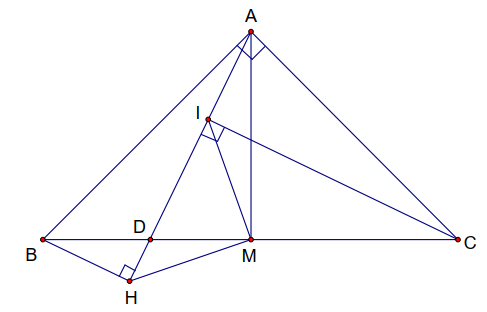
\includegraphics[width=0.5\textwidth]{25-4-lg.png}$$
        \begin{enumerate}[1.]
            \item \hfill
            \begin{enumerate}[a.]
                \item $*$ Chứng minh: $B A M=A C M$\\[5px]
                + Chứng minh được: $\triangle \mathrm{ABM}=\triangle \mathrm{ACM}(\mathrm{c}-\mathrm{c}-\mathrm{c})$\\[5px]
                + Lập luận được: $B A M=C A M=45^{\circ}$\\[5px]
                + Tính ra được $A C M=45^{\circ}$\\[5px]
                $\Rightarrow B A M=A C M$\\[5px]
                * Chứng minh: $\mathrm{BH}=\mathrm{AI}$.\\[5px]
                + Chỉ ra: $B A H=A C I$ (cùng phụ $D A C$ )\\[5px]
                + Chứng minh được $\triangle \mathrm{AIC}=\Delta \mathrm{BHA}$ (Cạnh huyên - góc nhọn)\\[5px]
                $\Rightarrow \mathrm{BH}=\mathrm{AI}$ (2 cạnh tương ứng)
                \item Tam giác MHI vuông cân.\\[5px]
                + Chứng minh được $A M \perp B C$\\[5px]
                + Chứng minh được $\mathrm{AM}=\mathrm{MC}$\\[5px]
                + Chứng minh được $H A M=I C M$\\[5px]
                + Chứng minh được $\Delta \mathrm{HAM}=\Delta \mathrm{ICM}(\mathrm{c}-\mathrm{g}-\mathrm{c})$\\[5px]
                $\Rightarrow \mathrm{HM}=\mathrm{MI}$(*)\\[5px]
                $\text {+ Do } \triangle \mathrm{HAM}=\triangle \mathrm{ICM} \Rightarrow H M A=I M C \Rightarrow H M B=I M A \text { (do } A M B=A M C=90^{\circ} \\[5px]
                \text {+ Lập luận được: } H M I=90^{\circ} \\[5px]
                \qquad \text {Từ }\left(^*\right) \text { và }\left({ }^{* *}\right)=>\Delta \mathrm{MHI} \text { vuông cân }$(**)\\[5px]
                Từ $\left({ }^*\right)$ và $\left({ }^{* *}\right)=>\Delta \mathrm{MHI}$ vuông cân
            \end{enumerate}
            \item \hfill 
            $$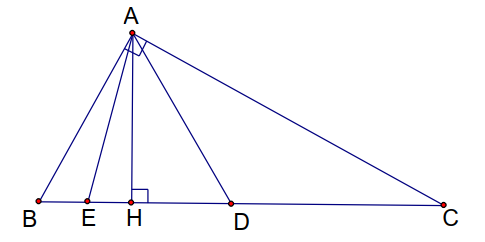
\includegraphics[width=0.5\textwidth]{25-4.2-lg.png}$$
            + Chứng minh được :\\[5px]
            $A E \mathrm{C}=A B C+B A E=H A D+D A C+B A E=E A H+H A D+D A C=E A C$\\[5px]
            (Vì $B$ và $H A C$ cùng phụ với $B A H$ )\\[5px]
            Suy ra tam giác $\mathrm{AEC}$ cân tại $\mathrm{C} \Rightarrow \mathrm{AC}=\mathrm{CE}$ (*)\\[5px]
            + Tương tự chứng minh được $\mathrm{AB}=\mathrm{BD}$
            $\left({ }^{* *}\right)$\\[5px]
            $+ \text { Từ }\left({ }^*\right) \text { và }\left({ }^{* *}\right) \Rightarrow \mathrm{AB}+\mathrm{AC}=\mathrm{BD}+\mathrm{EC}=\mathrm{ED}+\mathrm{BC}$
        \end{enumerate}
    }
\end{bt}

\begin{bt}
    Cho $\mathrm{x}, \mathrm{y}, \mathrm{z}$ là 3 số thực tùy ý thỏa mãn $\mathrm{x}+\mathrm{y}+\mathrm{z}=0$ và $-1 \leq x \leq 1$, $-1 \leq y \leq 1,$
    
    $-1 \leq z \leq 1$. Chứng minh rằng đa thức $x^2+y^4+z^6$ có giá trị không lớn hơn 2 .
\loigiai{
    +) Trong ba số $x, y, z$ có ít nhất hai số cùng dấu. Giả sử $x ; y \geq 0$\\[5px]
    $\Rightarrow \mathrm{z}=-\mathrm{x}-\mathrm{y} \leq 0 \\[5px]
    + \text { Vi }-1 \leq x \leq 1,-1 \leq y \leq 1,-1 \leq z \leq 1=>x^2+y^4+z^6 \leq|x|+|y|+|z| \\[5px]
    \Rightarrow x^2+y^4+z^6 \leq x+y-z \\[5px]
    \Rightarrow x^2+y^4+z^6 \leq-2 z \\[5px]
    +)-1 \leq z \leq 1 \text { và } \mathrm{z} \leq 0 \Rightarrow x^2+y^4+z^6 \leq 2 \\[5px]
    \text {KL: Vậy } x^2+y^4+z^6 \leq 2$
}
\end{bt}



	\onehalfspacing
\section{Đề số 26}

\begin{bt} 
   \begin{enumerate}[1)]
    \item Thực hiện phép tính
    \begin{enumerate}[a.]
        \item $\mathrm{A}=\frac{5}{15}+\frac{14}{25}-\frac{12}{9}+\frac{2}{7}+\frac{11}{25}$
        \item $B=\frac{2^{12} \cdot 3^5-4^6 \cdot 9^2}{\left(2^2 \cdot 3\right)^6+8^4 \cdot 3^5}-\frac{5^{10} \cdot 7^3-25^5 \cdot 49^2}{(125 \cdot 7)^3+5^9 \cdot 14^3}$
    \end{enumerate}
    \item Tìm $x, y, z$ biết:
    \begin{enumerate}[a.]
        \item $\left(3-\frac{9}{10}-|x+2|\right):\left(\frac{19}{10}-1-\frac{2}{5}\right)+\frac{4}{5}=1$ 
        \item $\frac{x}{3}=\frac{y}{4}, \frac{y}{3}=\frac{z}{5}$ và $2 x-3 y+z=6$
    \end{enumerate}
   \end{enumerate}
\loigiai{}
\end{bt}

\begin{bt}
    \hfill
	\begin{enumerate}[a.]
        \item Tìm x, y nguyên thoả mãn $3 x y-5=x^2+2 y$
        \item Chứng minh rằng với mọi số nguyên dương $\mathrm{n}$ thì: $3^{n+2}-2^{n+2}+3^n-2^n$ chia hết cho 10
    \end{enumerate}
	\loigiai{} 
\end{bt}

\begin{bt}
    Cho đa thức: $\mathrm{A}(\mathrm{x})=\mathrm{x}+\mathrm{x}^2+\mathrm{x}^3+\ldots+\mathrm{x}^{99}+\mathrm{x}^{100}$.
    \begin{enumerate}[a.]
        \item Chứng minh rằng $x=-1$ là nghiệm của $\mathrm{A}(\mathrm{x})$
        \item Tính giá trị biểu thức $\mathrm{A}(\mathrm{x})$ khi $\mathrm{x}=\frac{1}{2}$
    \end{enumerate}
	\loigiai{}
\end{bt}

\begin{bt}
    Cho $\triangle A B C(\mathrm{AB}>\mathrm{AC}), \mathrm{M}$ là trung điểm của $\mathrm{BC}$. Đường thẳng đi qua $\mathrm{M}$ vuông góc với tia phân giác của góc $B A C$ cắt cạnh $\mathrm{AB}, \mathrm{AC}$ lần lượt tại $\mathrm{E}$ và $\mathrm{F}$ (giao điểm của đường thẳng đó với tia phân giác góc $BAC$ là $H$ ). Chứng minh rằng:
    \begin{enumerate}[a.]
        \item $\mathrm{EH}=\mathrm{HF}$
        \item $2 \mathrm{BME}=\mathrm{ACB}-\mathrm{B}$.
        \item $\frac{F E^2}{4}+A H^2=A E^2$.
        \item $\mathrm{BE}=\mathrm{CF}$
    \end{enumerate}
	\loigiai{}
\end{bt}

\begin{bt}
   Giải bằng máy tính cầm tay:
   \begin{enumerate}[a.]
    \item Tính giá trị của đa thức $\mathrm{P}(\mathrm{x})=1+\mathrm{x}+\mathrm{x}^2+\mathrm{x}^3+\ldots .+\mathrm{x}^{10}$ tại $\mathrm{x}=2,13$ (kết quả ghi dưới dạng số thập phân lấy trên màn hình).
    \item Tìm 2 chữ số cuối của: $A=2^{2010}+2^{2011}+2^{2012}+2^{2013}+2^{2014}+2^{2015}+2^{2016}$
   \end{enumerate}
\loigiai{}
\end{bt}



	\onehalfspacing
\section{Đề số 27}

\begin{bt} 
   \hfill
   \begin{enumerate}[a.]
    \item Thực hiện phép tính: $A=\frac{2^{12} \cdot 3^5-4^6 \cdot 9^2}{\left(2^2 \cdot 3\right)^6+8^4 \cdot 3^5}$
    \item Cho hàm số $y=f(x)=a x^2+b x+c$.
    
    Cho biết $f(0)=2014 ; f(1)=2015 ; f(-1)=2017$. Tính $f(-2)$.
   \end{enumerate}
\loigiai{
    \begin{enumerate}
        \item $A=\frac{2^{12} \cdot 3^5-4^6 \cdot 9^2}{\left(2^2 \cdot 3\right)^6+8^4 \cdot 3^5}=\frac{2^{12} \cdot 3^5-2^{12} \cdot 3^4}{2^{12} \cdot 3^6+2^{12} \cdot 3^5} \\[5px]
        =\frac{2^{12} \cdot 3^4(3-1)}{2^{12} \cdot 3^5(3+1)}=\frac{2}{3 \cdot 4}=\frac{1}{6}$
        \item Ta có $f(0)=2014 \Leftrightarrow c=2014$
        $f(1)=2015 \Leftrightarrow a+b+c=2015 \Rightarrow a+b=1$ (1)\\[5px]
        $f(-1)=2017 \Leftrightarrow a-b+c=2017 \Rightarrow a-b=3$ (2)\\[5px]
        Từ (1)(2) suy ra: $a=2 ; b=-1$. Khi đó $f(x)=2 x^2-x+2014$\\[5px]
        Suy ra $f(-2)=2 \cdot(-2)^2-(-2)+2014=2024$
    \end{enumerate}
}
\end{bt}

\begin{bt}
   Tìm $x$, $y$ biết:
	\begin{enumerate}[a.]
        \item $\left|x+\frac{1}{5}\right|-4=-2$
        \item $2^{x-1}+5.2^{x-2}=\frac{7}{32}$
        \item $|x+5|+(3 y-4)^{2016}=0$
        \item $\frac{x}{2}=\frac{y}{5}$ và $x y=40$
    \end{enumerate}
	\loigiai{
        \begin{enumerate}
            \item $\left|x+\frac{1}{5}\right|-4=-2\\[5px] \Leftrightarrow\left|x+\frac{1}{5}\right|=2\\[5px] \Leftrightarrow\left[\begin{array}{l}x+\frac{1}{5}=2 \\[5px] x+\frac{1}{5}=-2\end{array} \Rightarrow\left[\begin{array}{l}x=\frac{9}{5} \\[5px] x=-\frac{11}{5}\end{array}\right.\right.$\\[5px]
            Vậy $x=\frac{9}{5} ; x=-\frac{11}{5}$
            \item $2^{x-1}+5 \cdot 2^{x-2}=\frac{7}{32}\\[5px] \Leftrightarrow 2^{x-1}\left(1+\frac{5}{2}\right)=\frac{7}{32} \Leftrightarrow 2^{x-1} \cdot \frac{7}{2}=\frac{7}{32} \Leftrightarrow 2^{x-1}=\frac{7}{32} \cdot \frac{2}{7}=\frac{1}{16}=2^{-4}$\\[5px]
            Suy ra $x-1=-4 \Leftrightarrow x=-3$. Vậy $x=-3$.
            \item $|x+5|+(3 y-4)^{2016}=0$. Vi $|x+5| \geq 0 ;(3 y-4)^{2016} \geq 0$\\[5px]
            Suy ra: $\left\{\begin{array}{l}|x+5|=0 \\[5px] (3 y-4)^{2016}=0\end{array} \Leftrightarrow\left\{\begin{array}{l}x+5=0 \\[5px] 3 y-4=0\end{array} \Leftrightarrow\left\{\begin{array}{l}x=-5 \\[5px] y=\frac{4}{3}\end{array}\right.\right.\right.$.\\[5px]
            Vậy $x=-5 ; y=\frac{4}{3}$
            \item Ta có: $\frac{x}{2}=\frac{y}{5}\\[5px] \Leftrightarrow \frac{x y}{2.5}=\frac{y^2}{5^2}\\[5px] \Leftrightarrow \frac{40}{10}=\frac{y^2}{25}\\[5px] \Rightarrow y^2=10^2 \Leftrightarrow y= \pm 10 \Rightarrow x= \pm 4$\\[5px]
            Vậy $(x ; y) \in\{(4 ; 10) ;(-4 ;-10)\}$
        \end{enumerate}
    } 
\end{bt}

\begin{bt}
    \hfill
    \begin{enumerate}[a.]
        \item Tìm tất cả các cặp số nguyên $x$, $y$ sao cho: $2 x y+x-2 y=4$
        \item Số $\mathrm{M}$ được chia thành ba số tỉ lệ với 0,$5 ; 1 \frac{2}{3} ; 2 \frac{1}{4}$. Tìm số $\mathrm{M}$ biết rằng tổng bình phương của ba số đó bằng 4660 .
    \end{enumerate}
	\loigiai{
        \begin{enumerate}
            \item $\text { 1) Ta có: } 2 x y+x-2 y=4 \Leftrightarrow x(2 y+1)-(2 y+1)=3 \Leftrightarrow(x-1)(2 y+1)=3 \\[5px]
            \Leftrightarrow(x-1)(2 y+1)=3=( \pm 1) \cdot( \pm 3)=( \pm 3) \cdot( \pm 1)$\\[5px] 
            $\begin{array}{|c|c|c|c|c|}
                \hline x-1 & 1 & -1 & 3 & -3 \\[5px]
                \hline x & 2 & 0 & 4 & -2 \\[5px]
                \hline 2 \mathrm{y}+1 & 3 & -3 & 1 & -1 \\[5px]
                \hline \mathrm{y} & 1 & -2 & 0 & -1 \\[5px]
                \hline
                \end{array}$\\[5px] 
            Vậy $(x ; y) \in\{(2 ; 1) ;(0 ;-2) ;(4 ; 0) ;(-2 ;-1)\}$
            \item Ta có $0,5: 1 \frac{2}{3}: 2 \frac{1}{4}=\frac{1}{2}: \frac{5}{3}: \frac{9}{4}=\frac{6}{12}: \frac{20}{12}: \frac{27}{12}=6: 20: 27$\\[5px]
            Giả sử $\mathrm{M}$ được chia thành 3 số là $x ; y ; z$.\\[5px] 
            Theo bài ra ta có:\\[5px]
            $\frac{x}{6}=\frac{y}{20}=\frac{z}{27} \Leftrightarrow \frac{x^2}{6^2}=\frac{y^2}{20^2}=\frac{z^2}{27^2}=\frac{x^2+y^2+z^2}{6^2+20^2+27^2}=\frac{4660}{1165}=4=2^2 \\[5px]           
            \Rightarrow x^2=12^2 \Rightarrow x= \pm 12 ; y^2=40^2 \Rightarrow y= \pm 40 ; z^2=54^2 \Rightarrow z= \pm 54 \\[5px]         
            \text {Vậy } M=12+40+54=106 \text { Hoặc } M=-12-40-54=-106$
        \end{enumerate}
    }
\end{bt}

\begin{bt}
    Cho tam giác $\mathrm{ABC}$ cân tại $\mathrm{A}$. Trên cạnh $\mathrm{BC}$ lấy điểm $\mathrm{D}$, trên tia đối của tia $C B$ lấy điểm $E$ sao cho $C E=B D$. Đường thẳng vuông góc với $B C$ kẻ từ $\mathrm{D}$ cắt $A B$ tại $M$. Đường vuông góc với $\mathrm{BE}$ tại $\mathrm{E}$ cắt $\mathrm{AC}$ tại $\mathrm{N}$.
    \begin{enumerate}[a.]
        \item Chứng minh: $\triangle M B D=\triangle N C E$.
        \item Cạnh $\mathrm{BC}$ cắt $\mathrm{MN}$ tại $\mathrm{I}$. Chứng minh $\mathrm{I}$ trung điểm của $\mathrm{MN}$.
        \item Chứng minh đường thẳng vuông góc với $\mathrm{MN}$ tại $\mathrm{I}$ luôn đi qua một điểm cố định khi D thay đổi trên đoạn BC.
    \end{enumerate}
	\loigiai{
        $$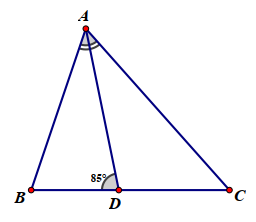
\includegraphics[width=0.4\textwidth]{13-4-lg.png}$$
        \begin{enumerate}
            \item Ta có $A B C=N C E=(A C B)$\\[5px]
            $\Rightarrow \triangle M B D=\triangle N C E(c g v-g n) \text {. }$
            \item Theo câu a)\\[5px]
            $\Rightarrow M D=E N \Rightarrow \triangle I M D=I N E(c g v-g n) \Rightarrow I M=I N \Rightarrow I \text { trung điểm } \mathrm{MN} \text {. }$\\[5px]
            \item $\text {Kẻ } A H \perp B C \\[5px]
            \Rightarrow \triangle A B H=\triangle A C H(c h-g n) \\[5px]
            \Rightarrow B A H=C A H$\\[5px]
            Đường vuông góc với $\mathrm{MN}$ tại $\mathrm{I}$ cắt $\mathrm{AH}$ tại $\mathrm{O}$.\\[5px]
            $\Rightarrow \triangle O A B=\triangle O A C(\text { c.g.c) } \\[5px]
            \Rightarrow O B A=O C A\\[5px]$
            Mặt khác :\\[5px]
            $\triangle O B H=\triangle O C H(2 c g v) \Rightarrow O B=O C (*)\\[5px] 
            \triangle O M I=\triangle O N I(2 c g v) \Rightarrow O M=O N (**)\\[5px]
            B M=C N \text { (câu b) }\left(^{* * *}\right)\\[5px]$
            Từ $\left({ }^*\right)\left({ }^{* *}\right)\left({ }^{* *}\right)$ suy ra :\\[5px]
            $\triangle O B M=\triangle O C N(\text { c.c.c }) \Rightarrow O B M=O C N$
            Từ (2)(3) $\Rightarrow O C A=O C N(=O B A)=90^{\circ} \Rightarrow O C \perp A C$\\[5px] 
            Vì $\mathrm{AC}$ cố định mà $O C \perp A C \Rightarrow \mathrm{O}$ cố định.\\[5px]
            $\text { Vậy đường thẳng vuông góc với } \mathrm{MN} \text { tại } \mathrm{I} \text { luôn đi qua điểm } \mathrm{O} \text { cố định. }$
        \end{enumerate}
    }
\end{bt}

\begin{bt}
   \hfill
   \begin{enumerate}[a.]
    \item Tìm số tự nhiên có ba chữ số. Biết rằng số đó chia hết cho 7 và tổng các chữ số đó bằng 14.
    \item Cho tam giác $\mathrm{ABC}$ có $B A C=B C A=80^{\circ}$. Ở miền trong của tam giác vẽ hai tia $\mathrm{Ax}$ và $C y$ cắt $\mathrm{BC}$ và $\mathrm{BA}$ lân lượt tại $\mathrm{D}$ và $\mathrm{E}$. Cho biết $C A D=60^{\circ} ; E C A=50^{\circ}$.
    Tính số đo góc $A D E$.
   \end{enumerate}
\loigiai{
    \begin{enumerate}
        \item Ta có:\\[5px]
        $\overline{a b c}: 7 \Leftrightarrow(100 a+10 b+c) \vdots 7 \Leftrightarrow(98 a+7 b+2 a+3 b+c) \vdots 7 \Leftrightarrow(2 a+3 b+c) \vdots 7(1)$\\[5px]
        Mặt khác theo bài ra :\\[5px]
        $a+b+c=14 \Rightarrow(a+b+c) \vdots 7 \Rightarrow(2 a+2 b+2 c) \vdots 7$\\[5px]
        Từ (1), (2) $\Rightarrow b-c \vdots 7 \Rightarrow b-c \in\{-7 ; 0 ; 7\}$\\[5px]
        +) Nếu $b-c=7$ có:\\[5px]
        $c=0 \Rightarrow b=7 \Rightarrow a=7 \\[5px]
        c=1 \Rightarrow b=8 \Rightarrow a=5$\\[5px] 
        $c=2 \Rightarrow b=9 \Rightarrow a=3$\\[5px]
        +) Nếu $b-c=0$ có:\\[5px]
        $b=c=6 \Rightarrow a=2 \\[5px]
        b=c=5 \Rightarrow a=4 \\[5px]
        b=c=4 \Rightarrow a=6 \\[5px]
        b=c=3 \Rightarrow a=8\\[5px]$
        +) Nếu $b-c=-7$ có:\\[5px]
        $c=b+7 \Rightarrow b =0 \Rightarrow c=7 \Rightarrow a=7 \\[5px]
        b=1 \Rightarrow c=8 \Rightarrow a=5 \\[5px]
        b=2 \Rightarrow c=9 \Rightarrow a=3\\[5px]$\\[5px]
        Vậy có 10 số thỏa mãn : 770; 581; 392; 266; 455; 644; 833; 707; 518; 329.
        \item 
        $$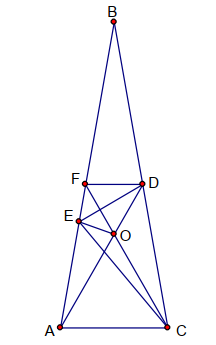
\includegraphics[width=0.35\textwidth]{27-5-lg.png}$$        
        Kẻ tia CF sao cho $A C F=60^{\circ}(F \in A B)$,
        Tia $\mathrm{CF}$ cắt $\mathrm{AD}$ tại $\mathrm{O}$.\\[5px]
        $\Rightarrow \triangle A O C ; \triangle F O D$ đều\\[5px] $\Rightarrow O A=O C=A C ; O F=O D=F D$.\\[5px]
        $\triangle A E C$ có $E A C=80^{\circ}, A C E=50^{\circ} \Rightarrow C E A=50^{\circ}$\\[5px]
        $\Rightarrow \triangle A C E$ cân tại $\mathrm{A}\\[5px] \Rightarrow A C=A E \Rightarrow \triangle A E O$ cân tại $\mathrm{A}$. Có:\\[5px]
        $E A O=20^{\circ} \Rightarrow A E O=A O E=80^{\circ} \Rightarrow E O F=40^{\circ}$\\[5px]
        Suy ra: $A F C=180^{\circ}-80^{\circ}-60^{\circ}=40^{\circ}=E O F$\\[5px]
        $\Rightarrow \triangle E O F$ cân tại $\mathrm{E} \Rightarrow E O=E F$\\[5px]
        $\Rightarrow \triangle F D E=\triangle O D E($ c.c.c)\\[5px]
        $\Rightarrow O D E=F D E=\frac{1}{2} F D A=\frac{1}{2} \cdot 60^{\circ}=30^{\circ}$ Vậy $A D E=30^{\circ}$.
    \end{enumerate}
}
\end{bt}



	\section{Đề số 28}

\begin{bt} 
   \hfill
   \begin{enumerate}[a.]
    \item Thực hiện phép tính: $\quad B=\frac{1}{-77^2} \cdot 7^4(-11)^2 \cdot 77^5 \cdot\left(\frac{1}{7^2}\right)^2:\left(7^3 \cdot 11^6\right)$
    \item Cho các số $a, b, c$ khác 0 thỏa mãn: $\frac{a-b+c}{2 b}=\frac{c-a+b}{2 a}=\frac{a-c+b}{2 c}$
    
    Tính giá trị biểu thức: $\mathrm{P}=\left(1+\frac{\mathrm{c}}{\mathrm{b}}\right) \cdot\left(1+\frac{\mathrm{b}}{\mathrm{a}}\right) \cdot\left(1+\frac{\mathrm{a}}{\mathrm{c}}\right)$
   \end{enumerate}
\loigiai{}
\end{bt}

\begin{bt}
    \hfill
	\begin{enumerate}[a.]
        \item Tìm $x$ biết: $\frac{2}{|x-2|+2}=\frac{3}{|6-3 x|+1}$
        \item Tìm hình chữ nhật có kích thước các cạnh là số nguyên sao cho số đo diện tích bằng số đo chu vi.
        \item Tìm các số nguyên dương x; y; z thỏa mãn:
        $$
        (x-y)^3+(y-z)^2+2015 \cdot|x-z|=2017
        $$
    \end{enumerate}
	\loigiai{} 
\end{bt}

\begin{bt}
    Cho hàm số: $\mathrm{y}=\mathrm{f}(\mathrm{x})=\mathrm{x}+\frac{3}{2}|\mathrm{x}|(1)$
    \begin{enumerate}[a.]
        \item Vẽ đồ thị hàm số (1).
        \item Gọi $E$ và $F$ là hai điểm thuộc đồ thị hàm số (1) có hoành độ lần lượt là (-4) và $\frac{4}{5}$, xác định tọa độ hai điểm $\mathrm{E}, \mathrm{F}$. Tìm trên trục tung điểm $\mathrm{M}$ để $EM+MF$ nhỏ nhất.
    \end{enumerate}
	\loigiai{}
\end{bt}

\begin{bt}
    \hfill
    \begin{enumerate}[1.]
        \item Cho tam giác $A B C$ nhọn; vẽ về phía ngoài tam giác $A B C$ các tam giác vuông cân tại $\mathrm{A}$ là tam giác $\mathrm{ABD}$ và tam giác $\mathrm{ACE}$.
        \begin{enumerate}[a.]
            \item Chứng minh $\mathrm{DC}=\mathrm{BE}$ và $\mathrm{DC} \perp \mathrm{BE}$.
            \item Gọi $\mathrm{H}$ là chân đường vuông góc kẻ từ $\mathrm{A}$ đến $\mathrm{ED}$ và $\mathrm{M}$ là trung điểm của đoạn thẳng $\mathrm{BC}$. Chứng minh $\mathrm{A}, \mathrm{M}, \mathrm{H}$ thẳng hàng .
        \end{enumerate}
        \item Cho tam giác $\mathrm{ABC}$ vuông tại $\mathrm{A}$ có $\mathrm{AB}=3 \mathrm{~cm} ; \mathrm{AC}=4 \mathrm{~cm}$. Điểm $I$ nằm trong tam giác và cách đều ba cạnh của tam giác $\mathrm{ABC}$. Gọi $\mathrm{M}$ là chân đường vuông góc kẻ từ điểm $I$ đến $BC$. Tính $MB$.
    \end{enumerate}
	\loigiai{}
\end{bt}

\begin{bt}
    Chứng minh rằng với mọi số tự nhiên $\mathrm{n} \geq 2$ thì tổng:
    $$
    \mathrm{S}=\frac{3}{4}+\frac{8}{9}+\frac{15}{16}+\ldots+\frac{\mathrm{n}^2-1}{\mathrm{n}^2} \text { không thể là một số nguyên. }
    $$
\loigiai{}
\end{bt}



	\onehalfspacing
\section{Đề số 29}

\begin{bt} 
   \hfill
   \begin{enumerate}[a.]
    \item  Tìm $x$, biết $|x-1|=\frac{2}{3}$;
    \item Tính giá trị của biểu thức sau: $\mathrm{A}=\frac{2 \mathrm{x}^2+3 x-1}{3 x-2}$ với $|x-1|=\frac{2}{3}$
   \end{enumerate}
\loigiai{
    \begin{enumerate}
        \item Ta có $|x-1|=\frac{2}{3} \Leftrightarrow\left[\begin{array}{c}x-1=\frac{2}{3} \\[5px] x-1=-\frac{2}{3}\end{array} \Leftrightarrow\left[\begin{array}{l}x=\frac{5}{3} \\[5px] x=\frac{1}{3}\end{array}\right.\right.$
        \item Từ câu 1):\\[5px] 
        Với $\mathrm{x}=\frac{5}{3}$ thay vào $\mathrm{A}$ ta được $\mathrm{A}=\frac{14}{27}$\\[5px] 
        Với $x=\frac{1}{3}$ thay vào $\mathrm{A}$ ta được $\mathrm{A}=-\frac{2}{9}$
    \end{enumerate}
}
\end{bt}

\begin{bt}
    \hfill
	\begin{enumerate}[a.]
        \item Tìm chữ số tận cùng của $A$ biết $A=3^{n+2}-2^{n+2}+3^n-2^n$
        \item Tìm các giá trị nguyên của $x$ để $\frac{x+3}{x-2}$ nhận giá trị nguyên.
    \end{enumerate}
	\loigiai{
        \begin{enumerate}
            \item Ta có:\\[5px]
            $A =3^{n+2}-2^{n+2}+3^n-2^n=3^n\left(3^2+1\right)-2^n\left(2^2+1\right)=10.3^n-2^n\left(2^2+1\right)=10.3^n-5.2^n \\[5px]
            =10.3^n-10.2^{n-1}=10\left(3^n-2^{n-1}\right) \vdots 10$\\[5px]
            A chia hết cho 10 suy ra chữ số tận cùng của $A$ là 0
            \item Ta có:\\[5px]
            $\frac{x+3}{x-2}=\frac{x-2+5}{x-2}=1+\frac{5}{x-2} \in Z \Leftrightarrow x-2 \in U(5)=\{ \pm 1 ; \pm 5\} \\[5px]
            \Rightarrow x=1 ; 3 ;-3 ; 7$
        \end{enumerate}
    } 
\end{bt}

\begin{bt}
    Cho đa thức $f(x)$ xác định với mọi $x$ thỏa mãn: $x \cdot f(x+2)=\left(x^2-9\right) \cdot f(x)$.
    \begin{enumerate}[a.]
        \item Tính $f(5)$.
        \item Chứng minh rằng $\mathrm{f}(\mathrm{x})$ có ít nhất 3 nghiệm.
    \end{enumerate}
	\loigiai{
        \begin{enumerate}
            \item Ta có với $x=3 \Rightarrow f(5)=0$
            \item $x=0 \Rightarrow f(0)=0 \Rightarrow x=0$ là một nghiệm\\[5px] 
            $x=3 \Rightarrow f(5)=0 \Rightarrow x=5$ là một nghiệm\\[5px] 
            $x=-3 \Rightarrow f(-1)=0 \Rightarrow x=-1$ là một nghiệm\\[5px] 
            Vậy $\mathrm{f}(\mathrm{x})$ có ít nhất là 3 nghiệm.
        \end{enumerate}
    }
\end{bt}

\begin{bt}
    Cho tam giác $\mathrm{ABC}$, trung tuyến $\mathrm{AM}$. Trên nửa mặt phẳng chứa đỉnh $\mathrm{C}$ bờ là đường thẳng $\mathrm{AB}$ dựng đoạn $\mathrm{AE}$ vuông góc với $\mathrm{AB}$ và $\mathrm{AE}=\mathrm{AB}$. Trên nửa mặt phẳng chứa đỉnh $\mathrm{B}$ bờ là đường thẳng $\mathrm{AC}$ dựng đoạn $\mathrm{AF}$ vuông góc với $\mathrm{AC}$ và $\mathrm{AF}=\mathrm{AC}$. Chứng minh rằng:
    \begin{enumerate}[a.]
        \item $F B=E C$
        \item $\mathrm{EF}=2 \mathrm{AM}$
        \item $\mathrm{AM} \perp \mathrm{EF}$.
    \end{enumerate}
	\loigiai{
        $$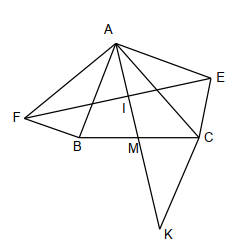
\includegraphics[width=0.45\textwidth]{29-4-lg.png}$$
        \begin{enumerate}
            \item Chứng minh $\triangle A B F=\triangle A E C(\operatorname{cgc}) \Rightarrow F B=E C$
            \item Trên tia đối của tia MA lấy $\mathrm{K}$ sao cho $\mathrm{AK}=2 \mathrm{AM}$. Ta có:\\[5px]
            $\triangle \mathrm{ABM}=\Delta \mathrm{KCM} \Rightarrow \mathrm{CK} / / \mathrm{AB} \\[5px]
            \Rightarrow A C K+C A B=E A F+C A B=180^{\circ} \Rightarrow A C K=E A F \\[5px]
            \triangle \mathrm{EAF} \text { và } \triangle \mathrm{KCA} \text { có } \mathrm{AE}=\mathrm{AB}=\mathrm{CK} \text {; } \\[5px]
            \mathrm{AF}=\mathrm{AC}(\mathrm{gt}) ; A C K=E A F \\[5px]
            \Rightarrow \Delta \mathrm{EAF}=\Delta \mathrm{KCA}(\mathrm{cgc}) \Rightarrow \mathrm{EF}=\mathrm{AK}=2 \mathrm{AM} .$ \\[5px]
            \item Từ $\triangle \mathrm{EAF}=\Delta \mathrm{KCA} \Rightarrow C A K=A F E\\[5px] 
            \Rightarrow A F E+F A K=C A K+F A K=90^{\circ}$\\[5px] 
            $\Rightarrow A K \perp E F$
        \end{enumerate}
    }
\end{bt}

\begin{bt}
    Cho $a, b, c, d$ là các số dương. Tìm giá trị nhỏ nhất của biểu thức:
    $$
    A=|x-a|+|x-b|+|x-c|+|x-d|
    $$
\loigiai{
    Không mất tính tổng quát, giả sử $\mathrm{a} \leq \mathrm{b} \leq \mathrm{c} \leq \mathrm{d}$. Áp dụng BĐT $|a|+|b| \geq|a+b|$, dấu bằng xảy $\mathrm{ra} \Leftrightarrow \mathrm{ab} \geq 0$ ta có:\\[5px]
    $|x-a|+|x-d| \geq|x-a|+|d-x| \geq|x-a+d-x|=d-a \\[5px]
    |x-b|+|x-c| \geq|x-b|+|c-x| \geq|x-b+c-x|=c-b$\\[5px]
    Suy ra $\mathrm{A} \geq \mathrm{c}+\mathrm{d}-\mathrm{a}-\mathrm{b}$. Dấu "=" xảy ra khi và chỉ khi dấu "=" ở (1) và (2) xảy ra \\[5px] 
    $\Leftrightarrow(x-a)(d-x) \geq 0$ và $(x-b)(c-x) \geq 0 \Leftrightarrow \mathrm{a} \leq \mathrm{x} \leq \mathrm{d}$ và $\mathrm{b} \leq \mathrm{x} \leq \mathrm{c}$.\\[5px]
    Do đó $\min \mathrm{A}=\mathrm{c}+\mathrm{d}-\mathrm{a}-\mathrm{b} \Leftrightarrow \mathrm{b} \leq \mathrm{x} \leq \mathrm{c}$.
}
\end{bt}



	\onehalfspacing
\section{Đề số 30}

\begin{bt} 
    Thực hiện phép tính:
    $$
    \mathrm{A}=\left(1-\frac{1}{2}\right)\left(1-\frac{1}{3}\right)\left(1-\frac{1}{4}\right) ; \quad \mathrm{B}=(0,25)^2 \cdot\left(\frac{1}{3}\right)^{-2}\left(\frac{4}{3}\right)^2 \cdot\left(\frac{1}{4}\right)^{-1}
    $$
\loigiai{}
\end{bt}

\begin{bt}
    \hfill
	\begin{enumerate}[a.]
        \item Tìm x biết: $|2 x-6|-4 x=12$
        \item Tìm $x$ biết: $\left(\frac{1}{2}+\frac{1}{3}+\ldots+\frac{1}{2015}\right) \cdot x=\frac{2014}{1}+\frac{2013}{2}+\ldots+\frac{2}{2013}+\frac{1}{2014}$
        \item Chứng minh rằng: Nếu $\frac{a}{b}=\frac{c}{d}$ thì $\frac{4 a+5 b}{4 a-5 b}=\frac{4 c+5 d}{4 c-5 d}$
        (Với $a, b, c, d \neq 0 ; 4 a \neq \pm 5 b ; 4 c \neq \pm 5 d$ )
    \end{enumerate}
	\loigiai{} 
\end{bt}

\begin{bt}
    Một vật chuyển động trên các cạnh hình vuông. Trên hai cạnh đầu vật chuyên động với vận tốc $5 \mathrm{~cm} / \mathrm{s}$, trên cạnh thứ ba với vận tốc $4 \mathrm{~cm} / \mathrm{s}$, trên cạnh thứ tư với vận tốc $3 \mathrm{~cm} / \mathrm{s}$. Hỏi độ dài cạnh hình vuông biết rằng tổng thời gian vật chuyển động trên bốn cạnh là 59 giây.
	\loigiai{}
\end{bt}

\begin{bt}
    Cho tam giác $A B C$ cân tại $A$. Trên cạnh $B C$ lấy điêm $D$, trên tia đối của tia $C B$ lấy điểm $\mathrm{E}$ sao cho $\mathrm{BD}=\mathrm{CE}$. Các đường thẳng vuông góc với $\mathrm{BC}$ kẻ từ $\mathrm{D}$ và $\mathrm{E}$ cắt $\mathrm{AB}, \mathrm{AC}$ lần lượt ở $M$, $N$.
    \begin{enumerate}[a.]
        \item  Chứng minh rằng: $\mathrm{DM}=\mathrm{EN}$.
        \item $\mathrm{MN}$ cắt $\mathrm{BC}$ tại $\mathrm{I}$.Chứng minh $\mathrm{I}$ là trung điểm của $\mathrm{MN}$.
        \item Chứng minh rằng đường thẳng vuông góc với $\mathrm{MN}$ tại $I$ luôn đi qua một điểm cố định khi $D$ thay đổi trên cạnh $BC$.
    \end{enumerate}
	\loigiai{}
\end{bt}

\begin{bt}
    Cho $f(x)=a x^2+b x+c$ với $a, b, c$ là các số hữu tỉ. Chứng tỏa rằng: $f(-2) \cdot f(3) \leq 0$.

    Biết rằng $13 a+b+2 c=0$
\loigiai{}
\end{bt}



	\onehalfspacing
\section{Đề số 31}

\begin{bt} 
	\hfill
	\begin{enumerate}[a.]
		\item Tìm tập hợp các số nguyên $x$ thỏa mãn $\frac{1}{2}-\left(\frac{1}{3}+\frac{1}{4}\right)<x<\frac{1}{24}-\left(\frac{1}{8}-\frac{1}{3}\right)$.
		\item Tìm các số a, b, c thỏa mãn $\frac{a}{2}=\frac{b}{3} ; \frac{b}{5}=\frac{c}{4}$ và $a-b+c=-49$.
	\end{enumerate}
	\loigiai{} 
\end{bt}

\begin{bt}
	\hfill
	\begin{enumerate}[a.]
		\item Tìm giá trị của $\mathrm{m}$ để đa thức $g(x)=x^4+m^2 x^3+m x^2+m x-1$ có nghiệm là $-1$.
		\item Tìm tổng các hệ số của đa thức sau khi phá ngoặc và sắp xếp, biết: $f(x)=\left(3 x^2-12 x+8\right)^{2013} \cdot\left(x^3-2 x^2+3 x-3\right)^{2014}$.
		\item Chứng minh rằng với mọi số nguyên dương $\mathrm{n}$ thì phân số $\frac{12 n+1}{30 n+2}$ là phân số tối giản.
	\end{enumerate}
	\loigiai{} 
\end{bt}

\begin{bt}
	Một xe tải chạy từ thành phố A đến hải cảng B gồm ba chặng đường dài bằng nhau, 
	nhưng chất lượng mặt đường xấu tốt khác nhau nên vận tốc trên mỗi chặng lần lượt bằng 
	40; 24 và 60 (km/h). Biết tổng thời gian đi từ A đến B là 5 giờ, tính độ dài quãng đường 
	AB?
	\loigiai{} 
\end{bt}

\begin{bt}
	Cho tam giác $\mathrm{ABC}$ vuông tại $\mathrm{A}$, có $\mathrm{C}=30^{\circ}$, kẻ $A H \perp B C(H \in B C)$. Trên đoạn $\mathrm{HC}$ lấy điểm $\mathrm{D}$ sao cho $\mathrm{HD}=\mathrm{HB}$. Từ $\mathrm{C}$ kẻ $\mathrm{CE} \perp \mathrm{AD}$. Chứng minh rằng:
	\begin{enumerate}[a.]
		\item $\mathrm{BAD}=60^{\circ}$;
		\item $\mathrm{EH}$ song song với $\mathrm{AC}$.
	\end{enumerate}
	\loigiai{}
\end{bt}

\begin{bt}
	\hfill
	\begin{enumerate}[a.]
		\item Tính giá trị của biểu thức $\mathrm{A}=1.3+2.4+3.5+4.6+\ldots+48.50$.
		\item Cho $B=\frac{1}{2^2}+\frac{1}{3^2}+\frac{1}{4^2}+\cdots+\frac{1}{100^2}$. Chứng minh rằng: $\mathrm{B}<\frac{3}{4}$.
	\end{enumerate}
	\loigiai{}
\end{bt}

	\section{Đề số 32}

\begin{bt} 
	\hfill
	\begin{enumerate}[a.]
		\item Tính giá trị của biểu thức $\mathrm{A}=\left(\frac{-4}{7}+\frac{2}{5}\right): \frac{2}{3}+\left(\frac{-3}{7}+\frac{3}{5}\right): \frac{2}{3}$
		\item Tính giá trị của biểu thức $\mathrm{B}=2 \mathrm{x}^2-3 \mathrm{x}+1$ với $|x|=\frac{1}{2}$.
		\item Tìm 3 số $x, y, z$ biết rằng: $\frac{x}{3}=\frac{y}{7} ; \frac{y}{2}=\frac{z}{5}$ và $x+y+z=-110$.
	\end{enumerate}
	\loigiai{} 
\end{bt}

\begin{bt}
	\hfill
	\begin{enumerate}[a.]
		\item Tìm tập hợp các số nguyên $x$, biết rằng:
		$$
		4 \frac{5}{9}: 2 \frac{5}{18}-7<x<\left(3 \frac{1}{5}: 3,2+4,5.1 \frac{31}{45}\right):\left(-21 \frac{1}{2}\right)
		$$
		\item Cho $\frac{a}{c}=\frac{c}{b}$. Chứng minh rằng: $\frac{a^2+c^2}{b^2+c^2}=\frac{a}{b}$
		\item Tính giá trị của biểu thức: $C=2 x^5-5 y^3+2015$ tại $x, y$ thỏa mãn:
		$$	|x-1|+(y+2)^{20}=0 $$
	\end{enumerate}
	\loigiai{} 
\end{bt}

\begin{bt}
	\hfill 
	\begin{enumerate}[a.]
		\item Tìm số tự nhiên có ba chữ số, biết rằng số đó là bội của 18 và các chữ số của nó tỉ lệ theo 1: 2: 3.
		\item Tìm tất cả các số tự nhiên $a, b$ sao cho : $2^{\mathrm{a}}+37=|b-45|+\mathrm{b}-45$.
	\end{enumerate}
	\loigiai{} 
\end{bt}

\begin{bt}
	Cho tam giác $\mathrm{ABC}$ có ba góc nhọn $(\mathrm{AB}<\mathrm{AC})$. Vẽ về phía ngoài tam giác $A B C$ các tam giác đều $A B D$ và $A C E$. Gọi $I$ là giao của $C D$ và $B E, K$ là giao của $A B$ và $D C$.
	\begin{enumerate}[a.]
		\item Chứng minh rằng: $\triangle \mathrm{ADC}=\triangle \mathrm{ABE}$.
		\item Chứng minh rằng: góc $\mathrm{DIB}=60^{\circ}$.
		\item Gọi $\mathrm{M}$ và $\mathrm{N}$ lân lượt là trung điểm của $\mathrm{CD}$ và $\mathrm{BE}$. Chứng minh rằng $\triangle \mathrm{AMN}$ đều.
		\item Chứng minh rằng IA là phân giác của góc DIE.
	\end{enumerate}
	\loigiai{}
\end{bt}

\begin{bt}
	Cho 20 số nguyên khác $0: a_1, a_2, a_3, \ldots, a_{20} $ có các tính chất sau: 
	\begin{itemize}[*]
		\item $a_1$ là số dương.
		\item Tổng của ba số viết liền nhau bất kì là một số dương.
		\item Tổng của 20 số đó là số âm.
	\end{itemize}
	Chứng minh rằng : $a_{1} . a_{14}+ a_{14} . a_{12}<a_1 \cdot a_{12}$.
	\loigiai{}
\end{bt}

	\onehalfspacing
\section{Đề số 33}

\begin{bt} 
	\hfill
	\begin{enumerate}[a.]
		\item Tính giá trị $A=1000-\left\{(-5)^3 \cdot(-2)^3-11 \cdot\left[7^2-5 \cdot 2^3+8\left(11^2-121\right)\right]\right\}$
		\item Tìm $x$ biết $\left(3-\frac{9}{10}-|x+2|\right):\left(\frac{19}{10}-1-\frac{2}{5}\right)+\frac{4}{5}=1$
		\item Tìm $x$ thỏa mãn $|x-10|^{10}+|x-11|^{11}=1$
	\end{enumerate}
	\loigiai{} 
\end{bt}

\begin{bt}
	\hfill
	\begin{enumerate}[a.]
		\item Tìm hai số dương khác nhau $x$, $y$ biết rằng: Tổng, hiệu và tích của chúng lân lượt tỉ lệ nghịch với $35 ; 210$ và 12 .
		\item Cho a, b, c là các số thực khác 0 . Tìm các số thực $\mathrm{x}, \mathrm{y}, \mathrm{z}$ khác 0 thoả mãn:
		$$
		\frac{x y}{a y+b x}=\frac{y z}{b z+c y}=\frac{z x}{c x+a z}=\frac{x^2+y^2+z^2}{a^2+b^2+c^2}
		$$
	\end{enumerate}
	\loigiai{} 
\end{bt}

\begin{bt}
	\hfill 
	\begin{enumerate}[a.]
		\item Tìm $x$, y nguyên thoả mãn $3 x y-5=x^2+2 y$
		\item Tìm số có bốn chữ số $\overline{a b c d}$ thỏa mãn đồng thời hai điều kiện sau:
		\begin{enumerate}[i.]
			\item $\overline{a b}, \overline{a d}$ là hai số nguyên tố;
			\item $\overline{d b}+\mathrm{c}=\mathrm{b}^2+\mathrm{d}$.
		\end{enumerate}
	\end{enumerate}
	\loigiai{} 
\end{bt}

\begin{bt}
	Cho tam giác $A B C$ có $\hat{B}<90^{\circ}$ và $\hat{B}=2 \hat{C}$. Trên tia đối của tia $\mathrm{BA}$ lấy điểm $\mathrm{E}$ sao cho $\mathrm{BE}=\mathrm{BH}$ (với $\mathrm{H}$ là chân đường vuông góc kẻ từ $\mathrm{A}$ đến $\mathrm{BC}$ ), đường thẳng $\mathrm{EH}$ cắt $\mathrm{AC}$ ở $\mathrm{D}$.
	\begin{enumerate}[a.]
		\item Chứng minh rằng: $\mathrm{DA}=\mathrm{DC}$.
		\item Chứng minh rằng: $\mathrm{AE}=\mathrm{HC}$.
	\end{enumerate}
	\loigiai{}
\end{bt}

	\onehalfspacing
\section{Đề số 34}

\begin{bt} 
	\hfill
	\begin{enumerate}[a.]
		\item Chứng minh: $5^{2014}-5^{2013}+5^{2012}$ chia hết cho 105 .
		\item Tìm số nguyên tố $\mathrm{p}$ sao cho $\mathrm{p}+2$ và $\mathrm{p}+4$ đều là số nguyên tố.
	\end{enumerate}
	\loigiai{} 
\end{bt}

\begin{bt}
	Tìm x biết:
	\begin{enumerate}[a.]
		\item $|3-2 x|=x+1$
		\item $\left(\frac{1}{2}+\frac{1}{3}+\ldots+\frac{1}{2014}\right) \cdot x=\frac{2013}{1}+\frac{2012}{2}+\ldots+\frac{2}{2012}+\frac{1}{2013}$
	\end{enumerate}
	\loigiai{} 
\end{bt}

\begin{bt}
	\hfill 
	\begin{enumerate}[a.]
		\item Tìm $x ; y ; z$ biết $\frac{x}{y}=\frac{3}{2} ; 5 x=7 z$ và $x-2 y+z=32$.
		\item Cho $\frac{7 x+5 y}{3 x-7 y}=\frac{7 z+5 t}{3 z-7 t}$. Chứng minh: $\frac{x}{y}=\frac{z}{t}$.
		\item Tìm giá trị nhỏ nhất của $\mathrm{A}=|x-2013|+|2014-x|+|x-2015|$.
	\end{enumerate}
	\loigiai{} 
\end{bt}

\begin{bt}
	Cho tam giác $A B C$ cân $(A B=A C)$. Trên cạnh $B C$ lấy điểm $D$ trên tia đối tia $C B$ lấy điểm $E$ sao cho $\mathrm{BD}=\mathrm{CE}$. Các đường thẳng vuông góc với $\mathrm{BC}$ kẻ từ $\mathrm{D}$ và $\mathrm{E}$ cắt $\mathrm{AB}$ và $\mathrm{AC}$ lân lượt ở $\mathrm{M}$ và N. Gọi I là giao điểm của $\mathrm{MN}$ và $\mathrm{BE}$.
	\begin{enumerate}[a.]
		\item Biết $\mathrm{AB}<\mathrm{BC}$. Chứng minh: $\hat{\mathrm{A}}>60^{\circ}$.
		\item Chứng $\operatorname{minh} \mathrm{IM}=\mathrm{IN}$
		\item Chứng minh đường thẳng vuông góc với $\mathrm{MN}$ tại I luôn đi qua 1 điểm cố định khi $\mathrm{D}$ thay đối trên cạnh $B C$.
	\end{enumerate}
	\loigiai{}
\end{bt}
	\onehalfspacing
\section{Đề số 35}

\begin{bt} 
	\hfill
	\begin{enumerate}[1.]
		\item Tính giá trị của biểu thức
		$$
		\begin{aligned}
			& \mathrm{A}=(-1)^3 \cdot\left(-\frac{7}{8}\right)^3 \cdot\left(-\frac{2}{7}\right)^2 \cdot(-7) \cdot\left(-\frac{1}{14}\right) \\[5px]
			& \mathrm{B}=2016:\left(\frac{0,4-\frac{2}{9}+\frac{2}{11}}{1,4-\frac{7}{9}+\frac{7}{11}} \cdot \frac{-1 \frac{1}{6}+0,875-0,7}{\frac{1}{3}-0,25+\frac{1}{5}}\right)
		\end{aligned}
		$$
		\item Cho đa thức $Q(x)=a x^3+b x^2+c x+d$ với $a, b, c, d \in Z$. Biết $Q(x)$ chia hết cho 3 với mọi $x \in Z$. Chứng tỏ các hệ số $a, b, c, d$ đều chia hết cho 3.
	\end{enumerate}
	\loigiai{
		\begin{enumerate}
			\item $A=(-1) \cdot \frac{(-7)^3}{8^3} \cdot \frac{(-2)^2}{7^2} \cdot \frac{1}{2} \\[5px]
			= \frac{(-1) \cdot(-7)^3 \cdot(-2)^2}{2^9 \cdot 7^2 \cdot 2} \\[5px]
			= \frac{(-1) \cdot(-7) \cdot(-1)}{2^8} \\[5px]
			= \frac{-7}{256}$\\[5px]
			Tính:\\[5px]
			*) $ \frac{0,4-\frac{2}{9}+\frac{2}{11}}{1,4-\frac{7}{9}+\frac{7}{11}}=\frac{2 \cdot\left(\frac{1}{5}-\frac{1}{9}+\frac{1}{11}\right)}{7 \cdot\left(\frac{1}{5}-\frac{1}{9}+\frac{1}{11}\right)} \\[5px]
			= \frac{2}{7}\left(\text { vì } \frac{1}{5}-\frac{1}{9}+\frac{1}{11} \neq 0\right)$\\[5px] 
			*) $\frac{-1 \frac{1}{6}+0,875-0,7}{\frac{1}{3}-0,25+\frac{1}{5}}=\frac{-7 \cdot\left(\frac{1}{6}-\frac{1}{8}+\frac{1}{10}\right)}{2 \cdot\left(\frac{1}{6}-\frac{1}{8}+\frac{1}{10}\right)} \\[5px]
			=\frac{-7}{2}\left(\text { vì } \frac{1}{6}-\frac{1}{8}+\frac{1}{10} \neq 0\right) \\[5px]
			\text {B } = 2016:\left(\frac{2}{7} \cdot \frac{-7}{2}\right)=-2016$
			\item Cho đa thức $Q(x)=a x^3+b x^2+c x+d$\\[5px] $\text{Vì } \mathrm{Q}(\mathrm{x})$ : 3 với mọi $x \in Z$, nên\\[5px]
			$\text {Với } \mathrm{x}=0 \text {, ta có } \mathrm{Q}(0)=d \vdots 3 \\[5px]
			\text {Với } \mathrm{x}=1 \text {, ta có } \mathrm{Q}(1)=a+b+c+d \vdots 3 \\[5px]
			\text {mà } \mathrm{d} \vdots 3=>\mathrm{a}+\mathrm{b}+\mathrm{c} \vdots 3(1) \\[5px]
			\text {Với } \mathrm{x}=-1 \text {, ta có } \mathrm{Q}(-1)=-\mathrm{a}+\mathrm{b}-\mathrm{c}+\mathrm{d} \vdots 3 \\[5px]
			\text {mà } \mathrm{d} \vdots 3=>-\mathrm{a}+\mathrm{b}-\mathrm{c} \vdots 3(2) \\[5px]
			\mathrm{Q}(1)+\mathrm{Q}(-1)=2 \mathrm{~b} \vdots 3 \text { mà }(2 ; 3)=1 \text { nên } \mathrm{b} \vdots 3 \\[5px]
			\mathrm{Q}(1)-\mathrm{Q}(-1)=2(a+c) \vdots 3 \text { mà }(2 ; 3)=1 \text { nên } \mathrm{a}+\mathrm{c} \vdots 3(3) \\[5px]
			\text {Với } \mathrm{x}=2, \text { ta có } \mathrm{Q}(2)=8 \mathrm{a}+4 \mathrm{~b}+2 \mathrm{c}+\mathrm{d} \vdots 3 \\[5px]
			\text {hay } 7 \mathrm{a}+(\mathrm{a}+\mathrm{c})+2 \mathrm{~b}+\mathrm{d} \vdots 3 \\[5px]
			\text {Mà } \mathrm{d} \vdots 3, \mathrm{a}+\mathrm{c} \vdots 3, \mathrm{~b} \vdots 3 \text{ nên } 7 \mathrm{a} \vdots 3 \text { mà }(7 ; 3)=1=\mathrm{a} \vdots 3 \\[5px]
			\text {Từ (3) suy ra } \mathrm{c} \vdots 3=>\text{đpcm}$
		\end{enumerate}
	} 
\end{bt}

\begin{bt}
	\hfill
	\begin{enumerate}[1.]
		\item Biết $\frac{b z-c y}{a}=\frac{c x-a z}{b}=\frac{a y-b x}{c}($ với $a, b, c \neq 0)$.
		Chứng minh rằng: $\frac{\mathrm{x}}{\mathrm{a}}=\frac{\mathrm{y}}{\mathrm{b}}=\frac{\mathrm{z}}{\mathrm{c}}$.
		\item Số $\mathrm{M}$ được chia thành ba phân tỉ lệ nghịch với $3 ; 5 ; 6$. Biết rằng tổng các lập phương của ba phần đó là 10728 . Hãy tìm số $\mathrm{M}$.
	\end{enumerate}
	\loigiai{
		\begin{enumerate}
			\item Với a, b, c $\neq 0$, ta có:\\[5px]
			$\frac{b z-c y}{a}=\frac{c x-a z}{b}=\frac{a y-b x}{c}=\frac{b z a-c y a}{a^2}=\frac{b c x-b a z}{b^2}=\frac{a c y-b c x}{c^2} \\[5px]
			=\frac{b z a-c y a+b c x-b a z+a c y-b c x}{a^2+b^2+c^2}=\frac{0}{a^2+b^2+c^2}=0$\\[5px]
			Suy ra $\frac{\mathrm{bz}-\mathrm{cy}}{\mathrm{a}}=0$, do đó $\mathrm{bz}=\mathrm{cy} \Rightarrow \frac{\mathrm{y}}{\mathrm{b}}=\frac{\mathrm{z}}{\mathrm{c}}(1)$\\[5px]
			$\frac{\mathrm{cx}-\mathrm{az}}{\mathrm{b}}=0, \text { do đó } \mathrm{cx}=\mathrm{az} \Rightarrow \frac{\mathrm{x}}{\mathrm{a}}=\frac{\mathrm{z}}{\mathrm{c}}$ (2)\\[5px]
			Từ (1) và (2) suy ra $\frac{\mathrm{x}}{\mathrm{a}}=\frac{\mathrm{y}}{\mathrm{b}}=\frac{\mathrm{c}}{\mathrm{z}}$
			\item Gọi ba phần được chia của số $M$ là $x, y, z$. , ta được $x+y+z=M$\\[5px]
			Theo đề bài ta có $\mathrm{x}: \mathrm{y}: \mathrm{z}=\frac{1}{3}: \frac{1}{5}: \frac{1}{6}$ và $x^3+y^3+z^3=10728(1)$\\[5px]
			Hay $\frac{\mathrm{x}}{10}=\frac{\mathrm{y}}{6}=\frac{\mathrm{z}}{5}=k$ và $x^3+y^3+z^3=10728$\\[5px]
			Suy ra $x^3=10^3 \cdot k^3 ; y^3=6^3 \cdot k^3 ; z=5^3 \cdot k^3$\\[5px]
			Thay vào (1), được $1341 k^3=8 \Rightarrow k=2$
			suy ra $20 ; y=12 ; z=10 \quad$\\[5px] 
			Vậy $M=42$.
		\end{enumerate}
	} 
\end{bt}

\begin{bt}
	Cho tam giác $\mathrm{ABC}$ đều. Trên cạnh $\mathrm{AB}$ lấy điểm $\mathrm{D}$ sao cho $\mathrm{BD}=\frac{1}{3} \mathrm{AB}$. Tại $\mathrm{D}$ kẻ đường vuông góc với $\mathrm{AB}$ cắt cạnh $\mathrm{BC}$ tại $\mathrm{E}$. Tại $\mathrm{E}$ kẻ đường vuông góc với $\mathrm{BC}$ cắt $\mathrm{AC}$ tại $\mathrm{F}$.
	\begin{enumerate}[1.]
		\item Chứng minh $\mathrm{DF} \perp \mathrm{AC}$. Biết trong tam giác vuông cạnh đối diện với góc $30^{\circ}$ thì bằng nửa cạnh huyền.
		\item Chứng minh tam giác DEF đều.
		\item Gọi $G$ là trọng tâm của tam giác $D E F$. Chứng minh $G A=G B=G C$.
	\end{enumerate}
	\loigiai{
		$$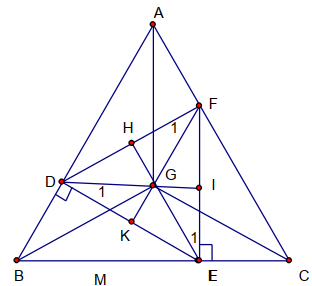
\includegraphics[width=0.45\textwidth]{35-3-lg.png}$$
		\begin{enumerate}
			\item $\triangle \mathrm{ABC}$ đều nên $\mathrm{AB}=\mathrm{AC}=\mathrm{BC}=\mathrm{a}$ và $\angle \mathrm{A}=\angle \mathrm{B}=\angle \mathrm{C}=60^{\circ}$\\[5px]
			$\mathrm{BD}=\frac{1}{3} \mathrm{a} \quad$ (gt)\\[5px] $\Rightarrow \mathrm{AD}=\frac{2}{3} \mathrm{a}$\\[5px]
			Xét $\triangle \mathrm{BDE}$ vuông tại $\mathrm{D}$ có $\angle \mathrm{B}=60^{\circ} \Rightarrow \angle \mathrm{DEB}=30^{\circ}$\\[5px]
			Xét $\triangle \mathrm{BDE}$ vuông tại $\mathrm{D}$ có $\angle \mathrm{DEB}=30^{\circ}\\[5px] 
			\Rightarrow \mathrm{BD}=\frac{1}{2} \mathrm{BE}$\\[5px]
			hay $\mathrm{BE}=2 \mathrm{BD}=2 \cdot \frac{1}{3} \mathrm{a}=\frac{2}{3} \mathrm{a}$ mà $\mathrm{BC}=\mathrm{a}$ nên $\mathrm{EC}=\frac{1}{3} \mathrm{a}$\\[5px]
			Tương tự, xét $\triangle \mathrm{ECF}$ vuông tại $\mathrm{E}$ có $\angle \mathrm{C}=60^{\circ}\\[5px] \Rightarrow \angle \mathrm{EFC}=30^{\circ}$\\[5px]
			$\Rightarrow \mathrm{AF}=\frac{1}{3} \mathrm{a}$\\[5px]
			Xét $\triangle \mathrm{ADF}$ và $\triangle \mathrm{BED}$ có:\\[5px]
			$\mathrm{AD}=\mathrm{BE}\left(=\frac{2}{3} \mathrm{a}\right)$\\[5px]
			$\angle \mathrm{A}=\angle \mathrm{B}\left(=60^{\circ}\right)$\\[5px]
			$\mathrm{AF}=\mathrm{BD}\left(=\frac{1}{3} \mathrm{a}\right)$\\[5px]
			$\Rightarrow \triangle \mathrm{ADF}=\triangle \mathrm{BED}($ c. g. c)\\[5px]
			$\Rightarrow \angle \mathrm{AFD}=\angle \mathrm{BDE}$ ( hai góc tương ứng)\\[5px]
			Mà $\angle \mathrm{BDE}=90^{\circ} \\[5px]
			\Rightarrow \angle \mathrm{AFD}=90^{\circ}$ hay $\mathrm{DF} \perp \mathrm{AC}$
			\item Chứng minh tương tự cũng có $. \Delta \mathrm{DBE}=\Delta \mathrm{ECF}$ (c.g.c)\\[5px] 
			$\Rightarrow \mathrm{DE}=\mathrm{EF}$ ( hai cạnh tương ứng)\\[5px] 
			Có $\triangle \mathrm{ADF}=\Delta \mathrm{BED}$ ( c. g. $\mathrm{c}$ ) $(\mathrm{cmt})\\[5px] 
			\Rightarrow \mathrm{DF}=\mathrm{DE}$ ( hai cạnh tương ứng)\\[5px] 
			$\Rightarrow \mathrm{DE}=\mathrm{DF}=\mathrm{EF}\\[5px] \Rightarrow \Delta \mathrm{DEF}$ là tam giác đều.
			\item Xét $\triangle D E F$ đều có $G$ là trọng tâm của tam giác\\[5px] 
			$\Rightarrow G$ là giao điểm của ba đường phân giác\\[5px] 
			$\Rightarrow \mathrm{GD}, \mathrm{GE}, \mathrm{GF}$ là các đường phân giác của các góc $\angle \mathrm{EDF} ; \angle \mathrm{DEF} ; \angle \mathrm{DFE}$ Có $\triangle \mathrm{DEF}$ đều nên $\angle \mathrm{D}=\angle \mathrm{E}=\angle \mathrm{F}=60^{\circ}$
		\end{enumerate}
	}
\end{bt}

\begin{bt}
	Cho tam giác $\mathrm{ABC}$, trung tuyến $\mathrm{AM}$ và $\mathrm{BE}$ cắt nhau tại $\mathrm{G}$. Chứng minh rằng nếu $\mathrm{AGB} \leq 90^{\circ}$ thì $\mathrm{AC}+\mathrm{BC}>3 \mathrm{AB}$.
	\loigiai{
		$$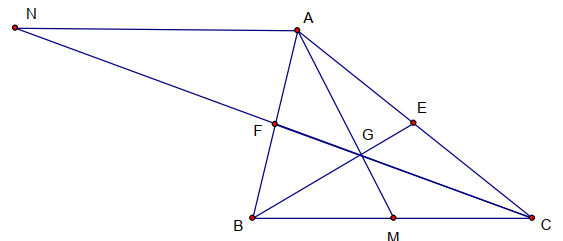
\includegraphics[width=0.65\textwidth]{35-4-lg.png}$$
		Vẽ trung tuyến CF của Tam giác $\mathrm{ABC}$. Trên tia đối của tia $F C$ lấy điểm $\mathrm{N}$ sao cho $\mathrm{FN}=\mathrm{FC}$.\\[5px]
		$\mathrm{C} / \mathrm{M}$ được $: \triangle \mathrm{ANF}=\Delta \mathrm{BCF}(\mathrm{c}-\mathrm{g}-\mathrm{c}) \Rightarrow \mathrm{AN}=\mathrm{BC}$\\[5px]
		Xét $\triangle \mathrm{CAN}$ có $\mathrm{AN}+\mathrm{AC}>\mathrm{NC}$ ( bất đẳng thức tam giác)\\[5px]
		$\Rightarrow \mathrm{AC}+\mathrm{BC}>\mathrm{NC}$\\[5px]
		Vì $\mathrm{G}$ là trọng tâm của tam giác $\mathrm{ABC}$ nên $\mathrm{CF}=3 \mathrm{GF} \Rightarrow \mathrm{NC}=6 \mathrm{GF}$ (1)\\[5px]
		Ta sẽ chứng minh: nếu $\angle \mathrm{AGB} \leq 90^{\circ}$ thì $\mathrm{GF} \geq \frac{A B}{2}$\\[5px]
		Giả sử $\mathrm{GF}<\frac{A B}{2}$ hay $\mathrm{GF}<\mathrm{AF}=\mathrm{BF}$ thì $\angle \mathrm{FAG}<\angle \mathrm{AGF} ; \angle \mathrm{FBG}<\angle \mathrm{BGF}$ ( quan hệ góc và cạnh tương ứng trong tam giác)\\[5px]
		$\Rightarrow \angle \mathrm{ABG}+\angle \mathrm{BAG}<\angle \mathrm{FGB}+\angle \mathrm{FGA}=\angle \mathrm{AGB} \leq 90^{\circ}$\\[5px]
		Xét tam giác $\mathrm{AGB}$ có $\angle \mathrm{ABG}+\angle \mathrm{BAG}+\angle \mathrm{AGB}<90^{\circ}+90^{\circ}=180^{\circ}$ vô lí.\\[5px]
		Vậy nếu $\angle \mathrm{AGB} \leq 90^{\circ}$ thì $\mathrm{GF} \geq \frac{A B}{2}$ (2)\\[5px] 
		$\text { Từ (1) và (2) } \Rightarrow N C \geq 3 A B \text { suy ra } \mathrm{AC}+\mathrm{BC}>3 \mathrm{AB} \text { (đpcm) }$
	} 
\end{bt}

\begin{bt}
	Tìm các giá trị nguyên của $x$ để biểu thức $C=\frac{22-3 x}{4-x}$ có giá trị lớn nhất.
	\loigiai{
		Biến đổi $C=\frac{22-3 x}{4-x}=\frac{3(4-x)+10}{4-x}=3+\frac{10}{4-x}$\\[5px]
		C có giá trị lớn nhất khi và chỉ khi $\frac{10}{4-x}$ có giá trị lớn nhất\\[5px]
		Có $x \in Z$, ta xét các trường hợp sau:\\[5px]
		Với $x>4 \Rightarrow 4-x<0$ thì $\frac{10}{4-x}<0$\\[5px]
		Với $x>4 \Rightarrow 4-x>0$.\\[5px] 
		Phân số $\frac{10}{4-x}$ có tử và mẫu đều dương, tử không đổi nên có giá trị lớn nhất khi mẫu nhỏ nhất\\[5px]
		Có $x \in Z$ Suy ra $4-x \in Z$\\[5px]
		Suy ra $4-x$ là số nguyên dương nhỏ nhất $\Rightarrow 4-x=1 \Rightarrow x=3$\\[5px]
		khi đó $\frac{10}{4-x}$ có giá trị là $10(2)$\\[5px]
		Từ (1) và (2) , phân số $\frac{10}{4-x}$ lớn nhất bằng 10\\[5px]
		Vậy GTLN của $C$ bằng 13 khi và chỉ khi $x=3$
	}
\end{bt}

	\section{Đề số 36}

\begin{bt} 
	\hfill
	\begin{enumerate}[a.]
		\item Cho a, b, c là ba số thực dương thỏa mãn điều kiện: $\frac{a+b-c}{c}=\frac{b+c-a}{a}=\frac{c+a-b}{b}$. \\Hãy tính giá trị của biểu thức: $B=\left(1+\frac{b}{a}\right)\left(1+\frac{a}{c}\right)\left(1+\frac{c}{b}\right)$.
		\item Cho tỉ lệ thức $\frac{a}{b}=\frac{c}{d}$ với $a \neq 0, b \neq 0, c \neq 0, d \neq 0, a \neq \pm b, c \neq \pm d$.
		\\Chứng minh: $\left(\frac{a-b}{c-d}\right)^{2013}=\frac{a^{2013}+b^{2013}}{c^{2013}+d^{2013}}$
	\end{enumerate}
	
	\loigiai{} 
\end{bt}

\begin{bt}
	\hfill
	\begin{enumerate}[a.]
		\item Cho $\frac{x}{y+z+t}=\frac{y}{z+t+x}=\frac{z}{t+x+y}=\frac{t}{x+y+z}$
		\\Chứng minh rằng: Biểu thức sau có giá trị nguyên
		$$
		A=\frac{x+y}{z+t}+\frac{y+z}{t+x}+\frac{z+t}{x+y}+\frac{t+x}{y+z}
		$$
		\item Tìm $x$ biết: $x^2-5 x+6=0$
		\item Số $\mathrm{A}$ được chia thành ba phần số tỉ lệ theo $\frac{2}{5}: \frac{3}{4}: \frac{1}{6}$. Biết rằng tổng các bình phương của ba số đó bằng 24309 . Tìm số $\mathrm{A}$.
	\end{enumerate}
	\loigiai{} 
\end{bt}

\begin{bt}
	Tìm giá trị nhỏ nhất của biểu thức: $A=|x-2013|+|x-3014|+|x-2015|$
	\loigiai{} 
\end{bt}

\begin{bt}
	Tìm hai số dương biết tổng, hiệu, tích của chúng tỉ lệ nghịch với ba số 20;120;16.
	\loigiai{}
\end{bt}

\begin{bt}
	Cho tam giác $\mathrm{ABC}$ vuông ở $\mathrm{A}$, có góc $C=30^{\circ}$, đường cao $\mathrm{AH}$. Trên đoạn $\mathrm{HC}$ lấy điểm $\mathrm{D}$ sao cho $H D=H B$. Từ $\mathrm{C}$ kẻ $\mathrm{CE}$ vuông góc với $\mathrm{AD}$. Chứng minh:
	\begin{enumerate}[a.]
		\item Tam giác $\mathrm{ABD}$ là tam giác đều.
		\item $A H=C E$.
		\item HE song song với $A C$.
	\end{enumerate}
	\loigiai{}
\end{bt}



	\onehalfspacing
\section{Đề số 37}

\begin{bt} 
	\hfill
	\begin{enumerate}[a.]
		\item Tính giá trị biểu thức $\mathrm{P}=\left|a-\frac{1}{2014}\right|+\left|a-\frac{1}{2016}\right|$, với $a=\frac{1}{2015}$.
		\item Tìm số nguyên $\mathrm{x}$ để tích hai phân số $\frac{6}{x+1}$ và $\frac{x-1}{3}$ là một số nguyên.
	\end{enumerate}
	\loigiai{} 
\end{bt}

\begin{bt}
	\hfill
	\begin{enumerate}[a.]
		\item Cho $\mathrm{a}>2, \mathrm{~b}>2$. Chứng minh $a b>a+b$
		\item Cho ba hình chữ nhật, biết diện tích của hình thứ nhất và diện tích của hình thứ hai tỉ lệ với 4 và 5 , diện tích hình thứ hai và diện tích hình thứ ba tỉ lệ với 7 và 8 , hình thứ nhất và hình thứ hai có cùng chiều dài và tổng các chiều rộng của chúng là $27 \mathrm{~cm}$, hình thứ hai và hình thứ ba có cùng chiều rộng, chiều dài của hình thứ ba là $24 \mathrm{~cm}$. Tính diện tích của mỗi hình chữ nhật đó.
	\end{enumerate}
	\loigiai{} 
\end{bt}

\begin{bt}
	Cho tam giác $A B C, M$ là trung điểm của $B C$. Trên tia đối của tia MA lấy điểm $E$ sao cho $\mathrm{ME}=\mathrm{MA}$. Chứng minh rằng:
	\begin{enumerate}[a.]
		\item AC = EB và AC // BE
		\item Gọi I là một điểm trên $\mathrm{AC}, \mathrm{K}$ là một điểm trên $\mathrm{EB}$ sao cho: $\mathrm{AI}=\mathrm{EK}$. Chứng minh: $\mathrm{I}, \mathrm{M}, \mathrm{K}$ thẳng hàng.
		\item Từ $\mathrm{E}$ kẻ $\mathrm{EH} \perp \mathrm{BC}(\mathrm{H} \in \mathrm{BC})$. Biết góc $\mathrm{HBE}$ bằng $50^{\circ}$; góc $\mathrm{MEB}$ bằng $25^{\circ}$, tính các góc $H E M$ và $B M E$ ?
	\end{enumerate}
	\loigiai{}
\end{bt}

\begin{bt}
	Cho các số $0<a_1<a_2<a_3<\ldots . .<a_{15}$. Chứng minh rằng $\frac{a_1+a_2+a_3+\ldots+a_{15}}{a_5+a_{10}+a_{15}}<5$
	\loigiai{}
\end{bt}

\begin{bt}
	Cho $\triangle \mathrm{ABC}$ nhọn với $B A C=60^{\circ}$. Chứng minh rằng:
	$$
	\mathrm{BC}^2=\mathrm{AB}^2+\mathrm{AC}^2-\mathrm{AB} \cdot \mathrm{AC}
	$$
	\loigiai{} 
\end{bt}
	\section{Đề số 38}

\begin{bt} 
	Tính các giá trị biểu thức sau:
	\\$A=\frac{\frac{1}{9}-\frac{1}{7}-\frac{1}{11}}{\frac{4}{9}-\frac{4}{7}-\frac{4}{11}}+\frac{0,6-\frac{3}{25}-\frac{3}{125}-\frac{3}{625}}{\frac{4}{5}-0,16-\frac{4}{125}-\frac{4}{625}} \quad
	 \hfill B=\frac{1-\frac{1}{\sqrt{49}}+\frac{1}{49}-\frac{1}{\left(7 \sqrt{7)^2}\right.}}{\frac{\sqrt{64}}{2}-\frac{4}{7}+\left(\frac{2}{7}\right)^2-\frac{4}{343}}$
	\loigiai{} 
\end{bt}

\begin{bt}
	Tìm các số a a $_1, \mathrm{a}_2, \mathrm{a}_3, \ldots a_9$  biết
	$$
	\frac{a_1-1}{9}=\frac{a_2-2}{8}=\frac{a_3-3}{7}=\ldots=\frac{a_9-9}{1} \text { và } \mathrm{a}_1+\mathrm{a}_2+\mathrm{a}_3+\ldots+\mathrm{a}_9=90
	$$
	\loigiai{} 
\end{bt}

\begin{bt}
	\hfill 
	\begin{enumerate}[a.]
		\item Tìm x, y thoả mãn: $\quad\left|x^2+2 x\right|+\left|y^2-9\right|=0$
		\item Tìm $\mathrm{x}, \mathrm{y}$, z thoả mãn: $\sqrt{(x-\sqrt{2})^2}+\sqrt{(y+\sqrt{2})^2}+|x+y+z|=0$
	\end{enumerate}
	\loigiai{} 
\end{bt}

\begin{bt} 
	Cho $\frac{a}{c}=\frac{c}{b}$ chứng minh rằng: $\quad \frac{b^2-a^2}{a^2+c^2}=\frac{b-a}{a}$
	\loigiai{}
\end{bt}



\begin{bt}
	\hfill
	\begin{enumerate}[a.]
	\item Cho hàm số: $\quad y=f(x)=\left\{\begin{array}{l}x+1 \text { vói } x \geq-1 \\ x-1 \text { với } x<-1\end{array}\right.$
	\begin{itemize}[-]
		\item Viết $\mathrm{f}(\mathrm{x})$ dưới dạng 1 biểu thức.
		\item Tìm $x$ khi $f(x)=2$.
		\item Tổng của 20 số đó là số âm.
	\end{itemize}
	\item Cho hai đa thức $P(x)=x^2+2 m x+m^2$ và $Q(x)=x^2+(2 m+1) x+m^2$ Tìm $\mathrm{m}$ biết $\mathrm{P}(1)=\mathrm{Q}(-1)$
	\end{enumerate}
	\loigiai{}
\end{bt}

\begin{bt} 
	Tìm $\mathrm{x}, \mathrm{y}$ để $\mathrm{C}=-18-|2 x-6|-|3 y+9|$ đạt giá trị lớn nhất.
	\loigiai{}
\end{bt}

\begin{bt} 
	Một ô tô chạy từ $\mathrm{A}$ đến $\mathrm{B}$ với vận tốc $65 \mathrm{~km} / \mathrm{h}$, cùng lúc đó một xe máy chạy từ $\mathrm{B}$ đến $\mathrm{A}$ với vận tốc $40 \mathrm{~km} / \mathrm{h}$. Biết khoảng cách $\mathrm{AB}$ là $540 \mathrm{~km}$ và $\mathrm{M}$ là trung điểm của $\mathrm{AB}$. Hỏi sau khi khởi hành bao lâu thì ô tô cách $\mathrm{M}$ một khoảng bằng $\frac{1}{2}$ khoảng cách từ xe máy đến M.
	\loigiai{}
\end{bt}

\begin{bt}
	Cho $\triangle \mathrm{ABC}$ vuông cân ở $\mathrm{A}, \mathrm{M}$ là trung điểm của $\mathrm{BC}$, điểm $\mathrm{E}$ nằm giữa $\mathrm{M}$ và $C$. Kẻ $\mathrm{BH}, \mathrm{CK}$ vuông góc với $\mathrm{AE}(\mathrm{H}$ và $\mathrm{K}$ thuộc đường thẳng $\mathrm{AE})$. Chứng minh rằng:
	\begin{enumerate}[a.]
		\item $\mathrm{BH}=\mathrm{AK}$.
		\item $\triangle \mathrm{MBH}=\triangle \mathrm{MAK}$.
		\item $\Delta \mathrm{MHK}$ là tam giác vuông cân.
	\end{enumerate}
	\loigiai{}
\end{bt}

	\section{Đề số 39}

\begin{bt} 
	\hfill
	\begin{enumerate}[a.]
		\item $3^{x-1}+5.3^{x-1}=162$
		\item $3 x+x^2=0$
		\item $(x-1)(x-3)<0$
	\end{enumerate}
	\loigiai{} 
\end{bt}

\begin{bt}
	\hfill
	\begin{enumerate}[a.]
		\item Tìm ba số $\mathrm{x}, \mathrm{y}, \mathrm{z}$ thỏa mãn: $\frac{x}{3}=\frac{y}{4}=\frac{z}{5}$ và $2 x^2+2 y^2-3 z^2=-100$
		\item Cho $\frac{a}{2 b}=\frac{b}{2 c}=\frac{c}{2 d}=\frac{d}{2 a}($ a, b, c, d $>0)$
		\\Tính $\mathrm{A}=\frac{2011 a-2010 b}{c+d}+\frac{2011 b-2010 c}{a+d}+\frac{2011 c-2010 d}{a+b}+\frac{2011 d-2010 a}{b+c}$
	\end{enumerate}
	\loigiai{} 
\end{bt}

\begin{bt}
	\hfill 
	\begin{enumerate}[a.]
		\item Tìm cặp số nguyên $(x, y)$ thoả mãn $x+y+x y=2$.
		\item Tìm giá trị lớn nhất của biểu thức $\mathrm{Q}=\frac{27-2 x}{12-x}$ (với x nguyên)
	\end{enumerate}
	\loigiai{} 
\end{bt}

\begin{bt}
	\hfill 
	\begin{enumerate}[a.]
		\item Cho đa thức $f(x)=a x^2+b x+c$. Chứng minh rằng nếu $f(x)$ nhận 1 và $-1$ là nghiệm thì $a$ và $c$ là 2 số đối nhau.
		\item Tìm giá trị nhỏ nhất của biểu thức $\mathrm{P}=(|x-3|+2)^2+|y+3|+2007$
	\end{enumerate}
	\loigiai{} 
\end{bt}

\begin{bt}
	Cho $\triangle \mathrm{ABC}$ vuông tại $\mathrm{A}$. $M$ là trung điểm $\mathrm{BC}$, trên tia đối của tia $M A$ lấy điểm $\mathrm{D}$ sao cho $A M=M D$. Gọi $\mathrm{I}$ và $K$ lân lượt là chân đường vuông góc hạ từ $\mathrm{B}$ và $C$ xuống $A D, N$ là chân đường vuông góc hạ từ $\mathrm{M}$ xuống $\mathrm{AC}$.
	\begin{enumerate}[a.]
		\item Chứng minh rằng $\mathrm{BK}=\mathrm{CI}$ và $\mathrm{BK} / / \mathrm{CI}$.
		\item Chứng minh $\mathrm{KN}<\mathrm{MC}$.
		\item $\triangle \mathrm{ABC}$ thỏa mãn thêm điều kiện gì để $\mathrm{AI}=\mathrm{IM}=\mathrm{MK}=\mathrm{KD}$.
		\item Gọi $\mathrm{H}$ là chân đường vuông góc hạ từ $\mathrm{D}$ xuống $\mathrm{BC}$. Chứng minh rằng các đường thẳng BI, DH, MN đồng quy.
	\end{enumerate}
	\loigiai{}
\end{bt}


	\section{Đề số 40}

\begin{bt} 
	\hfill
	\begin{enumerate}[a.]
		\item So sánh: $\sqrt{17}+\sqrt{26}+1$ và $\sqrt{99}$.
		\item Chứng minh: $\frac{1}{\sqrt{1}}+\frac{1}{\sqrt{2}}+\frac{1}{\sqrt{3}}+\ldots .+\frac{1}{\sqrt{99}}+\frac{1}{\sqrt{100}}>10$.
		\item Cho $S=1-\frac{1}{2}+\frac{1}{3}-\frac{1}{4}+\ldots+\frac{1}{2013}-\frac{1}{2014}+\frac{1}{2015}$ và $P=\frac{1}{1008}+\frac{1}{1009}+\frac{1}{1010}+\ldots+\frac{1}{2014}+\frac{1}{2015}$.
		Tính $(S-P)^{2016}$.
	\end{enumerate}
	\loigiai{} 
\end{bt}

\begin{bt}
	\hfill
	\begin{enumerate}[a.]
		\item Một số nguyên tố $\mathrm{p}$ chia cho 42 có số dư $\mathrm{r}$ là hợp số. Tìm hợp số $\mathrm{r}$.
		\item Tìm số tự nhiên $\overline{a b}$ sao cho $\overline{a b}^2=(a+b)^3$
	\end{enumerate}
	\loigiai{} 
\end{bt}

\begin{bt}
	\hfill 
	\begin{enumerate}[a.]
		\item Cho $\mathrm{x} ; \mathrm{y} ; \mathrm{z} \neq 0$ và $\mathrm{x}-\mathrm{y}-\mathrm{z}=0$. Tính giá trị biểu thức $B=\left(1-\frac{z}{x}\right)\left(1-\frac{x}{y}\right)\left(1+\frac{y}{z}\right)$
		\item Cho $\frac{3 x-2 y}{4}=\frac{2 z-4 x}{3}=\frac{4 y-3 z}{2}$. Chứng minh rằng: $\frac{x}{2}=\frac{y}{3}=\frac{z}{4}$
		\item Cho biểu thức $M=\frac{5-x}{x-2}$. Tìm $x$ nguyên để $M$ có giá trị nhỏ nhất.
	\end{enumerate}
	\loigiai{} 
\end{bt}

\begin{bt}
	\hfill 
	Cho $x A y=60^{\circ}$ vẽ tia phân giác $\mathrm{Az}$ của góc đó. Từ một điểm $\mathrm{B}$ trên tia $\mathrm{Ax}$ vẽ đường thẳng song song với $\mathrm{Ay}$ cắt $\mathrm{Az}$ tại $\mathrm{C}$. Kẻ $\mathrm{BH} \perp \mathrm{Ay}$ tại $\mathrm{H}, \mathrm{CM} \perp \mathrm{Ay}$ tại $\mathrm{M}, \mathrm{BK} \perp$ AC tại K. Chứng minh:
	\begin{enumerate}[a.]
		\item $\mathrm{KC}=\mathrm{KA}$
		\item $\mathrm{BH}=\frac{A C}{2}$
		\item $\triangle \mathrm{KMC}$ đều.
	\end{enumerate}
	\loigiai{} 
\end{bt}

\begin{bt}
	Cho $\Delta \mathrm{ABC}$ có $B=2 . C<90^{\circ}$. Vẽ $\mathrm{AH}$ vuông góc vói $\mathrm{BC}$ tại $\mathrm{H}$. Trên tia $\mathrm{AB}$ lấy điểm $\mathrm{D}$ sao cho $\mathrm{AD}=\mathrm{HC}$. Chứng minh rằng đường thẳng $\mathrm{DH}$ đi qua trung điểm của đoạn thẳng $\mathrm{AC}$.
	\loigiai{}
\end{bt}


	\section{Đề số 41}

\begin{bt} 
	\hfill
	\begin{enumerate}[a.]
		\item Tính giá trị biểu thức: $\mathrm{A}=\frac{2^{12} \cdot 13+2^{12} \cdot 65}{2^{10} \cdot 104}+\frac{3^{10} \cdot 11+3^{10} \cdot 5}{3^9 \cdot 2^4}$
		\item Cho $\mathrm{A}=3+3^2+3^3+\ldots+3^{2015}$. Tìm số tự nhiên $\mathrm{n}$ biết rằng $2 \mathrm{~A}+3=3^{\mathrm{n}}$
	\end{enumerate}
	\loigiai{} 
\end{bt}

\begin{bt}
	\hfill
	\begin{enumerate}[a.]
		\item Tìm các số $\mathrm{x} ; \mathrm{y} ; \mathrm{z}$ biết rằng: $\frac{y+z+1}{x}=\frac{x+z+2}{y}=\frac{y+x-3}{z}=\frac{1}{x+y+z}$
		\item Tìm $x: \frac{x+4}{2012}+\frac{x+3}{2013}=\frac{x+2}{2014}+\frac{x+1}{2015}$
		\item Tìm $x$ để biểu thức sau nhận giá trị dương: $x^2+2016 x$
	\end{enumerate}
	\loigiai{} 
\end{bt}

\begin{bt}
	\hfill 
	\begin{enumerate}[a.]
		\item Cho $A=\frac{\sqrt{x}+1}{\sqrt{x}-3}$. Tìm số nguyên $\mathrm{x}$ để $\mathrm{A}$ là số nguyên
		\item Tìm giá trị lớn nhất của biểu thức: $\mathrm{B}=\frac{x^2+15}{x^2+3}$
		\item Tìm số nguyên $x, y$ sao cho $x-2 x y+y=0$
	\end{enumerate}
	\loigiai{} 
\end{bt}

\begin{bt}
	Cho tam giác $A B C, M$ là trung điểm của $B C$. Trên tia đối của của tia MA lấy điểm $E$ sao cho $\mathrm{ME}=\mathrm{MA}$. Chứng minh rằng:
	\begin{enumerate}[a.]
		\item $A C=E B$ và $A C / / B E$
		\item Gọi $\mathrm{I}$ là một điểm trên $\mathrm{AC}$; $\mathrm{K}$ là một điểm trên $\mathrm{EB}$ sao cho $\mathrm{AI}=\mathrm{EK}$. Chứng minh ba điểm $\mathrm{I}, \mathrm{M}, \mathrm{K}$ thẳng hàng
		\item Từ E kẻ $E H \perp B C(H \in B C)$. Biết $H B E=50^{\circ} ; M E B=25^{\circ}$.
		Tính $H E M$ và $B M E$
	\end{enumerate}
	\loigiai{}
\end{bt}

\begin{bt}
	Từ điểm I tùy ý trong tam giác $\mathrm{ABC}$, kẻ $\mathrm{IM}$, IN, IP lân lượt vuông góc với $\mathrm{BC}, \mathrm{CA}$, $\mathrm{AB}$. Chứng minh rằng: $\mathrm{AN}^2+\mathrm{BP}^2+\mathrm{CM}^2=\mathrm{AP}^2+\mathrm{BM}^2+\mathrm{CN}^2$
	\loigiai{}
\end{bt}

	\section{Đề số 42}

\begin{bt} 
	\hfill
	\begin{enumerate}[a.]
		\item Thực hiện phép tính:
		$$
		\mathrm{A}=\frac{2^{12} \cdot 3^5-4^6 \cdot 9^2}{\left(2^2 \cdot 3\right)^6+8^4 \cdot 3^5}-\frac{5^{10} \cdot 7^3-25^5 \cdot 49^2}{(125 \cdot 7)^3+5^9 \cdot 14^3}
		$$
		\item Tính giá trị biểu thức:
		$$
		\mathrm{B}=1.2 \cdot 3+2.3 .4+3.4 .5+4.5 .6+\ldots+17.18 .19
		$$
		\item Tìm một số tự nhiên có 3 chữ số, biết rằng nếu tăng chữ số hàng trăm thêm $\mathrm{n}$ đơn vị đồng thời giảm chữ số hàng chục và giảm chữ số hàng đơn vị đi n đơn vị thì được một số có 3 chữ số gấp n lần số có 3 chữ số ban đầu.
	\end{enumerate}
	\loigiai{} 
\end{bt}

\begin{bt}
	\hfill
	\begin{enumerate}[a.]
		\item Tìm các số $x, y, z$ biết rằng: 3x = 4y, 5y = 6z \text { và } xyz = 30
		\item Tìm x biết: $\left|\mathrm{x}-\frac{1}{2}\right|+\frac{3}{4}=\left|-1,6+\frac{3}{5}\right|$
	\end{enumerate}
	\loigiai{} 
\end{bt}

\begin{bt}
	\hfill 
	\begin{enumerate}[1.]
		\item Cho hàm số $\mathrm{y}=\mathrm{f}(\mathrm{x})=(\mathrm{m}-1) \mathrm{x}$
		\begin{enumerate}[a.]
			\item Tìm $m$ biết: $f(2)-f(-1)=7$
			\item Cho $m=5$. Tìm $x$ biết $f(3-2 x)=20$
		\end{enumerate}
		\item Cho các đơn thức $\mathrm{A}=-\frac{1}{2} x^2 \mathrm{yz}^2, \mathrm{~B}=-\frac{3}{4} x y^2 z^2, C=x^3 y$
		\\Chứng minh rằng các đơn thức $\mathrm{A}, \mathrm{B}, \mathrm{C}$ không thể cùng nhận giá trị âm.
	\end{enumerate}
	\loigiai{} 
\end{bt}

\begin{bt}
	Cho $\triangle \mathrm{ABC}$ nhọn có góc $\mathrm{A}$ bằng $60^{\circ}$. Phân giác $\mathrm{ABC}$ cắt $A C$ tại $\mathrm{D}$, phân giác $\mathrm{ACB}$ cắt $\mathrm{AB}$ tại $\mathrm{E} . \mathrm{BD}$ cắt $\mathrm{CE}$ tại $\mathrm{I}$.
	\begin{enumerate}[a.]
		\item Tính số đo góc BIC.
		\item Trên cạnh BC lấy điểm $\mathrm{F}$ sao cho $\mathrm{BF}=\mathrm{BE}$. Chứng minh $\Delta \mathrm{CID}=\Delta \mathrm{CIF}$.
		\item Trên tia IF lấy điểm $\mathrm{M}$ sao cho $\mathrm{IM}=\mathrm{IB}+\mathrm{IC}$. Chứng minh $\Delta \mathrm{BCM}$ là tam giác đều.
	\end{enumerate}
	\loigiai{}
\end{bt}

\begin{bt}
	Tìm số tự nhiên $\mathrm{n}$ thỏa mãn điều kiện: $\quad 2 \cdot 2^2+3 \cdot 2^3+4 \cdot 2^4+\ldots+n \cdot 2^{\mathrm{n}}=2^{\mathrm{n}+11}$
	\loigiai{}
\end{bt}

	\onehalfspacing
\section{Đề số 43}

\begin{bt}
	Cho $\frac{a}{c}=\frac{c}{b}$ chứng minh rằng:
	\begin{enumerate}[a.]
		\item $\frac{a^2+c^2}{b^2+c^2}=\frac{a}{b}$
		\item $\frac{b^2-a^2}{a^2+c^2}=\frac{b-a}{a}$
	\end{enumerate}
	\loigiai{} 
\end{bt}

\begin{bt}
	Xét tổng gồm $\mathrm{n}$ số hạng $S_n=1+\frac{1}{1+2}+\frac{1}{1+2+3}+\cdots+\frac{1}{1+2+\cdots+n}$ với $n \in \mathbb{N}^*$. Chứng minh rằng $\mathrm{S}_{\mathrm{n}}<2$
	\loigiai{} 
\end{bt}

\begin{bt}
	Một vật chuyển động trên các cạnh hình vuông. Trên hai cạnh đầu vật chuyển động với vận tốc $5 \mathrm{~m} / \mathrm{s}$, trên cạnh thứ ba với vận tốc $4 \mathrm{~m} / \mathrm{s}$, trên cạnh thứ tư với vận tốc $3 \mathrm{~m} / \mathrm{s}$. Hỏi độ dài cạnh hình vuông biết rằng tổng thời gian vật chuyển động trên bốn cạnh là 59 giây
	\loigiai{} 
\end{bt}

\begin{bt}
	Cho tam giác $\mathrm{ABC}$ cân tại $\mathrm{A}$ có $\mathrm{A}=20^{\circ}$, vẽ tam giác đều $\mathrm{DBC}$ ( $\mathrm{D}$ nằm trong tam giác $\mathrm{ABC})$. Tia phân giác của góc $\mathrm{ABD}$ cắt $\mathrm{AC}$ tại $\mathrm{M}$. Chứng minh:
	\begin{enumerate}[a.]
		\item Tia $\mathrm{AD}$ là phân giác của góc $\mathrm{BAC}$
		\item $\mathrm{AM}=\mathrm{BC}$
	\end{enumerate}
	\loigiai{}
\end{bt}

\begin{bt}
	Cho tam giác $\mathrm{ABC}$ cân tại $\mathrm{A}, A=80^{\circ}$. Ở miền trong tam giác lấy điểm I sao cho
	$I B C=10^{\circ}, I C B=30^{\circ} \text {. Tính } A I B$
	\loigiai{}
\end{bt}

	\section{Đề số 44}

\begin{bt} 
	Tìm x biết:
	\begin{enumerate}[a.]
		\item $\frac{64}{(-2)^x}=(-16)^2: 4^3$
		\item $\frac{6}{x^2+2}+\frac{12}{x^2+8}=3-\frac{7}{x^2+3}$
		\item $|x-2|+|3-x|=11$
	\end{enumerate}
	\loigiai{} 
\end{bt}

\begin{bt}
	\hfill
	\begin{enumerate}[1.]
		\item Cho tỉ lệ thức $\frac{a}{b}=\frac{c}{d}$. Chứng minh rằng ta có các tỉ lệ thức sau ( giả thiết các tỉ lệ thức đều có nghĩa).
		\begin{enumerate}[a.]
			\item $\frac{4 a-3 b}{a}=\frac{4 c-3 d}{c}$
			\item $\frac{(a-b)^2}{(c-d)^2}=\frac{3 a^2+2 b^2}{3 c^2+2 d^2}$
		\end{enumerate}
		\item Tìm $x, y \in Z$ biết: $\mathrm{x}+\mathrm{y}+2 \mathrm{xy}=83$
	\end{enumerate}
	\loigiai{} 
\end{bt}

\begin{bt}
	\hfill
	\begin{enumerate}[a.]
		\item Hai xe máy cùng khởi hành 1 lúc từ $A$ và $B$ cách nhau $11 \mathrm{~km}$ để đi đến $C$ ( 3 địa điểm $A, B, C$ cùng ở trên một đường thẳng ) vận tốc của người đi từ $\mathrm{A}$ là $20 \mathrm{~km} / \mathrm{h}$, của người đi từ $\mathrm{B}$ là $24 \mathrm{~km} / \mathrm{h}$. Tính quãng đường mỗi người đã đi biết họ đến $\mathrm{C}$ cùng 1 lúc.
		\item Cho $\mathrm{f}(\mathrm{x})=a x^2+b x+c$ với $a, b, c \in Q$. Chứng tỏ rằng: $\mathrm{f}(-2)$. $\mathrm{f}(3) \leq 0$ biết $13 \mathrm{a}+\mathrm{b}+2 \mathrm{c}$ $=0$
	\end{enumerate}

	\loigiai{} 
\end{bt}

\begin{bt}
	Cho $\triangle \mathrm{ABC}$ có góc $\mathrm{B}$ và góc $\mathrm{C}$ là hai góc nhọn. Trên tia đối của tia $\mathrm{AB}$ lấy điểm $\mathrm{D}$ sao cho $\mathrm{AD}=\mathrm{AB}$, trên tia đối của tia $\mathrm{AC}$ lấy điểm $\mathrm{E}$ sao cho $\mathrm{AE}=\mathrm{AC}$.
	\begin{enumerate}[a.]
		\item Chứng minh rằng: $\mathrm{BE}=\mathrm{CD}$
		\item Lấy $M$ là trung điểm của $\mathrm{BE}, \mathrm{N}$ là trung điểm của $C D$. Chứng minh $\mathrm{M}, \mathrm{A}, \mathrm{N}$ thẳng hàng.
		\item $\mathrm{Ax}$ là tia bất kì nằm giữa 2 tia $\mathrm{AB}$ và $\mathrm{AC}$. Gọi $\mathrm{H}, \mathrm{K}$ lân lượt là hình chiếu của $\mathrm{B}$ và $\mathrm{C}$ trên tia $\mathrm{Ax}$. Chứng minh $B H+C K \leq B C$
		\item Xác định vị trí của tia $\mathrm{Ax}$ để tổng $\mathrm{BH}+\mathrm{CK}$ có giá trị lớn nhất.
	\end{enumerate}
	\loigiai{}
\end{bt}

\begin{bt}
	Cho biểu thức $\mathrm{A}=\frac{3|x|+2}{4|x|-5}$ \\Tìm $x \in Z$ để $\mathrm{A}$ đại GTLN, tìm GTLN đó.
	\loigiai{}
\end{bt}

	\section{Đề số 45}

\begin{bt} 
	\hfill
	\begin{enumerate}[1.]
		\item Thực hiện phép tính: $A=\frac{\left(\frac{2}{5}\right)^7 \cdot 5^7+\left(\frac{9}{4}\right)^3:\left(\frac{3}{16}\right)^3}{2^7 \cdot 5^2+512}$.
		\item Cho $\frac{x+16}{9}=\frac{y-25}{16}=\frac{z+9}{25}$ và $2 x^3-1=15$. Tính $B=x+y+z$.
	\end{enumerate}
	\loigiai{} 
\end{bt}

\begin{bt}
	\hfill
	\begin{enumerate}[1.]
		\item Tìm $x, y$ biết: $x(x-y)=\frac{3}{10}$ và $y(x-y)=-\frac{3}{50}$.
		\item Tìm $x$ biết: $(x-3)\left(x+\frac{1}{2}\right)>0$.
	\end{enumerate}
	\loigiai{} 
\end{bt}

\begin{bt}
	\hfill
	\begin{enumerate}[1.]
		\item Tìm số tự nhiên n để phân số $\frac{7 n-8}{2 n-3}$ có giá trị lớn nhất.
		\item Cho đa thức $p(x)=a x^3+b x^2+c x+d$ với $a, b, c, d$ là các hệ số nguyên. Biết rằng, $p(x)$ $\vdots$ $ 5$ với mọi $x$ nguyên. Chứng minh rằng $a, b, c, d$ đều chia hết cho 5.
		\item Gọi $a, b, c$ là độ dài các cạnh của một tam giác. Chứng minh rằng:
		$$
		\frac{a}{b+c}+\frac{b}{c+a}+\frac{c}{a+b}<2 .
		$$
	\end{enumerate}
	
	\loigiai{} 
\end{bt}

\begin{bt}
	Cho tam giác $A B C$ cân tại $A$. Trên cạnh $B C$ lấy điểm $D(D$ khác $B, C)$. Trên tia đối của tia $C B$, lấy điểm $E$ sao cho $C E=B D$. Đường vuông góc với $B C$ kẻ từ $D$ cắt $A B$ tại $M$. Đường vuông góc với $B C$ kẻ từ $E$ cắt đường thẳng $A C$ tại $N, M N$ cắt $B C$ tại $I$.
	\begin{enumerate}[a.]
		\item Chứng minh $D M=E N$.
		\item Chứng $\operatorname{minh} I M=I N, B C<M N$.
		\item Gọi $O$ là giao của đường phân giác góc $A$ và đường thẳng vuông góc với $M N$ tại $I$. Chứng minh rằng $\triangle B M O=\triangle C N O$. Từ đó suy ra điểm $O$ cố định.
	\end{enumerate}
	\loigiai{}
\end{bt}

\begin{bt}
	Cho các số thực dương $a$ và $b$ thỏa mãn: $a^{100}+b^{100}=a^{101}+b^{101}=a^{102}+b^{102}$ \\Hãy tính giá trị của biểu thức: $P=a^{2014}+b^{2015}$.
	\loigiai{}
\end{bt}

	\section{Đề số 46}

\begin{bt} 
	Tìm x biết:
	\begin{enumerate}[a.]
		\item $3^{x-1}+5.3^{x-1}=162$
		\item $3 x+x^2=0$
		\item $(x-1)(x-3)<0$
	\end{enumerate}
	\loigiai{} 
\end{bt}

\begin{bt}
	\hfill
	\begin{enumerate}[a.]
		\item Tìm ba số $x, y, z$ thỏa mãn: $\frac{x}{3}=\frac{y}{4}=\frac{z}{5}$ và $2 x^2+2 y^2-3 z^2=-100$
		\item Cho $\frac{a}{2 b}=\frac{b}{2 c}=\frac{c}{2 d}=\frac{d}{2 a}(a, b, c, d>0)$
		\\Tính $\mathrm{A}=\frac{2011 \mathrm{a}-2010 \mathrm{~b}}{\mathrm{c}+\mathrm{d}}+\frac{2011 \mathrm{~b}-2010 \mathrm{c}}{\mathrm{a}+\mathrm{d}}+\frac{2011 \mathrm{c}-2010 \mathrm{~d}}{\mathrm{a}+\mathrm{b}}+\frac{2011 \mathrm{~d}-2010 \mathrm{a}}{\mathrm{b}+\mathrm{c}}$
	\end{enumerate}
	\loigiai{} 
\end{bt}

\begin{bt}
	\hfill
	\begin{enumerate}[a.]
		\item Tìm cặp số nguyên $(x, y)$ thoả mãn $x+y+x y=2$.
		\item Tìm giá trị lớn nhất của biểu thức $Q=\frac{27-2 x}{12-x}$ (với x nguyên)
	\end{enumerate}
	
	\loigiai{} 
\end{bt}

\begin{bt}
	\hfill
	\begin{enumerate}[a.]
		\item  Cho đa thức $f(x)=a x^2+b x+c$. Chứng minh rằng nếu $f(x)$ nhận 1 và $-1$ là nghiệm thì a và c là 2 số đối nhau.
		\item Tìm giá trị nhỏ nhất của biểu thức $\mathrm{P}=(|x-3|+2)^2+|y+3|+2007$
	\end{enumerate}
	\loigiai{} 
\end{bt}

\begin{bt}
	Cho $\triangle \mathrm{ABC}$ vuông tại $\mathrm{A}$. $\mathrm{M}$ là trung điểm $\mathrm{BC}$, trên tia đối của tia MA lấy điểm $\mathrm{D}$ sao cho $\mathrm{AM}=\mathrm{MD}$. Gọi $\mathrm{I}$ và $\mathrm{K}$ lần lượt là chân đường vuông góc hạ từ $\mathrm{B}$ và $\mathrm{C}$ xuống $\mathrm{AD}, \mathrm{N}$ là chân đường vuông góc hạ từ $\mathrm{M}$ xuống $\mathrm{AC}$.
	\begin{enumerate}[a.]
		\item Chứng minh rằng $\mathrm{BK}=\mathrm{CI}$ và $\mathrm{BK} / / \mathrm{CI}$.
		\item Chứng minh $\mathrm{KN}<\mathrm{MC}$.
		\item $\triangle \mathrm{ABC}$ thỏa mãn thêm điều kiện gì để $\mathrm{AI}=\mathrm{IM}=\mathrm{MK}=\mathrm{KD}$.
		\item Gọi $\mathrm{H}$ là chân đường vuông góc hạ từ $\mathrm{D}$ xuống $\mathrm{BC}$. Chứng minh rằng các đường thẳng $\mathrm{BI}, \mathrm{DH}, \mathrm{MN}$ đồng quy.
	\end{enumerate}
	\loigiai{}
\end{bt}


	\section{Đề số 47}

\begin{bt} 
	\hfill
	\begin{enumerate}[a.]
		\item Thực hiện phép tính: $\mathrm{A}=\frac{2^{12} \cdot 3^5-4^6 \cdot 9^2}{\left(2^2 \cdot 3\right)^6+8^4 \cdot 3^5}-\frac{5^{10} \cdot 7^3-25^2 \cdot 49^2}{(125 \cdot 7)^3+5^9 \cdot 14^3}$
		\item Chứng minh rằng : $\frac{1}{7^2}-\frac{1}{7^4}+\ldots+\frac{1}{7^{4 n-2}}-\frac{1}{7^{4 n}}+\ldots+\frac{1}{7^{98}}-\frac{1}{7^{100}}<\frac{1}{50}$
		\item Tính: $B=1^2+2^2+3^2+4^2+5^2+\ldots \ldots \ldots+98^2$
		\item Cho $\mathrm{p}$ là số nguyên tố lớn hon 3 chứng minh rằng: $\mathrm{p}^2-1$ chia hết cho 24
	\end{enumerate}
	\loigiai{} 
\end{bt}

\begin{bt}
	\hfill
	\begin{enumerate}[a.]
		\item Tìm $x$ biết $\left|x-\frac{1}{3}\right|+\frac{4}{5}=\left|(-3,2)+\frac{2}{5}\right|$
		\item Cho $\mathrm{C}=\frac{m^3+3 m^2+2 m+5}{m(m+1)(m+2)+6}$ với $\mathrm{m} \in N$ Chứng minh $\mathrm{C}$ là số hữu tỉ
		\item Cho $M=(x-1)(x+2)(3-x)$. Tìm $x$ để $M<0$
	\end{enumerate}
	\loigiai{} 
\end{bt}

\begin{bt}
	\hfill
	\begin{enumerate}[a.]
		\item Cho $\frac{a}{c}=\frac{c}{b}$ chứng minh rằng: $\frac{a^2+c^2}{b^2+c^2}=\frac{a}{b}$
		\item Tìm các giá trị nguyên của $x$ và $y$ biết: $x^2-y^2=5$
	\end{enumerate}
	
	\loigiai{} 
\end{bt}

\begin{bt}
	Cho tam giác $A B C$ có $B A C=75^{\circ}, A B C=35^{\circ}$. Phân giác của góc $B A C$ cắt cạnh $B C$ tại $D$. Đường thẳng qua $A$ và vuông góc với $A D$ cắt tia $B C$ tai $E$. Gọi $M$ là trung điểm của $D E$. Chøng minh rằng:
	\begin{enumerate}[a.]
		\item Tam giác $A C M$ là tam giác cân.
		\item $A B<\frac{A D+A E}{2}$
		\item Chu vi tam giác $A B C$ bằng độ dài đoạn thẳng $B E$.
	\end{enumerate}
	\loigiai{}
\end{bt}

\begin{bt}
	\hfill
	\begin{enumerate}[a.]
		\item Tìm một số có 3 chữ số,biết rằng số đó chia hết cho 18 và các chữ số của nó tỉ lệ với 1,2 và 3 .
		\item Cho $f(x)=3 x^2-2 x-1$ Tìm $x$ để $f(x)=0$
	\end{enumerate}
	\loigiai{} 
\end{bt}


	\section{Đề số 48}

I. Phần trắc nghiệm khách quan:
\begin{bt} 
	Giá trị của $x$ trong biểu thức $(\sqrt{x}-1)^2=0,25$ là:
	\begin{enumerate}[A.]
		\item  $\frac{9}{4} ; \frac{1}{4}$
		\item $-\frac{1}{4} ;-\frac{9}{4}$
		\item $\frac{9}{4} ;-\frac{1}{4}$
		\item $-\frac{9}{4} ; \frac{1}{4}$
	\end{enumerate}
	\loigiai{A} 
\end{bt}

\begin{bt}
	Cho góc $x \mathrm{Oy}=50^{\circ}$, điểm $\mathrm{A}$ nằm trên $\mathrm{Oy}$. Qua $\mathrm{A}$ vẽ tia $\mathrm{Am}$. Để Am song song với Ox thì số đo của góc $\mathrm{OAm}$ là:
	\begin{enumerate}[A.]
		\item $50^{\circ}$
		\item $130^{\circ}$
		\item $50^{\circ}$ và $130^{\circ}$
		\item $80^{\circ}$
	\end{enumerate}
	\loigiai{C} 
\end{bt}

\begin{bt}
	Cho hàm số $\mathrm{y}=\mathrm{f}(\mathrm{x})$ xác định với mọi $x>1$. Biết $\mathrm{f}(\mathrm{n})=(\mathrm{n}-1) \cdot \mathrm{f}(\mathrm{n}-1)$ và $\mathrm{f}(1)=1$. Giá trị của $\mathrm{f}(4)$ là:
	\begin{enumerate}[A.]
		\item 3
		\item 5
		\item 6
		\item 1
	\end{enumerate}
	\loigiai{C} 
\end{bt}

\begin{bt}
	Cho tam giác $A B C$ vuông tại $B, A B=6, \hat{A}=30^{\circ}$. Phân giác góc $C$ cắt $A B$ tại $D$. Khi đó độ dài đoạn thẳng $\mathrm{BD}$ và $\mathrm{AD}$ lần lượt là:
	\begin{enumerate}[A.]
		\item $2 ; 4$
		\item $3 ; 3$
		\item $4 ; 2$
		\item $1 ; 5$
	\end{enumerate}
	\loigiai{A} 
\end{bt}

\begin{bt}
	Cho $a^{2 \mathrm{~m}}=-4$. Kết quả của $2 a^{6 m}-5$ là:
	\begin{enumerate}[A.]
		\item $-123$
		\item $-133$
		\item 123
		\item $-128$
	\end{enumerate}
	\loigiai{B} 
\end{bt}

\begin{bt}
	Cho tam giác $\mathrm{DEF}$ có $\angle \mathrm{E}=\angle \mathrm{F}$. Tia phân giác của góc $\mathrm{D}$ cắt EF tại $\mathrm{I}$. Ta có:
	\begin{enumerate}[A.]
		\item $\triangle \mathrm{DIE}=\Delta \mathrm{DIF}$
		\item $\mathrm{DE}=\mathrm{DF}, \angle \mathrm{IDE}=\angle \mathrm{IDF}$
		\item $\mathrm{IE}=\mathrm{IF} ; \mathrm{DI}=\mathrm{EF}$
		\item Cả $\mathrm{A}, \mathrm{B}, \mathrm{C}$ đều đúng
	\end{enumerate}
	\loigiai{D} 
\end{bt}

\begin{bt}
	Biết $\mathrm{a}+\mathrm{b}=9$. Kết quả của phép tính $0, a(b)+0, b(a)$ là:
	\begin{enumerate}[A.]
		\item 2
		\item 1
		\item 0,5
		\item 1,5
	\end{enumerate}
	\loigiai{B} 
\end{bt}

\begin{bt}
	Cho $(a-b)^2+6 a \cdot b=36$. Giá trị lớn nhất của $x=a \cdot b$ là:
	\begin{enumerate}[A.]
		\item 6
		\item $-6$
		\item 7
		\item 5
	\end{enumerate}
	\loigiai{A} 
\end{bt}

\begin{bt}
	Cho tam giác $A B C$, hai đường trung tuyến $\mathrm{BM}, \mathrm{CN}$. Biết $\mathrm{AC}>\mathrm{AB}$. Khi đó độ dài hai đoạn thẳng $\mathrm{BM}$ và $C N$ là:
	\begin{enumerate}[A.]
		\item $\mathrm{BM} \leq \mathrm{CN}$
		\item $\mathrm{BM}>\mathrm{CN}$
		\item $\mathrm{BM}<\mathrm{CN}$
		\item $\mathrm{BM}=\mathrm{CN}$
	\end{enumerate}
	\loigiai{C} 
\end{bt}

\begin{bt}
	Điểm thuộc đồ thị hàm số $\mathrm{y}=-2 \mathrm{x}$ là:
	\begin{enumerate}[A.]
		\item M $(-1 ;-2)$
		\item $\mathrm{N}(1 ; 2) \quad$
		\item $\mathrm{P}(0 ;-2)$
		\item $Q(-1 ; 2)$
	\end{enumerate}
	\loigiai{D} 
\end{bt}

\begin{bt}
	Biết rằng lãi suất hàng năm của tiền gửi tiết kiệm theo mức $5 \%$ năm là một hàm số theo số tiên gửi: $\mathrm{i}=0,005 \mathrm{p}$. Nếu tiền gửi là 175000 thì tiền lãi sẽ là:
	\begin{enumerate}[A.]
		\item 8850 đ
		\item 8750 đ
		\item 7850 đ
		\item 7750 đ
	\end{enumerate}
	\loigiai{B} 
\end{bt}

\begin{bt}
	Cho tam giác $A B C$ cân tại $A, \hat{A}=20^{\circ}$. Trên cạnh $A B$ lấy điểm $D$ sao cho $A D=B C$. Số đo của góc BDC là:
	\begin{enumerate}[A.]
		\item $50^{\circ}$
		\item $70^{\circ}$
		\item $30^{\circ}$
		\item $80^{\circ}$
	\end{enumerate}
	\loigiai{C} 
\end{bt}

II. Phần tự luận
\begin{bt}
	\hfill
	\begin{enumerate}[a.]
		\item Chứng tỏ rằng: $M=75 \cdot\left(4^{2017}+4^{2016}+\ldots+4^2+4+1\right)+25$ chia hết cho $10^2$
		\item Cho tích $a \cdot b$ là số chính phương và $(\mathrm{a}, \mathrm{b})=1$. Chứng minh rằng $\mathrm{a}$ và $\mathrm{b}$ đều là số chính phương.
	\end{enumerate}
	
	\loigiai{} 
\end{bt}


\begin{bt}
	\hfill
	\begin{enumerate}[1.]
		\item Cho đa thức $\mathrm{A}=2 \mathrm{x} .(\mathrm{x}-3)-\mathrm{x}(\mathrm{x}-7)-5(\mathrm{x}-403)$
		\\Tính giá trị của $\mathrm{A}$ khi $\mathrm{x}=4$. Tìm $\mathrm{x}$ để $\mathrm{A}=2015$
		\item Học sinh khối 7 của một trường gồm 3 lớp tham gia trồng cây. Lớp 7A trồng toàn bộ $32,5 \%$ số cây. Biết số cây lớp $7 \mathrm{~B}$ và $7 \mathrm{C}$ trồng được theo tỉ lệ 1,5 và 1,2 . Hỏi số cây cả 3 lớp trồng được là bao nhiêu, biết số cây của lớp $7 \mathrm{~A}$ trồng được ít hơn số cây của lớp 7B trồng được là 120 cây.
	\end{enumerate}
	\loigiai{} 
\end{bt}


\begin{bt}
	\hfill
	\begin{enumerate}[1.]
		\item Cho đoạn thẳng $\mathrm{AB}$. Trên cùng một nửa mặt phẳng có bờ là đường thẳng $\mathrm{AB}$ vẽ hai tia $\mathrm{Ax}$ và $B y$ lần lượt vuông góc với $\mathrm{AB}$ tại $\mathrm{A}$ và $\mathrm{B}$. Gọi $\mathrm{O}$ là trung điểm của đoạn thẳng $\mathrm{AB}$. Trên tia $A x$ lấy điểm $C$ và trên tia By lấy điểm $\mathrm{D}$ sao cho góc $C O D$ bằng $90^{\circ}$.
		\begin{enumerate}[a.]
			\item Chứng minh rằng: $\mathrm{AC}+\mathrm{BD}=\mathrm{CD}$.
			\item Chứng minh rằng: $A C \cdot B D=\frac{A B^2}{4}$
		\end{enumerate}
		\item Cho tam giác nhọn $\mathrm{ABC}$, trực tâm $\mathrm{H}$. Chứng minh rằng:
		$$
		\mathrm{HA}+\mathrm{HB}+\mathrm{HC}<\frac{2}{3}(A B+A C+B C)
		$$
	\end{enumerate}
	\loigiai{}
\end{bt}

\begin{bt}
	Tìm giá trị nhỏ nhất của $\mathrm{A}$, biết:
	$$
	A=|7 x-5 y|+|2 z-3 x|+|x y+y z+z x-2000|
	$$
	\loigiai{} 
\end{bt}



	% \section{Đề số 49}

\begin{bt} 
	\hfill
	\begin{enumerate}[a.]
		\item Thực hiện phép tính:
		$$
		A=\frac{2^{12} \cdot 3^5-4^6 \cdot 9^2}{\left(2^2 \cdot 3\right)^6+8^4 \cdot 3^5}+\frac{16^3 \cdot 3^{10}+120 \cdot 6^9}{4^6 \cdot 3^{12}+6^{12}}
		$$
		\item Cho đa thức $P(x)=x^{2012}-2011 x^{2011}-2011 x^{2010}-\ldots . .-2011 x^2-2011 x+1$ \\Tính P( 2012)
		\item Chứng minh rằng : $\frac{1}{7^2}-\frac{1}{7^4}+\ldots+\frac{1}{7^{4 n-2}}-\frac{1}{7^{4 n}}+\ldots+\frac{1}{7^{98}}-\frac{1}{7^{100}}<\frac{1}{50}$
	\end{enumerate}
	\loigiai{} 
\end{bt}

\begin{bt}
	Tìm $x, y, z$ biết :
	\begin{enumerate}[a.]
		\item $2012=|x-2010|+|x-2008|$
		\item $(x-3)^x-(x-3)^{x+2}=0$
		\item $\frac{3 x-2 y}{5}=\frac{2 z-5 x}{3}=\frac{5 y-3 z}{2}$ và $\mathrm{x}+\mathrm{y}+\mathrm{z}=50$
	\end{enumerate}
	\loigiai{} 
\end{bt}

\begin{bt}
	\hfill
	\begin{enumerate}[a.]
		\item Cho dãy tỷ số bằng nhau:
		$$
		\begin{aligned}
			& \frac{2012 a+b+c+d}{a}=\frac{a+2012 b+c+d}{b}=\frac{a+b+2012 c+d}{c}=\frac{a+b+c+2012 d}{d} \\
			& \text { Tính } M=\frac{a+b}{c+d}+\frac{b+c}{d+a}+\frac{c+d}{a+b}+\frac{d+a}{b+c}
		\end{aligned}
		$$
		\item Cho $\mathrm{a}, \mathrm{b}$ là các số nguyên thỏa mãn $(7 \mathrm{a}-21 \mathrm{~b}+5)(\mathrm{a}-3 \mathrm{~b}+1)$ $\vdots$ $ 7$ \\Chứng minh rằng $43 \mathrm{a}+11 \mathrm{~b}+15$ $\vdots$ $ 7$
	\end{enumerate}
	
	\loigiai{} 
\end{bt}

\begin{bt}
	Cho biểu thức : $\mathrm{A}=|x-2010|+|x-2012|+|x-2014|$.
	Tìm $\mathrm{x}$ để biểu thức $\mathrm{A}$ có giá trị nhỏ nhất. Tìm giá trị nhỏ nhất đó .
	\loigiai{}
\end{bt}

\begin{bt}
	Cho tam giác $\mathrm{ABC}$ vuông tại $\mathrm{A}$. M là một điểm thuộc cạnh $\mathrm{BC}$. Qua $\mathrm{M}$ dựng các đoạn thẳng $\mathrm{MD}, \mathrm{ME}$ sao cho $\mathrm{AB}$ là đường trung trực của đoạn thẳng $\mathrm{MD}$ và $\mathrm{AC}$ là đường trung trực của đoạn thẳng ME.
	\begin{enumerate}[a.]
		\item Với điểm $M$ không trùng với điểm $B$ và $C$.
		Chứng minh rằng : $\mathrm{AM}=\mathrm{AD}=\mathrm{AE}$
		\item Với $\mathrm{M}$ bất kỳ . Chứng minh rằng : Ba điểm $\mathrm{A}, \mathrm{D}, \mathrm{E}$ thẳng hàng
		\item Cho tam giác $\mathrm{ABC}$ cố định. Tìm vị trí của điểm $\mathrm{M}$ trên cạnh $\mathrm{BC}$ sao cho $\mathrm{DE}$ có độ dài ngắn nhất .
	\end{enumerate}
	\loigiai{} 
\end{bt}


	% \section{Đề số 50}

\begin{bt} 
	\hfill
	\begin{enumerate}[1.]
		\item Rút gọn: $A=\left(\frac{3}{2}-\frac{2}{5}+\frac{1}{10}\right):\left(\frac{3}{2}-\frac{2}{3}+\frac{1}{12}\right)$.
		\item Tìm giá trị nhỏ nhất của biểu thức $P=|x-2012|+|x-2013|$ với $x$ là số tự nhiên.
	\end{enumerate}
	\loigiai{} 
\end{bt}

\begin{bt}
	\hfill
	\begin{enumerate}[1.]
		\item Tìm $x$ biết $2^{x+2} \cdot 3^{x+1} \cdot 5^x=10800$.
		\item $B a$ bạn $A n$, Bình và Cường có tổng số viên bi là 74. Biết rằng số viên bi của An và Bình tỉ lệ với 5 và 6 ; số viên bi của Bình và Cường tỉ lệ với 4 và 5 . Tính số viên bi của mỗi bạn.
	\end{enumerate}
		\loigiai{} 
\end{bt}
	
\begin{bt}
		\hfill
		\begin{enumerate}[1.]
			\item Cho $p$ là số nguyên tố lớn hơn 3 . Chứng minh rằng $p^2+2012$ là hợp số.
			\item Cho $n$ là số tự nhiên có hai chữ số. Tìm $n$ biết $n+4$ và $2 n$ đều là các số chính phương.
		\end{enumerate}
		
		\loigiai{} 
\end{bt}
\begin{bt}
	Cho tam giác $\mathrm{ABC}$ cân tại $\mathrm{A}$ và có cả ba góc đều là góc nhọn.
	\begin{enumerate}[1.]
		\item Về phía ngoài của tam giác vẽ tam giác $A B E$ vuông cân ở $B$. Gọi $\mathrm{H}$ là trung điểm của $\mathrm{BC}$, trên tia đối của tia $\mathrm{AH}$ lấy điểm $\mathrm{I}$ sao cho $A I=B C$. Chứng minh hai tam giác $A B I$ và $B E C$ bằng nhau và $B I \perp C E$.
		\item Phân giác của các góc $A B C, B D C$ cắt $\mathrm{AC}, \mathrm{BC}$ lần lượt tại $\mathrm{D}, \mathrm{M}$. Phân giác của góc $B D A$ cắt $\mathrm{BC}$ tại $\mathrm{N}$. Chứng minh rằng: $B D=\frac{1}{2} M N$.
	\end{enumerate}
	\loigiai{}
\end{bt}

\begin{bt}
	Cho $S=1-\frac{1}{2}+\frac{1}{3}-\frac{1}{4}+\ldots+\frac{1}{2011}-\frac{1}{2012}+\frac{1}{2013} \quad$ và $\quad P=\frac{1}{1007}+\frac{1}{1008}+\ldots+\frac{1}{2012}+\frac{1}{2013}$. Tính $(S-P)^{2013}$
	\loigiai{} 
\end{bt}
	

\end{document}